
\documentclass{article} % For LaTeX2e
\usepackage{nips14submit_e,times}


% For figures
\usepackage{graphicx} % more modern
%\usepackage{epsfig} % less modern
\usepackage{caption}
\usepackage{subcaption}
\usepackage{amsmath,amsfonts,amsthm,amssymb}
\usepackage{listings}
\usepackage{tabularx}
\usepackage{multicol}
\usepackage{float}
\usepackage[protrusion=true,expansion=true]{microtype}
\usepackage{wrapfig}
\setlength{\emergencystretch}{3em}
\usepackage[numbers]{natbib}


\usepackage{multirow}

% For algorithms
\usepackage[algoruled,vlined,linesnumbered]{algorithm2e}
%\usepackage{algorithm}
\usepackage{algorithmic}

\usepackage{multicol}
\usepackage{comment}

% As of 2011, we use the hyperref package to produce hyperlinks in the
% resulting PDF.  If this breaks your system, please commend out the
% following usepackage line and replace \usepackage{icml2013} with
% \usepackage[nohyperref]{icml2013} above.
\usepackage{hyperref}

% Packages hyperref and algorithmic misbehave sometimes.  We can fix
% this with the following command.
\newcommand{\theHalgorithm}{\arabic{algorithm}}


\graphicspath{{figures/}}


\newcommand{\ie}{{\em i.e.,}~}
\newcommand{\eg}{{\em e.g.,}~}

\newcommand{\hogwild}{CF2G}
\newcommand{\occ}{CC2G}
\newcommand{\seqalg}{Seq2G}

\begingroup
    \makeatletter
    \@for\theoremstyle:=definition,remark,plain\do{%
        \expandafter\g@addto@macro\csname th@\theoremstyle\endcsname{%
            \addtolength\thm@preskip\parskip
            }%
        }
\endgroup
\newtheorem{dfn}{Definition}[section]
\newtheorem{thm}{Theorem}[section]
\newtheorem{cor}[thm]{Corollary}
\newtheorem{lem}[thm]{Lemma}
\newtheorem{prop}[thm]{Proposition}
\newtheorem{exmp}[thm]{Example}
\newtheorem{claim}{Claim}

\floatstyle{ruled}
\newfloat{program}{thp}{lop}
\floatname{program}{Program}

\newenvironment{denseitemize}{
\begin{itemize}[topsep=2pt, partopsep=0pt, leftmargin=1.5em]
  \setlength{\itemsep}{4pt}
  \setlength{\parskip}{0pt}
  \setlength{\parsep}{0pt}
}{\end{itemize}}

\newenvironment{packed_enum}{
\begin{enumerate}
  \setlength{\itemsep}{4pt}
  \setlength{\parskip}{0pt}
  \setlength{\parsep}{0pt}
}{\end{enumerate}}




\lstdefinelanguage{scala}{
  morekeywords={abstract,case,catch,class,def,%
    do,else,extends,false,final,finally,%
    for,if,implicit,import,match,mixin,%
    new,null,object,override,package,%
    private,protected,requires,return,sealed,%
    super,this,throw,trait,true,try,%
    type,val,var,while,with,yield},
  otherkeywords={=>,<-,<\%,<:,>:,\#,@},
  sensitive=true,
  morecomment=[l]{//},
  morecomment=[n]{/*}{*/},
  morestring=[b]",
  morestring=[b]',
%  numbers=left,
  morestring=[b]"""
}



% Commenting system
\newcommand{\Comments}{1}
\newcommand{\note}[2]{\ifnum\Comments=1\textcolor{#1}{#2}\fi}
\newcommand{\xinghao}[1]{\note{red}{[XP: #1]}}
\newcommand{\joey}[1]{\note{blue}{[JG: #1]}}
\newcommand{\stef}[1]{\note{green}{[SJ: #1]}}
\newcommand{\joseph}[1]{\note{cyan}{[JB: #1]}}

\newcommand{\argmin}{\operatornamewithlimits{argmin}}






%% ---------------------------------------------------------
%% Terminology
\newcommand{\term}[1]{\textbf{#1}}


%% ---------------------------------------------------------
%% Citation/Reference commands
\newcommand{\citecf}[1]{(\cf, \cite{#1})}
\newcommand{\tableref}[1]{Table~\ref{#1}}
\newcommand{\figref}[1]{Figure~\ref{#1}}
\newcommand{\listref}[1]{Listing~\ref{#1}}

\newcommand{\eqnref}[1]{Eq.~(\ref{#1})}
\newcommand{\secref}[1]{Section~\ref{#1}}
\newcommand{\chapref}[1]{Chapter~\ref{#1}}

\newcommand{\dfnref}[1]{Definition~\ref{#1}}
\newcommand{\thmref}[1]{Theorem~\ref{#1}}
\newcommand{\propref}[1]{Prop.~\ref{#1}}
\newcommand{\lemref}[1]{Lemma~\ref{#1}}
\newcommand{\exmpref}[1]{Example~\ref{#1}}
\newcommand{\corref}[1]{Corollary~\ref{#1}}
\newcommand{\algref}[1]{Alg.~\ref{#1}}
\newcommand{\procref}[1]{Proc.~\ref{#1}}
\newcommand{\alglineref}[1]{Line~\ref{#1}}
\newcommand{\probref}[1]{Problem~(\ref{#1})}
\newcommand{\appendref}[1]{Appendix~\ref{#1}}

%% ---------------------------------------------------------
%% Basic Math
\newcommand{\abs}[1]{\left|#1\right|}
\newcommand{\ceil}[1]{\left\lceil #1 \right\rceil}
\newcommand{\floor}[1]{\left\lfloor #1 \right\rfloor}


%% ---------------------------------------------------------
%% special math functions
\newcommand{\polylog}[2]{\,\mathbf{Li}_{#1}\left( #2 \right)}
\newcommand{\harmonic}[2]{\,\mathbf{h}_{#1}\left( #2 \right)}

%% ---------------------------------------------------------
%% Norms
\newcommand{\Lone}{L_{1}}
\newcommand{\Linf}{L_{\infty}}
\newcommand{\LInfNorm}[1]{\left|\left| #1 \right|\right|_{\infty}}
\newcommand{\LOneNorm}[1]{\left|\left| #1 \right|\right|_1}



%% ---------------------------------------------------------
%% Probability notation
\newcommand{\given}{\,|\,}
\newcommand{\stdist}[1]{\mathbf{\pi} \left( #1 \right) }
\newcommand{\Prb}[1]{\mathbf{P} \left( #1 \right) }
\newcommand{\PrbEst}[1]{\mathbf{\tilde{P}} \left( #1 \right) }
\newcommand{\Ent}[1]{\mathbf{H} \left( #1 \right) }
\newcommand{\PiPrb}[1]{\Prb{ #1 } }
\newcommand{\Kern}[1]{K \left( #1 \right) }
\newcommand{\Ex}[1]{\mathbf{E} \left[ #1 \right] }
\newcommand{\Exwrt}[2]{\mathbf{E}_{#1} \left[ #2 \right] }
\newcommand{\Variance}[1]{\mathbf{Var} \left[ #1 \right] }
\newcommand{\Ind}[1]{\mathbf{1}\left[ #1 \right]}
\newcommand{\Bern}[1]{\text{Bern}( #1 ) }

%% ---------------------------------------------------------
%% Set notation
\newcommand{\reals}{\mathbb{R}}
\newcommand{\integers}{\mathbb{Z}}
\newcommand{\set}[1]{\left\{#1\right\}}
\newcommand{\vecspace}{\mathcal{V}}
\newcommand{\Union}{\bigcup}
\newcommand{\Inter}{\bigcap}
\newcommand{\union}{\cup}
\newcommand{\inter}{\cap}
\newcommand{\size}[1]{\left| #1 \right|}


%% ---------------------------------------------------------
%% Complexity
\newcommand{\BigO}[1]{O\hspace{-1pt}\left( #1 \right)}
\newcommand{\BigTheta}[1]{\Theta \left( #1 \right)}
\newcommand{\BigOmega}[1]{\Omega \left( #1 \right)}





%% ---------------------------------------------------------
%% Algorithms
\SetKwFor{ParForAll}{for}{do in parallel}{end}
\SetKwFunction{Map}{Map}
\SetKwFunction{Reduce}{Reduce}

\SetKwInput{Input}{Input}
\SetKwInput{Output}{Output}
\SetKwInput{SideEffect}{SideEffect}
\SetKwInput{Define}{Define}
\SetKwInput{Global}{Global}
\SetKwFor{DoWithProbability}{with probability}{}{}
\SetKwFunction{DPMeansOp}{DPMeansOp}
\SetKwFunction{DPValidate}{DPValidate}
\SetKwFunction{OFLValidate}{OFLValidate}
\SetKwFunction{BPMeansOp}{BPMeansOp}
\SetKwFunction{BPValidate}{BPValidate}
\SetKwFunction{NewClusters}{AcceptedClusters}

\SetKw{WaitUntil}{wait until}

\SetKwFunction{Mean}{Mean}
\SetKwFunction{Ref}{Ref}


%% ---------------------------------------------------------
%% Paper specific notation

% All the data
\newcommand{\data}{\mathcal{D}}
% \datablock{machine}
\newcommand{\datablock}[1]{\data_{#1}}

\newcommand{\clusters}{\mathcal{C}}
\newcommand{\gclusters}{\hat\clusters}
\newcommand{\newclusters}{\tilde\clusters}
% local clusters \lclusters{machine}
\newcommand{\lclusters}[1]{\clusters_{#1}}

%\newcommand{\bregd}[2]{D_\phi\left(#1,#2\right)}
\newcommand{\bregd}[2]{\left\|#1-#2\right\|}


% for ofl analysis:
\newcommand{\CFL}{C^{\text{FL}}}
\newcommand{\muFL}{\mu^{\text{FL}}}


\title{Parallel Double Greedy Submodular Maximization}

\author{
Xinghao Pan$^1$ Joseph Gonzalez$^1$ Stefanie Jegelka$^1$ Joseph Bradley$^{1}$ Michael I. Jordan$^{1,2}$\\
$^1$Department of Electrical Engineering and Computer Science, and $^2$Department of Statistics\\
University of California, Berkeley\\
Berkeley, CA USA 94720\\
  \texttt{\{xinghao,jegonzal,stefje,tab,?\}@eecs.berkeley.edu} \\
}

% \address{University of California
% 465 Soda Hall, MC-1776
% Berkeley, CA 94720-1776}

\newcommand{\fix}{\marginpar{FIX}}
\newcommand{\new}{\marginpar{NEW}}


%\nipsfinalcopy

\begin{document}


\maketitle


\begin{abstract}
Many machine learning problems can be formulated as maximization of submodular functions.
Recently, \cite{buchbinder2012} achieved a tight 1/2-approximation for unconstrained submodular maximization using a double greedy algorithm.
Unfortunately, the double greedy algorithm was developed and analyzed in the serial setting limiting our ability to leverage parallel hardware.
In this work we propose and analyze two parallel extensions to the \cite{buchbinder2012} double greedy algorithm.
The first, \emph{coordination-free} approach emphasizes speed at the cost of a weaker approximation guarantee.
The second, \emph{concurrency control} approach guarantees the same tight 1/2-approximation, at the cost of additional coordination and reduced parallelism.
We bound both the weaker approximation factor and the reduction in parallelism.
We implement and evaluate both algorithms on multi-core hardware and billion edge graphs demonstrating both the scalability and tradeoffs of each approach.
% Many machine learning problems can be formulated as maximization of submodular functions. \cite{buchbinder2012} recently proposed a double greedy algorithm for unconstrained submodular maximization that achieves a tight 1/2-approximation. However, double greedy is an inherently sequential, linear time algorithm that does not scale to big data.

% We present two approaches to extend the bidirectional greedy algorithm to a parallel setting.
% The first, `coordination-free' approach emphasizes speed at the cost of a weaker approximation guarantee -- it achieves a $(1/2 - O(1/N))$ approximation for max cut on a complete graph.
% The second, `concurrency control' approach guarantees the same tight 1/2-approximation, at the cost of greater coordination.

% Our parallel algorithms scale well on synthetic and real datasets, and suffer little or no loss of objective value compared to the sequential algorithm.
\end{abstract}

\section{Introduction}


Motivate parallel machine learning from big data setting

Briefly mention two approaches (coordination-free, concurrency control)

In this paper, we focus on unconstrained non-monotone submodular maximization.. and say briefly why this problem is important

Contributions of the paper
\begin{enumerate}
\item We propose two parallel algorithms for unconstrained non-monotone submodular maximization, which allows one to choose between speed and stronger approximation guarantees.
\item We prove the serial equivalence of \occ{} to the sequential algorithm; we analytically bound the amount of coordination of the \occ{} algorithm for two example problems.
\item We provide approximation guarantees for \hogwild{}; we analytically bound the expected loss in objective value for two example problems.
\item We demonstrate empirically using two synthetic and three real datasets that our parallel algorithms perform well in terms of both speed and objective values.
\end{enumerate}



The bidirectional greedy algorithm \cite{buchbinder2012} gives an approximation of $E[F(A)] = 1/2 f(OPT)$, where $A$ is the algorithm output, and $OPT$ is an optimal solution.

The \hogwild{} algorithm can give an approximation of $E[F(A)] = \frac{1}{2} F(OPT) - \frac{1}{4}\sum_iE[\rho_i]$, where $\rho_i$ is the maximum difference in the marginal gain that may result from not knowing the full information when deciding whether to include or exclude element $i$.

The \occ{} algorithm \xinghao{for the lack of a better name} guarantees an outcome that is equivalent to a sequential run of the bidirectional greedy algorithm.
Theoretical properties of the bidirectional greedy algorithm immediately translates to the \occ{} algorithm -- in particular, the \occ{} algorithm gives the same approximation factor of $1/2$.
In contrast to the \hogwild{} approach, \occ{} introduces more coordination and thus provides less concurrency.











\section{Submodular maximization}

What is submodular functions?

Why is maximization an important problem?

Describe the bidirectional greedy algorithm:
The sequential bidirectional greedy \cite{buchbinder2012} algorithm monotonically grows $A^i$ and shrinks $B^i$.









\section{Approaches for parallel learning}

Two approaches that allow us to trade off speed with approximation guarantees.

\subsection{Coordination free}
Simply run everything in parallel.
Optimized for speed, but does not necessarily provide the correct answer.
Requires work to prove correctness.

\subsection{Concurrency control}
Ensures `serial equivalence' -- the outcome of the parallel algorithm is equivalent to some execution of the sequential algorithm.
Locally, threads take actions that are guaranteed to be safe (i.e. preserves serial equivalence), and forces additional coordination only when they are unable to execute their action safely.
Designed for correctness, but requires coordination that compromises speed.
Work is only required to demonstrate that coordination is limited.


\begin{figure}[h]
  \footnotesize
  \centering
  \begin{multicols}{2}
    \begin{minipage}{0.49\textwidth}
      \begin{algorithm}[H]
        \DontPrintSemicolon
        \caption{Serial submodular maximization}
        \label{alg:submax}
        %\Input{}
        $A^0 = \emptyset$, $B^0 = V$\;
        \For{$i = 1$ to $n$}{
          $\Delta_{+}(i) = F(A^{i-1}\cup i) - F(A^{i-1})$\;
          $\Delta_{-}(i) = F(B^{i-1}\backslash i) - F(B^{i-1})$\;
          Draw $u_i\sim Unif(0,1)$\;
          \If {$u_i<\frac{[\Delta_{+}(i)]_+}{[\Delta_{+}(i)]_+ + [\Delta_{-}(i)]_+}$}{
            $A^i := A^{i-1} \cup i$;
            $B^i := B^{i-1}$\;
          }\Else{
            $A^i := A^{i-1}$;
            $B^i := B^{i-1}\backslash i$\;
          }
        }
        %\Output{$A_n$}
      \end{algorithm}


      \begin{algorithm}[H]
        \DontPrintSemicolon
        \caption{\hogwild{} bidirectional greedy}
        \label{alg:hogwild}
        \lFor{$e\in V$}{$\hat{A}(e) = 0$, $\hat{B}(e) = 1$}\;
        \ParForAll{$p \in \set{1, \ldots, P}$}{
          \While{$\exists$ element to process}{
            $e = $ next element to process\;
            $\Delta_{+}^{\max}(e) = F(\hat{A}\cup e) - F(\hat{A})$\;\label{alg:hogwild:deltaadd}
            $\Delta_{-}^{\max}(e) = F(\hat{B}\backslash e) - F(\hat{B})$\;\label{alg:hogwild:deltarem}
            Draw $u_e\sim Unif(0,1)$\;\label{alg:hogwild:time}
            \If {$u_e<\frac{[\Delta_{+}^{\max}(e)]_+}{[\Delta_{+}^{\min}(e)]_+ + [\Delta_{-}^{\max}(e)]_+}$}{
              $\hat{A}(e) \leftarrow 1$\;\label{alg:hogwild:add}
            }\lElse{
              $\hat{B}(e) \leftarrow 0$\;\label{alg:hogwild:rem}
            }
          }
        }
      \end{algorithm}

      \begin{algorithm}[H]
        \DontPrintSemicolon
        \caption{\occ{}: validate($p$, $e$, $i$)}
        \label{alg:occvalidate}
          \WaitUntil $\forall j < i$, processed$(j) = true$\;
          $\Delta_+^{\text{exact}}(e) = F(\hat{A} \cup e) - F(\hat{A})$\;\label{alg:occvalidate:deltaplus}
          $\Delta_-^{\text{exact}}(e) = F(\hat{B} \backslash e) - F(\hat{B})$\;\label{alg:occvalidate:deltaminus}
          \lIf {$u_e < \frac{[\Delta_+^{\text{exact}}(e)]_+}{[\Delta_+^{\text{exact}}(e)]_+ + [\Delta_-^{\text{exact}}(e)]_+}$}{\label{alg:occvalidate:decisioninclude}
            result$(i) \leftarrow 1$\;
          }\lElse{
            result$(i) \leftarrow -1$\;
          }
      \end{algorithm}

    \end{minipage}

    \begin{minipage}{0.49\textwidth}
      \begin{algorithm}[H]
        \DontPrintSemicolon
        \caption{\occ{} bidirectional greedy}
        \label{alg:occ}
        \lFor{$e\in V$}{$\hat{A}(e) = \tilde{A}(e) = 0$, $\hat{B}(e) = \tilde{B}(e) = 1$}\;
        \lFor{$i = 1,\dots,|V|$}{result$(i) = 0$}\;
        \lFor{$i = 1,\dots,|V|$}{processed$(i) = false$}\;
        $\iota = 0$\;
        \ParForAll{$p \in \set{1, \ldots, P}$}{
          \While{$\exists$ element to process}{
            $e = $ next element to process\;
            $\tilde{A}(e) \leftarrow 1$\;
            $\tilde{B}(e) \leftarrow 0$\;
            $i = \iota$; $\iota \leftarrow \iota + 1$\;\label{alg:occ:time}
            $\Delta_+^{\min}(e) = F(\tilde{A} \cup e) - F(\tilde{A})$\;\label{alg:occ:deltaplusmin}
            $\Delta_+^{\max}(e) = F(\hat{A}   \cup e) - F(\hat{A})$\;\label{alg:occ:deltaplusmax}
            $\Delta_-^{\min}(e) = F(\tilde{B} \backslash e) - F(\tilde{B})$\;\label{alg:occ:deltaminusmin}
            $\Delta_-^{\max}(e) = F(\hat{B}   \backslash e) - F(\hat{B})$\;\label{alg:occ:deltaminusmax}
            Draw $u_e \sim Unif(0,1)$\;
            \If {$u_e < \frac{[\Delta_+^{\min}(e)]_+}{[\Delta_+^{\min}(e)]_+ + [\Delta_-^{\max}(e)]_+}$}{\label{alg:occ:decisioninclude}
              result$(i) \leftarrow 1$\;
            }\ElseIf {$u_e > \frac{[\Delta_+^{\max}(e)]_+}{[\Delta_+^{\max}(e)]_+ + [\Delta_-^{\min}(e)]_+}$}{
              result$(i) \leftarrow -1$\;
            }
            \WaitUntil $\forall j<i$, result$(j) \neq 0$\;\label{alg:occ:resultwait}
            \lIf {result$(i) = 0$}{validate($p$, $e$, $i$)}\;
            \If {result$(i) = 1$}{
              $\hat{A}(e)   \leftarrow 1$\;\label{alg:occ:ahat}
              $\tilde{B}(e) \leftarrow 1$\;
            }\Else{
              $\tilde{A}(e) \leftarrow 0$\;
              $\hat{B}(e)   \leftarrow 0$\;\label{alg:occ:bhat}
            }
            processed$(i) = true$\;
          }
        }
      \end{algorithm}



  \label{fig:submax}
    \end{minipage}



  \end{multicols}
\end{figure}








\section{\hogwild{} Bidirectional Greedy Algorithm}
\xinghao{Provide more intuition for what the \occ{} algorithm is doing.}

Algorithm \ref{alg:hogwild}\footnote{We present only the parallelized probabilistic versions of \cite{buchbinder2012}. Both parallel algorithms can be easily extended to the deterministic version of \cite{buchbinder2012}; the \hogwild{} algorithm can also be extended to the multilinear version of \cite{buchbinder2012}.} is the \hogwild{} parallel bidirectional greedy unconstrained submodular maximization algorithm.
We associate with each element $e$ a time $T_e$ at which Algorithm \ref{alg:hogwild} line \ref{alg:hogwild:time} is executed, and order the elements according to the times $T_e$.
Let $\iota(e)$ be the position of $e$ in this ordering.
This total ordering on elements also allows us to define monotonically non-decreasing sets $A^i = \{e' : e' \in A, \iota(e') < i\}$, and monotonically non-increasing sets $B^i = A^i \cup \{e': \iota(e') \geq i\}$.

Note that in Algorithm \ref{alg:hogwild}, lines \ref{alg:hogwild:deltaadd} and \ref{alg:hogwild:deltarem} may be executed in parallel with lines \ref{alg:hogwild:add} and \ref{alg:hogwild:rem}.
Hence, $\Delta_+^{\max}(e)$ and $\Delta_-^{\max}(e)$ (lines \ref{alg:hogwild:deltaadd} and \ref{alg:hogwild:deltarem}) may be computed with different values of $\hat{A}(e')$.
We denote by $\hat{A}_e$ and $\hat{B}_e$ respectively the vectors of $\hat{A}$ and $\hat{B}$ that are used in the computation of $\Delta_+^{\max}(e)$ and $\Delta_-^{\max}(e)$.
It immediately follows that
\begin{align*}
  \Delta_{+}       (e) &= F(A^{\iota(e)-1}\cup i) - F(A^{\iota(e)-1}),
& \Delta_{-}       (e) &= F(B^{\iota(e)-1}\backslash e) - F(B^{\iota(e)-1})\\
  \Delta_{+}^{\max}(e) &= F(\hat{A}_e\cup e) - F(\hat{A}_e),
& \Delta_{-}^{\max}(e) &= F(\hat{B}_e\backslash e) - F(\hat{B}_e).
\end{align*}



\begin{lem}\label{lem:hog:set_bound} For any $e\in V$, $\hat{A}_e \subseteq A^{\iota(e)-1}$, $\hat{B}_e \supseteq B^{\iota(e)-1}$.
\end{lem}
\begin{proof}
Consider any element $e'\in V$.
If $e'\in \hat{A}_e$, it must be the case that the algorithm set $\hat{A}(e')$ to 1 (line \ref{alg:hogwild:add}) before $T_e$, which implies $\iota(e') < \iota(e)$, and hence $e' \in A^{\iota(e)-1}$.
So $\hat{A}_e \subseteq A^{\iota(e)-1}$.
Similarly, if $e'\not\in \hat{B}_e$, then the algorithm set $\hat{B}(e')$ to 0 (line \ref{alg:hogwild:rem}) before $T_e$, so $\iota(e') < \iota(e)$.
Also, $e'\not\in A$ because the execution of line \ref{alg:hogwild:rem} excludes the execution of line \ref{alg:hogwild:add}.
Therefore, $e'\not\in A^{\iota(e)-1}$, and $e'\not\in B^{\iota(e)-1}$.
So $\hat{B}_e \subseteq B^{\iota(e)-1}$.
\end{proof}

\begin{cor}\label{cor:hog:delta_bound}
Submodularity of $F$ implies
$\Delta_{+}(e) \leq \Delta_{+}^{\max}(e)$, and
$\Delta_{-}(e) \leq \Delta_{-}^{\max}(e)$.
\end{cor}


For some functions $F$, we can maintain sketches / statistics to aid the computation of $\Delta_+^{\max}$, $\Delta_-^{\max}$, and obtain the bounds given in Corollary \ref{cor:hog:delta_bound}.
In particular, in Appendix \ref{sec:sepsum} we consider functions of the form
$F(X) = \sum_{l=1}^L g\left(\sum_{i\in X\cup S_l} w_l(i)\right) - \lambda\sum_{i\in X} v(i)$,
where $S_l \subseteq V$ are (possibly overlapping) groups of elements in the ground set, $g$ is a non-decreasing concave scalar function, and $w_l(i)$ and $v(i)$ are non-negative scalar weights.










\section{Optimistic Concurrency Control for Bidirectional Greedy Algorithm}
\xinghao{Provide more intuition for what the \occ{} algorithm is doing.}

Algorithm \ref{alg:occ}\footnote{The synchronization required by the \occ{} algorithm can be further reduced, for example, by replacing the operations from Line \ref{alg:occ:resultwait} onwards by a non-blocking function call.} is the \occ{} bidirectional greedy algorithm.
Unlike the \hogwild{} algorithm, the \occ{} algorithm ensures serial equivalence by maintaining four sets $\hat{A}$, $\tilde{A}$, $\hat{B}$, $\tilde{B}$, which serve as upper and lower bounds on $A$ and $B$.
Each thread can determine locally if a decision to include / exclude an element can be taken safely.
Otherwise, the validation process (Algorithm \ref{alg:occvalidate}) waits until it is certain about $A$, $B$ before proceeding.

The serialization order is given by $\iota(e)$, which is the value of $\iota$ at line \ref{alg:occ:time} of Algorithm \ref{alg:occ}.
We define $\hat{A}_e$, $\hat{B}_e$, $A^{\iota(e)-1}$, $B^{\iota(e)-1}$ as before with the \hogwild{} algorithm, and additionally let $\tilde{A}_e$ and $\tilde{B}_e$ be the vectors of $\tilde{A}$ and $\tilde{B}$ that are used in the computation of $\Delta_+^{\min}(e)$ and $\Delta_-^{\min}(e)$.
We will show that the outcome of Algorithm \ref{alg:occ} is equivalent to the sequential algorithm executed with ordering $\iota$.

\begin{lem}\label{lem:occ:set_bound}
$\hat{A}_e \subseteq A^{\iota(e)-1} \subseteq \tilde{A}_e \backslash e$, and $\hat{B}_e \supseteq B^{\iota(e)-1} \supseteq \tilde{B}_e \cup e$.
\end{lem}
\begin{proof}
Clearly, $e \in \tilde{B}_e\cup e$ but $e\not\in \tilde{A}_e\backslash e$.
By definition, $e \in B^{\iota(e)-1}$ but $e\not\in A^{\iota(e)-1}$.
The \occ{} algorithm (Algorithm \ref{alg:occ}) only modifies $\hat{A}(e)$ and $\hat{B}(e)$ on Lines \ref{alg:occ:ahat}, \ref{alg:occ:bhat} when processing $e$, which \occ{}urs after the computation of the $\Delta$'s on Lines \ref{alg:occ:deltaplusmin} - \ref{alg:occ:deltaminusmax}, so $e \in \hat{B}_e$ but $e\not\in \hat{A}_e$.

Consider any $e'\neq e$.
Suppose $e' \in \hat{A}_e$.
This is only possible if we have processed Line \ref{alg:occ:ahat}, which implies (by Line \ref{alg:occ:resultwait}) that $\forall j < \iota(e'), \text{result}(j) \neq 0$.
But at the time when $\hat{A}_e$ is read (Lines \ref{alg:occ:deltaplusmin} - \ref{alg:occ:deltaminusmax}), we have result$(e)=0$, so it must be the case that $\iota(e') < \iota(e)$.
Thus, $e' \in A^{\iota(e)-1}$.

Now suppose $e' \in A^{\iota(e)-1}$.
By definition, this implies $\iota(e') < \iota(e)$ and $e \in A$, which in turn implies result$(\iota(e'))=1$.
Hence, it must be the case that we have already set $\tilde{A}(e') \leftarrow 1$ (by the ordering imposed by $\iota$ on Line \ref{alg:occ:time}), but never execute $\tilde{A}(e') \leftarrow 0$, so $e' \in \tilde{A}_e$.

An analogous argument shows $e' \not\in \hat{B}_e \implies e' \not\in B^{\iota(e)-1} \implies e' \not\in\tilde{B}_e \cup e$.
\end{proof}

\begin{lem}
During the validation process for element $e$, on Lines \ref{alg:occvalidate:deltaplus}, \ref{alg:occvalidate:deltaminus} of Algorithm \ref{alg:occvalidate}, we have $\hat{A} = A^{\iota(e)-1}$ and $\hat{B} = B^{\iota(e)-1}$.
\end{lem}
\begin{proof}
At Line \ref{alg:occvalidate:deltaplus}, we have guaranteed that $\forall j < \iota(e)$, processed$(j) = true$.
Thus, $\forall e': \iota(e') < \iota(e)$, $e' \in \hat{A} \iff e' \in A^{\iota(e)-1}$ and $e' \in \hat{B} \iff e' \in B^{\iota(e)-1}$.
On the other hand, result$(\iota(e)) = 0$, so all $e'$ such that $\iota(e') > \iota(e)$ are blocked on Algorithm \ref{alg:occ} Line \ref{alg:occ:resultwait}, hence $\hat{A}(e') = 0$ and $\hat{B}(e') = 1$.
Thus, $\hat{A} = A^{\iota(e)-1}$ and $\hat{B} = B^{\iota(e)-1}$.
\end{proof}

Algorithm \ref{alg:occ} computes
\begin{align*}
  \Delta_+^{\min}(e) &= F(\tilde{A}_e) - F(\tilde{A}_e \backslash e),
& \Delta_+^{\max}(e) &= F(\hat{A}_e \cup e) - F(\hat{A})\\
  \Delta_-^{\min}(e) &= F(\tilde{B}_e) - F(\tilde{B}_e \cup e),
& \Delta_-^{\max}(e) &= F(\hat{B}_e \backslash e) - F(\hat{B}).
\end{align*}

\begin{cor}\label{cor:occ:delta_bound} Submodularity of $F$ implies that the $\Delta$'s computed by Algorithm \ref{alg:occ} satisfy: $\Delta_+^{\min}(e) \leq \Delta_+(e) = \Delta_+^{\text{exact}}(e) \leq \Delta_+^{\max}(e)$, and $\Delta_-^{\min}(e) \leq \Delta_-(e) = \Delta_+^{\text{exact}}(e) \leq \Delta_-^{\max}(e)$.
\end{cor}

Like the \hogwild{} algorithm, the \occ{} algorithm can maintain statistics / sketches when dealing with functions of the form $F(X) = \sum_{l=1}^L g\left(\sum_{i\in X\cup S_l} w_l(i)\right) - \lambda\sum_{i\in X} v(i)$.
We leave this discussion to Appendix \ref{sec:sepsum}.



~











\section{Analysis of Algorithms}

\xinghao{What is the purpose of this section?
We want to say that we have a choice between a slower but serially equivalent algorithm and a faster algorithm which is not serially equivalent.
Nevertheless, the slower algorithm is not too slow, and the approximation guarantee of the algorithm that is not serially equivalent is not too weak.}


\subsection{Approximation of \hogwild{} bidirectional greedy}
Let $F$ be submodular and non-negative.
We assume for each $e$, there exists $\rho_e \geq 0$ such that
$\Delta_+^{\max}(e) - \rho_e \leq \Delta_+(e)$, and
$\Delta_-^{\max}(e) - \rho_e \leq \Delta_-(e)$.
This is possible, for example, by defining
\begin{align*}
\rho_e
&&:=&&&   \max\{\Delta_+^{\max}(e) - \Delta_+(e), \Delta_-^{\max}(e) - \Delta_-(e)\}\\
&&\leq&&& \max_{S,T\subseteq V} \{[F(S\cup e) - F(S)] - [F(S \cup T \cup e) - F(S \cup T)]\}
%&\leq F(e) - F(\emptyset) - F(V) + F(V\backslash e)\\
%&\leq F(e)\left(1 - \frac{F(V) - F(V\backslash e)}{F(e)}\right)\\
&\leq&& F(e)\kappa_F
\end{align*}
where $\kappa_F$ is the total curvature of $F$.
Summing over $e$ then gives us $\sum_e \rho_e \leq \kappa_F\sum_e F(e)$.

\begin{thm}\label{thm:randomapprox} Let $F$ be a non-negative (monotone or non-monotone) submodular function.
The \hogwild{} bidirectional greedy algorithm solves the unconstrained problem $\max_{A\subset V} F(A)$ with approximation
$
E[F(A_{hog})] \geq \frac{1}{2}F^* - \frac{1}{4}\sum_{i=1}^n E[\rho_i]$,
where $A_{hog}$ is the output of the algorithm, $F^*$ is the optimal value, and $\rho_i$ is a random variable such that $\rho_i \geq \Delta_+^{\max}(i) - \Delta_+(i)$ and $\rho_i \geq \Delta_-^{\max}(i) - \Delta_-(i)$.
\end{thm}

We prove the theorem in Appendix \ref{app:proofhogwild}.



\textbf{Example: max graph cut.}
Assuming bounded delay of $\tau$ and edges with unit weight, we can bound $\sum_i E[\rho_i] \leq 2\tau\frac{\text{\#edges}}{2N}$
The approximation of the \hogwild{} algorithm is then $E[F(A^n)] \geq = \frac{1}{2} F(OPT) - \tau\frac{\#\text{edges}}{2N}$.
In sparse graphs, the \hogwild{} algorithm is off by a small additional term, which albeit grows linearly in $\tau$.
In a complete graph, $F^* = \frac{1}{2}\#\text{edges}$, so $E[F(A^n)] \geq F^*\left(\frac{1}{2} - \frac{\tau}{N}\right)$, which makes it possible to scale $\tau$ linearly with $N$ while retaining the same approximation factor.


\textbf{Example: set cover.}
Consider the simple set cover function,
$F(A) = \sum_{l=1}^L \min(1,|A\cap S_l|) - \lambda|A| = |\{l: A\cap S_l \neq\emptyset\}| - \lambda|A|$,
with $0 < \lambda \leq 1$.
We assume that there is some bounded delay $\tau$.
Suppose also the $S_l$'s form a partition, so each element $e$ belongs to exactly one set.
Then, $\sum_e E[\rho_e] \geq \tau + L(1-\lambda^\tau)$, which is linear in $\tau$ but independent of $N$.



\subsection{Correctness of \occ{}}
\begin{thm} \occ{} bidirectional greedy is serially equivalent to bidirectional greedy.
\end{thm}
\begin{proof}
We will denote by $A_{seq}^i$, $B_{seq}^i$ the sets generated by the sequential algorithm, reserving $A^i$, $B^i$ for sets generated by the \occ{} algorithm.
It suffices to show by induction that $A_{seq}^i = A^i$ and $B_{seq}^i = B^i$.
For the base case, $A^0 = \emptyset = A_{seq}^0$, and $B^0 = V = B_{seq}^0$.
Consider any element $e$.
The \occ{} algorithm includes $e \in A$ iff $u_e < [\Delta_+^{\min}(e)]_+ ([\Delta_+^{\min}(e)]_+ + [\Delta_-^{\max}(e)]_+)^{-1}$ on Algorithm \ref{alg:occ} Line \ref{alg:occ:decisioninclude} or $u_e < [\Delta_+^{\text{exact}}(e)]_+ ([\Delta_+^{\text{exact}}(e)]_+ + [\Delta_-^{\text{exact}}(e)]_+)^{-1}$ on Algorithm \ref{alg:occvalidate} Line \ref{alg:occvalidate:decisioninclude}.
In both cases, Corollary \ref{cor:occ:delta_bound} implies $u_e < [\Delta_+(e)]_+ ([\Delta_+(e)]_+ + [\Delta_-(e)]_+)^{-1}$.
By induction, $A^{\iota(e)-1} = A_{seq}^{\iota(e)-1}$ and $B^{\iota(e)-1} = B_{seq}^{\iota(e)-1}$, so the threshold is exactly that computed by the sequential algorithm.
Hence, the \occ{} algorithm includes $e \in A$ iff the sequential algorithm includes $e \in A$.
(An analogous argument works for the case where $e$ is excluded from $B$.)

\end{proof}

As an immediate consequence, theoretical properties of the sequential algorithm are preserved by the \occ{} algorithm, including the approximation guarantees:

\begin{thm} Let $F$ be a non-negative (monotone or non-monotone) submodular function.
The \occ{} bidirectional greedy algorithm solves the unconstrained problem $\max_{A\subset V} F(A)$ with approximation
$E[F(A_{\occ{}})] \geq \frac{1}{2}F^*$,
where $A_{\occ{}}$ is the output of the algorithm, and $F^*$ is the optimal value.
\end{thm}




\subsection{Scalability of \occ{}}
Whenever an element is validated, it needs to wait for all earlier elements to be processed, and it blocks all later elements from being processed.
Each validation effectively constitutes a barrier to the parallel processing.
Hence, the scalability of the \occ{} algorithm is dependent on the number of validated elements.
Nevertheless, we show for a couple of example problems that the number of validated elements can be bounded.
Full details of the bounds are given in Appendix \ref{app:proofocc}.

\textbf{Example: max graph cut.}
Assume that there is a bounded delay $\tau$.
The expected number of validated elements is upper bounded by $\tau \frac{2\#edges}{N}$.

\textbf{Example: set cover.}
Assuming a bounded delay $\tau$ and non-overlapping sets $S_l$'s, the expected number of validated elements is upper bounded by $2\tau$.

















\section{Evaluation}

We implemented the parallel and sequential double greedy algorithms in Java / Scala.
Experiments were conducted on Amazon EC2 using one cc2.8xlarge machine, up to 16 threads, for 10 iterations.

We measured the runtime and speedup (ratio of runtime on 1 thread to runtime on $p$ threads).
For the \hogwild{} algorithm, we measured $F(A_{\hogwild})-F(A_{\seqalg})$, the difference between the objective value on the sets returned by \hogwild{} and the sequential algorithms.
We verified the correctness of the \occ{} algorithm by comparing the sets returned by the \occ{} and sequential algorithms, and also measured the fraction of elements that are validated by \occ{}.

%\begin{table}[h]
%\centering
%\begin{tabular}{|c|c|c|c|}\hline
%Graph & \# vertices & \# undirected edges & \# directed edges\\\hline\hline
%Google       &    875,713 &     3,852,985 &   4,563,235\\\hline
%BerkStan     &    685,230 &     6,649,470 &   7,600,595\\\hline
%Live Journal &  3,997,962 &    40,592,387 &  40,592,387\\\hline
%Orkut        &  3,072,441 &   117,181,608 & 117,181,608\\\hline
%Friendster   &  8,000,000 &   239,730,456 & 239,730,456\\\hline
%Friendster   & 10,000,000 &   625,279,786 & 625,279,786\\\hline
%Arabic-2005  & 22,744,080 & 1,107,806,146 & 631,153,669\\\hline
%UK-20005     & 39,459,925 & 1,566,054,250 & 921,345,078\\\hline
%\end{tabular}
%\end{table}
%\end{comment}

\begin{table}[h]
\centering\footnotesize
\begin{tabular}{|c|c|c|c|}\hline
Graph & \# vertices & \# edges & Description \\\hline\hline
Erdos-Renyi & 20,000,000 & $\approx 2 \times 10^6$ & Each edge is included with probability $5\times 10^{-6}$.\\\hline
\multirow{3}{*}{ZigZag}      & \multirow{3}{*}{25,000,000} &  \multirow{3}{*}{2,025,000,000} & Expander graph. The 81-regular zig-zag product \\
& & & between the Cayley graph on $\mathbb{Z}_{2500000}$ with generating \\
& & & set $\{\pm 1,\dots,\pm 5\}$, and the complete graph $K_{10}$.\\\hline
Friendster  & 10,000,000 &    625,279,786 & Subgraph of social network. \cite{snap}\\\hline
Arabic-2005 & 22,744,080 &    631,153,669 & 2005 crawl of Arabic web sites \cite{BoVWFI, BRSLLP, BCSU3}. \\\hline
UK-2005     & 39,459,925 &    921,345,078 & 2005 crawl of the .uk domain \cite{BoVWFI, BRSLLP, BCSU3}. \\\hline
IT-2004     & 41,291,594 &  1,135,718,909 & 2004 crawl of the .it domain \cite{BoVWFI, BRSLLP, BCSU3}. \\\hline
\end{tabular}
\caption{\footnotesize Synthetic and real graphs used in the evaluation of our parallel algorithms.}
\label{tab:graphstats}
\end{table}



We tested our parallel algorithms on the max graph cut and set cover problems with two synthetic graphs and three real datasets (Table \ref{tab:graphstats}).
Graphs were pre-processed to remove self-loops.
We found that vertices were typically indexed such that vertices close to each another in the graph were also close in their indices.
To reduce this dependency, we randomly permuted the ordering of vertices.
For the max graph cut problem, we removed directions on edges to obtain undirected graphs.
The set cover problem is reduced to a vertex cover on the directed graph.


\begin{figure}[ht]
  \centering
  \begin{tabular}{cccc}
	  \begin{subfigure}[h]{0.30\textwidth}
	  	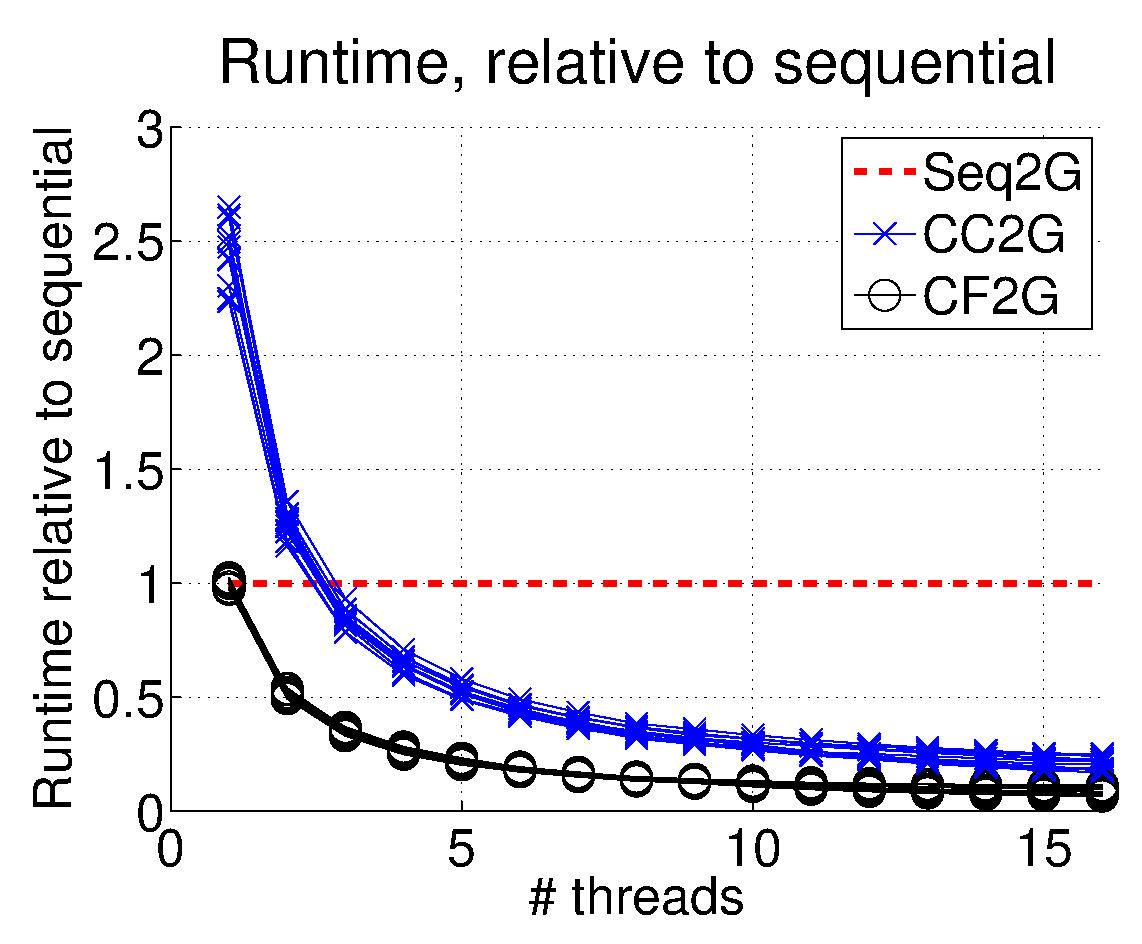
\includegraphics[width=130pt]{images/summary_relruntime.eps}
			\caption{}
			\label{fig:relruntime}
	  \end{subfigure} &
	  \begin{subfigure}[h]{0.30\textwidth}
	  	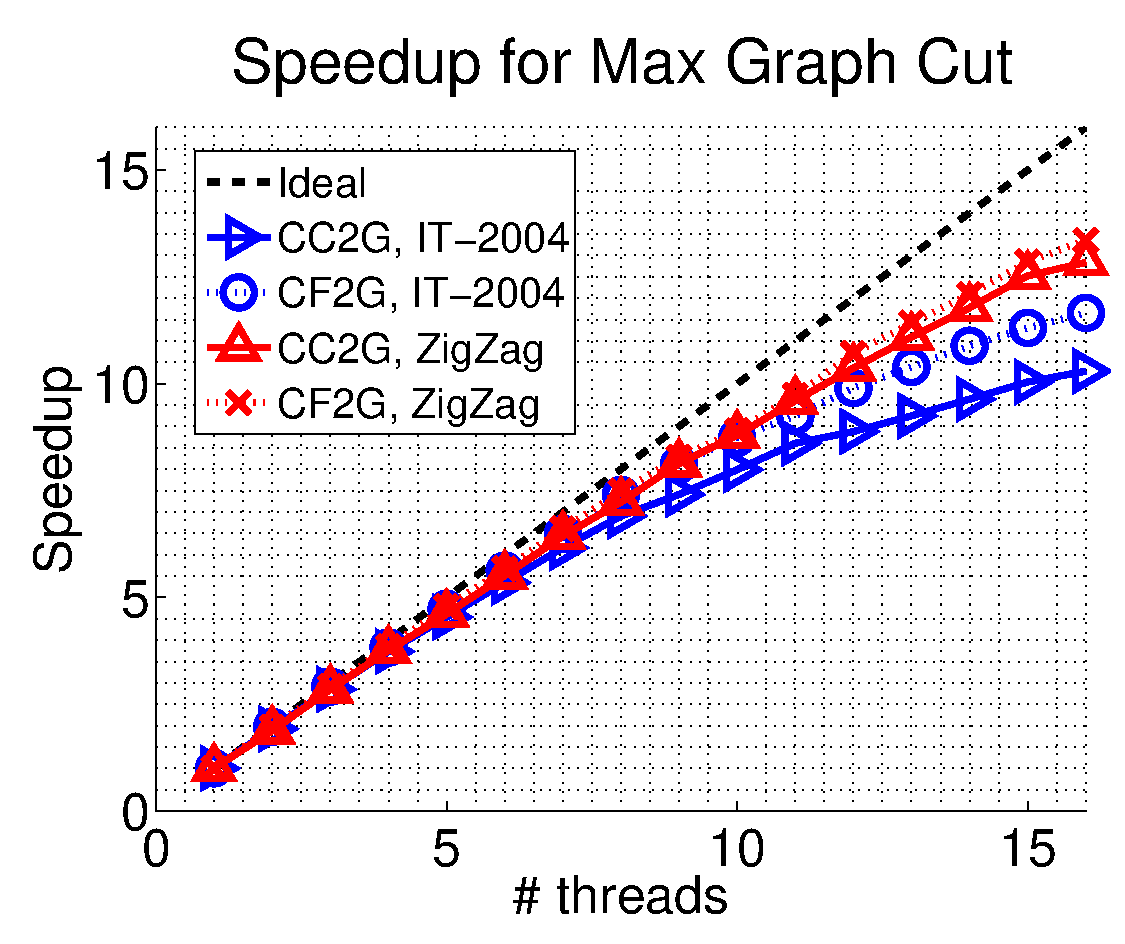
\includegraphics[width=130pt]{images/summary_speedup_maxgraphcut.eps}
			\caption{}
			\label{fig:speedup_maxgraphcut}
	  \end{subfigure} &
	  \begin{subfigure}[h]{0.30\textwidth}
	  	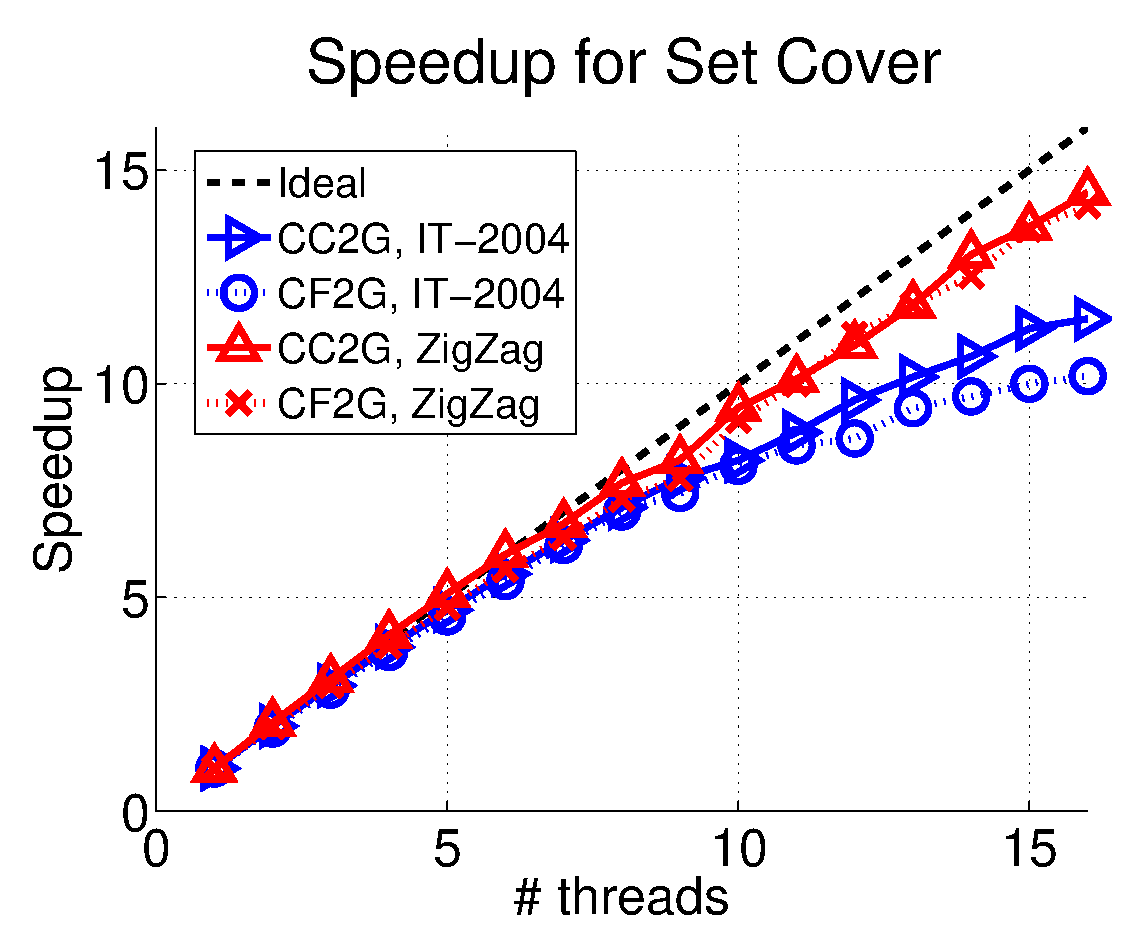
\includegraphics[width=130pt]{images/summary_speedup_setcover.eps}
			\caption{}
			\label{fig:speedup_setcover}
	  \end{subfigure} \\
	  \begin{subfigure}[h]{0.30\textwidth}
	  	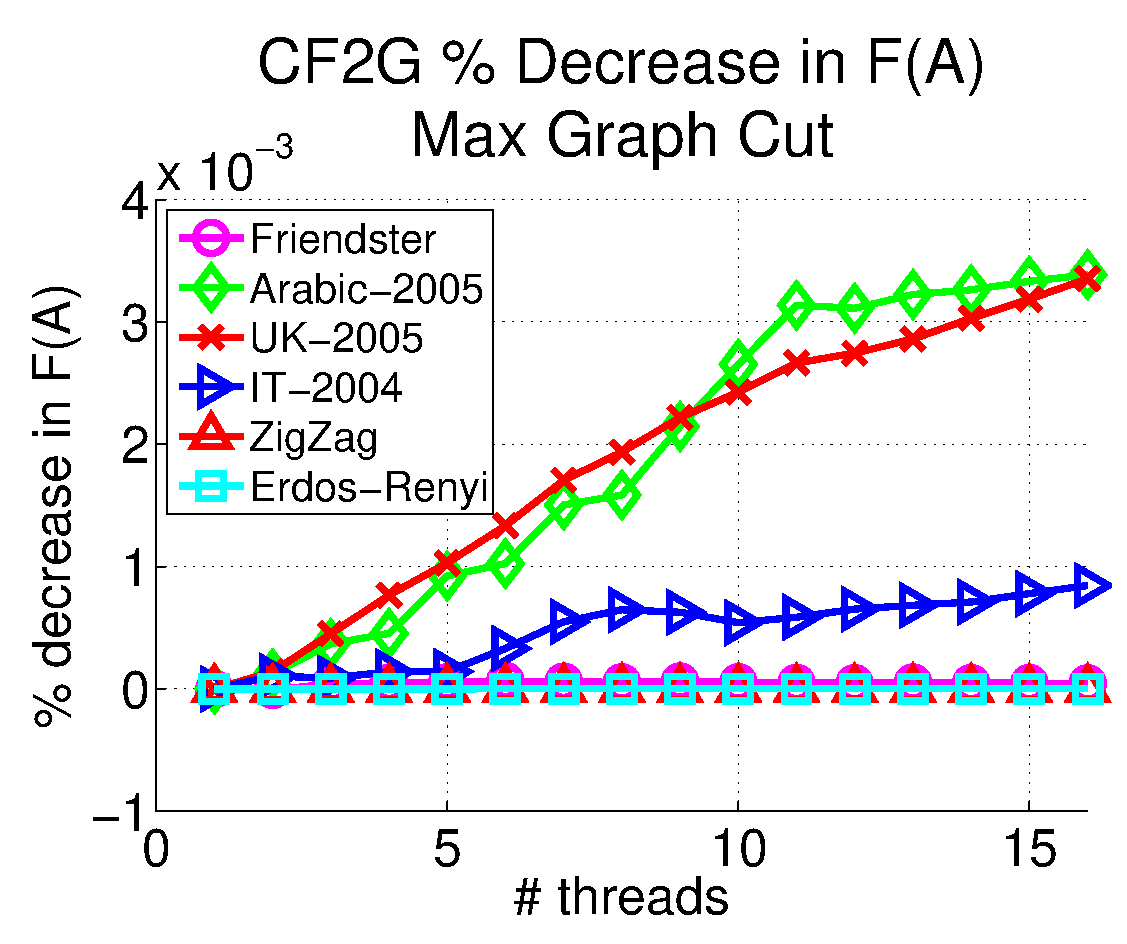
\includegraphics[width=130pt]{images/summary_diffFA_maxgraphcut.eps}
			\caption{}
			\label{fig:difffa_maxgraphcut}
	  \end{subfigure} &
	  \begin{subfigure}[h]{0.30\textwidth}
	  	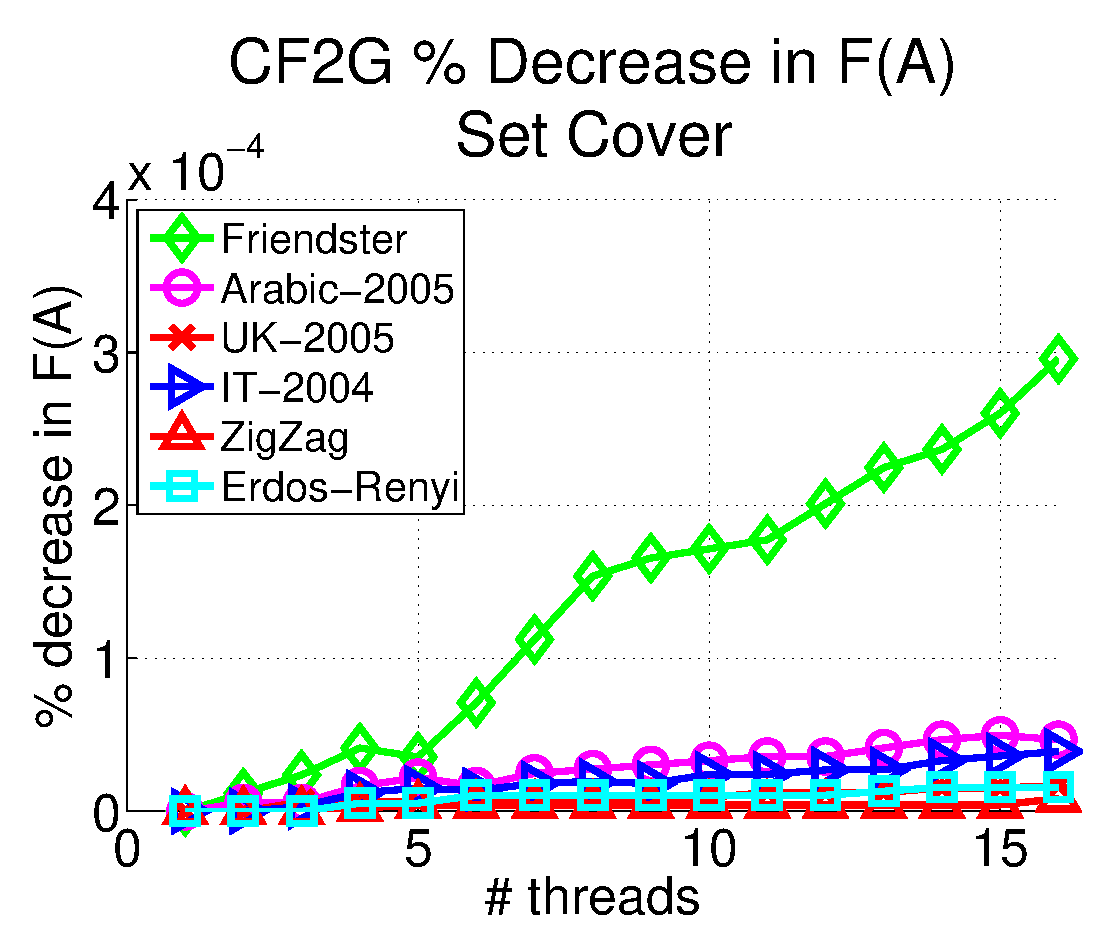
\includegraphics[width=130pt]{images/summary_diffFA_setcover.eps}
			\caption{}
			\label{fig:difffa_setcover}
	  \end{subfigure} &
	  \begin{subfigure}[h]{0.30\textwidth}
	  	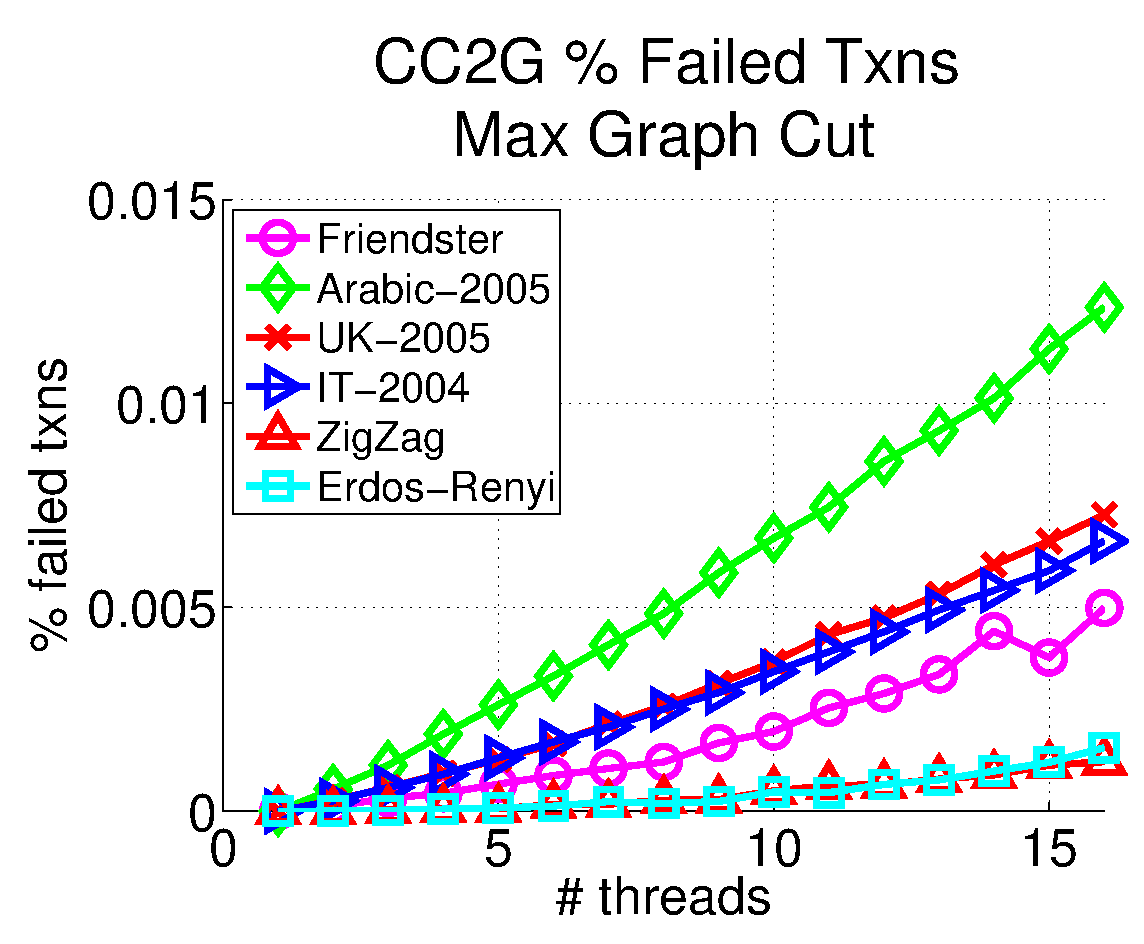
\includegraphics[width=130pt]{images/summary_validated_maxgraphcut.eps}
			\caption{}
			\label{fig:validated_maxgraphcut}
	  \end{subfigure} \\
  \end{tabular}
  \caption{\footnotesize Experimental results.
  Fig \ref{fig:relruntime} -- runtime of the parallel algorithms as a ratio to that of the sequential algorithm. Each curve shows the runtime of a parallel algorithm on a particular graph for a particular function $F$.
  Fig \ref{fig:speedup_maxgraphcut}, \ref{fig:speedup_setcover} -- speedup (ratio of runtime on one thread to that on $p$ threads).
  Fig \ref{fig:difffa_maxgraphcut}, \ref{fig:difffa_setcover} -- \% difference between objective values of the sequential and \hogwild{} algorithms, i.e. $[F(A_{\hogwild{}}) / F(A_{\seqalg}) - 1] \times 100\%$.
  Fig \ref{fig:validated_maxgraphcut} -- percentage of elements validated by the \occ{} algorithm on the max graph cut problem.
  }
\label{fig:results_quality}
\end{figure}


Due to space constraints, we only present part of our results in Figure \ref{fig:results_quality}, deferring full results to Appendix \ref{app:exptresults}.
\textbf{Runtime, Speedup:} Both parallel algorithms are faster than the sequential algorithm with three or more threads, and show good speedup properties as more threads are added ($\sim$ 10x or more for all graphs and both functions).
\textbf{Objective value:} The objective value of the \hogwild{} algorithm decreases with the number of threads, but differs from the sequential objective value by less than $0.01\%$.
\textbf{Validations:} The \occ{} algorithm validates more elements as threads are added, but less than 0.015\% are validated with 16 threads, which has negligible effect on the runtime / speedup.

\subsection{Adversarial ordering}

To highlight the philosophical differences between the two parallel algorithms, we conducted experiments on a ring Cayley graph on $\mathbb{Z}_{10^6}$ with generating set $\{\pm 1,\dots, \pm 1000\}$.
The algorithms are presented with an adversarial ordering, with permutation, so vertices close in the ordering are adjacent to one another, and tend to be processed concurrently.
This causes \hogwild{} to make more mistakes, and \occ{}to face more uncertainty.

As Figure \ref{fig:results_adversarial} shows, \occ{}sacrifices speed to ensure serial equivalence, eventually validating $>90\%$ of elements.
On the other hand, \hogwild{} focuses on speed, resulting in faster runtime, but delivering an objective value $F(A_{\hogwild{}})$ that is only $20\%$ of $F(A_{Seq2G})$.
For the set cover problem, we maintain statistics that are updated atomically by both algorithms.
The adversarial ordering forces more concurrent atomic updates, and hence, \hogwild{} does not achieve good speedup.
\footnote{We could have reduced coordination by computing $F$ directly, but doing so would result in longer runtimes.}

\begin{figure}[ht]
  \centering
  \begin{tabular}{cccc}
	  \begin{subfigure}[h]{0.30\textwidth}
	  	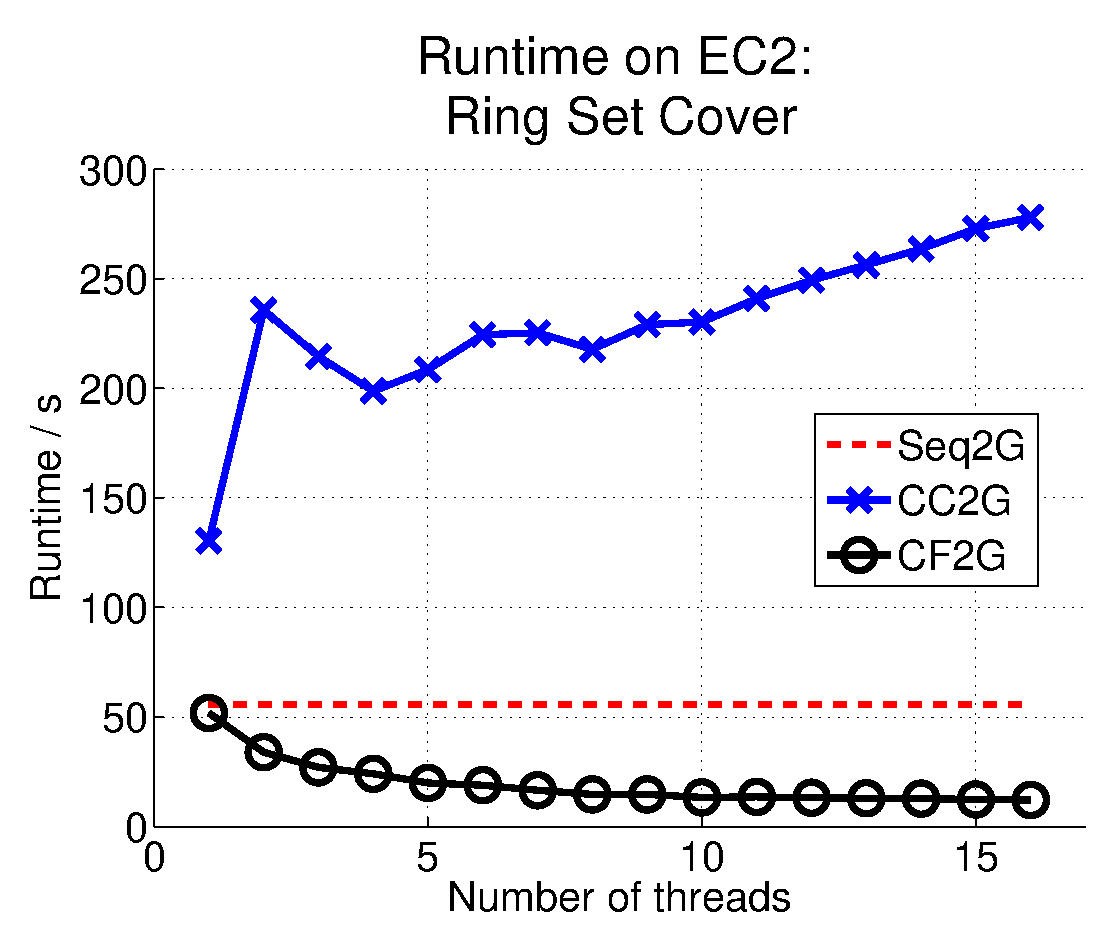
\includegraphics[width=130pt]{images/runtime_ring_setcover.eps}
			\caption{}
			\label{fig:runtime_ring_setcover}
	  \end{subfigure} &
	  \begin{subfigure}[h]{0.30\textwidth}
	  	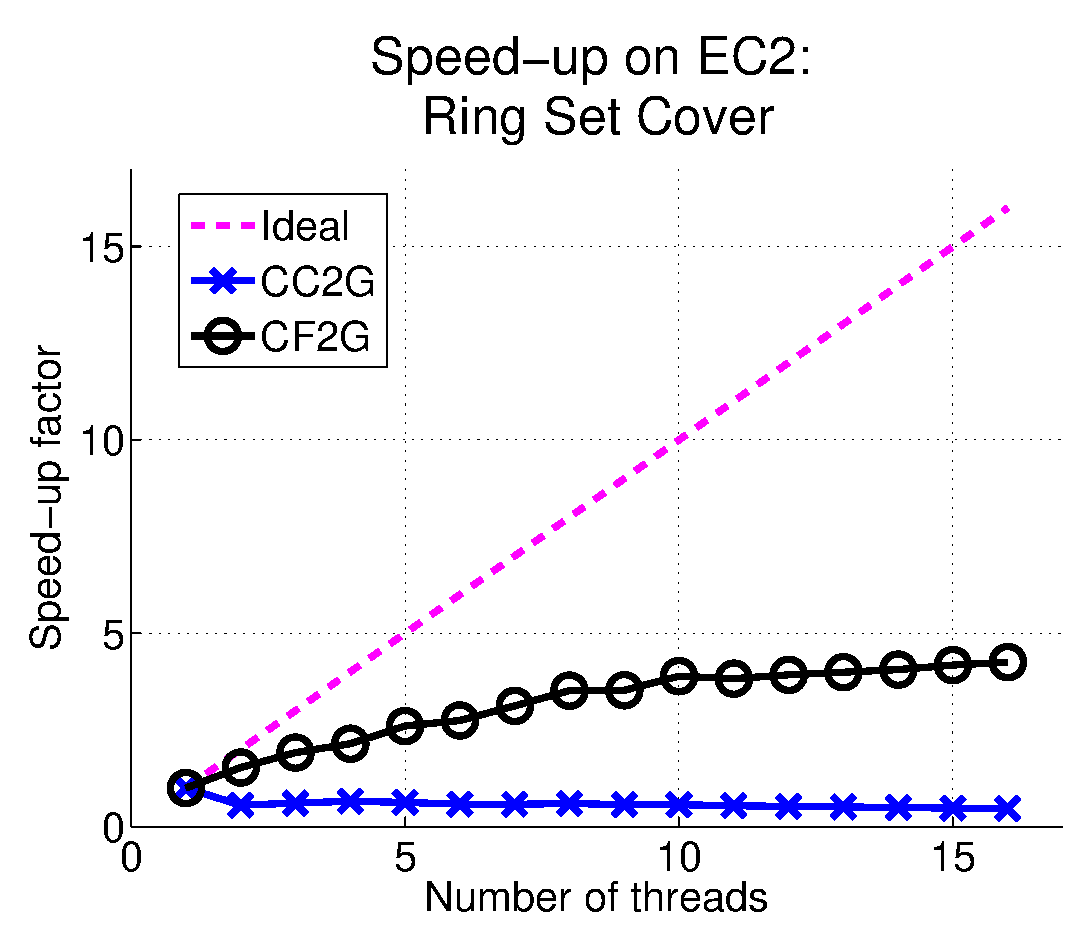
\includegraphics[width=130pt]{images/speedup_ring_setcover.eps}
			\caption{}
			\label{fig:speedup_ring_setcover}
	  \end{subfigure} &
	  \begin{subfigure}[h]{0.30\textwidth}
	  	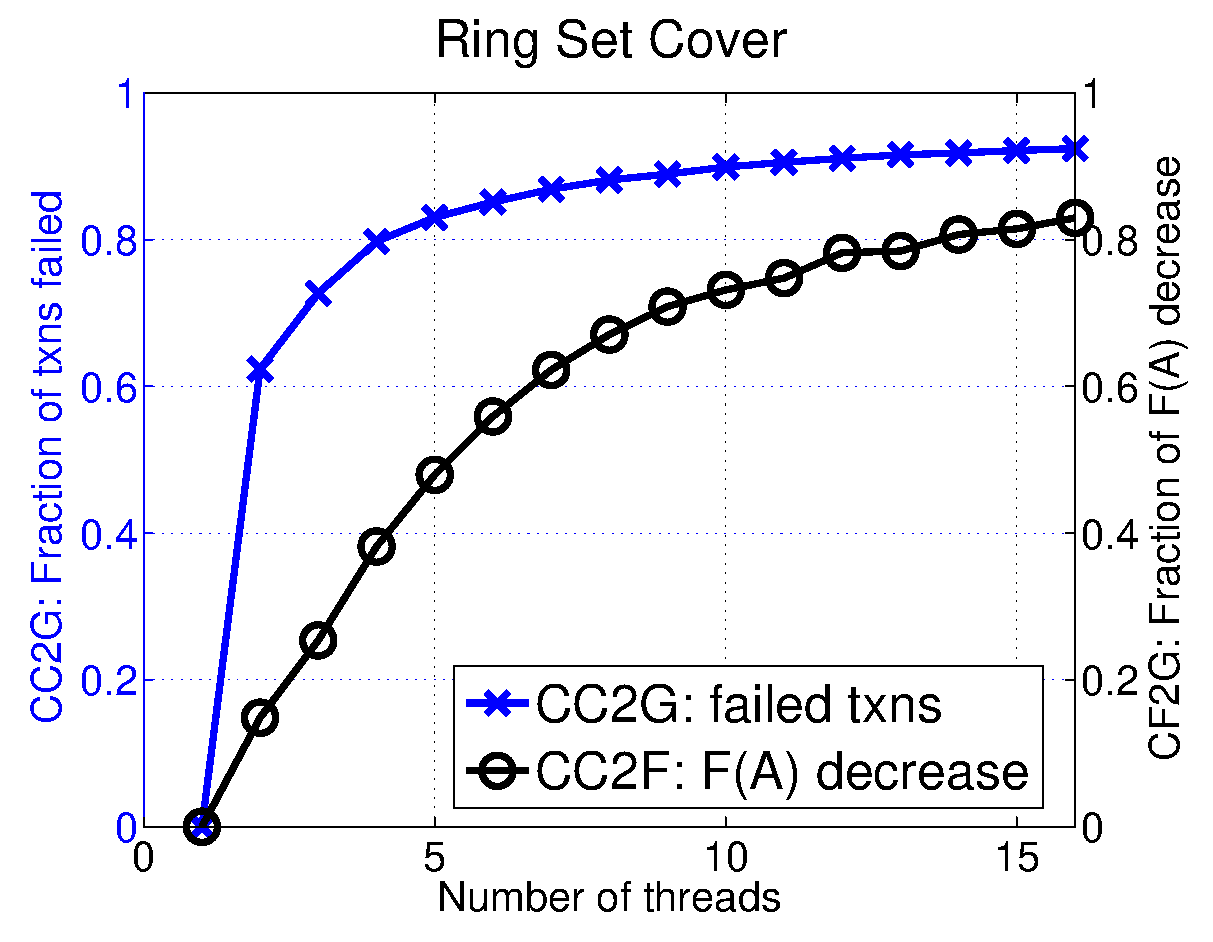
\includegraphics[width=130pt]{images/validateddiffFA_ring_setcover.eps}
			\caption{}
			\label{fig:validateddiffFA_ring_setcover}
	  \end{subfigure} \\
  \end{tabular}
  \caption{\footnotesize Experimental results for ring graph on set cover problem.}
\label{fig:results_adversarial}
\end{figure}

% \xinghao{These experiments were conducted by using an atomic integer to select elements to process. We could instead use a partitioning scheme, which has 2 advantages. Firstly, there is less coordination -- for \hogwild{}, we essentially have no coordination.
% Secondly, when faced with an adversarial ordering, the partitioning scheme allows big jumps / re-orderings, which reduces the number of validations and \textit{increases} the objective value of both parallel algorithms.}

We point out by using a partitioning scheme, it is possible to avoid the problems caused by the adversarial ordering, and to improve scalability.
Nevertheless, we present results that do use the partitioning scheme, so as to better highlight the differences between the two parallel algorithms.









\section{Related Work}
\textbf{Similar approach, different problem: } \occ{} DP-means \cite{pan2013}; \hogwild{} SGD \cite{Recht11}; \hogwild{} LDA \cite{Ahmed12} / parameter servers \cite{li2013, ho2013}

\textbf{Similar problem, different approach: } distributed greedy submodular maximization for monotone functions \cite{Mirzasoleiman2013}






\section{Discussions}

Conclusion: \xinghao{link back to intro, motivation}; we present two approaches to parallelizing unconstrained submodular maximization, which allows one to choose between speed and tight approximation guarantees.

Future work: constrained maximization, minimization; distributed setting, where communication costs and delays are higher, and function evaluations are challenging.


{\footnotesize
%\subsection*{Acknowledgments}
%This research is supported in part by NSF CISE Expeditions award CCF-1139158 and DARPA XData Award FA8750-12-2-0331, and  gifts from Amazon Web Services, Google, SAP,  Blue Goji, Cisco, Clearstory Data, Cloudera, Ericsson, Facebook, General Electric, Hortonworks, Intel, Microsoft, NetApp, Oracle, Samsung, Splunk, VMware and Yahoo!.
%This material is also based upon work supported in part by the Office of
%Naval Research under contract/grant number N00014-11-1-0688.
%X. Pan's work is also supported in part by a DSO National Laboratories Postgraduate Scholarship.

% In the unusual situation where you want a paper to appear in the
% references without citing it in the main text, use \nocite
%\nocite{langley00}

\bibliographystyle{unsrtnat}
\bibliography{references_arxiv}
}

\newpage
\appendix


\section{Parallel algorithms for separable sums}
\label{sec:sepsum}
\begin{figure}[h]
  \footnotesize
  \centering
  \begin{multicols}{2}
    \begin{minipage}{0.49\textwidth}
      \begin{algorithm}[H]
        \DontPrintSemicolon
        \caption{\hogwild{} for separable sums}
        \label{alg:hogwildsepsum}
        \lFor{$e\in V$}{$\hat{A}(e) = 0$}\;
        \lFor{$l = 1,\dots,L$}{$\hat\alpha_l = 0$, $\hat\beta_l = \sum_{e\in S_l}w_l(e)$}\;
        \ParForAll{$p \in \set{1, \ldots, P}$}{
          \While{$\exists$ element to process}{
            $e = $ next element to process\;
            $\Delta_+^{\max}(e) = -\lambda v(e) + \sum_{S_l\ni e} g(\hat\alpha_l + w_l(e)) - g(\hat\alpha_l)$\;
            $\Delta_-^{\max}(e) = +\lambda v(e) + \sum_{S_l\ni e} g(\hat\beta_l   - w_l(e)) - g(\hat\beta_l)$\;
            Draw $u_e\sim Unif(0,1)$\;
            \If {$u_e<\frac{[\Delta_{+}^{\max}(e)]_+}{[\Delta_{+}^{\min}(e)]_+ + [\Delta_{-}^{\max}(e)]_+}$}{
              $\hat{A}(e) \leftarrow 1$\;
              \lFor{$l: e \in S_l$}{
                $\hat\alpha_l \leftarrow \hat\alpha_l + w_l(e)$
              }
            }\lElse{
              \lFor{$l: e \in S_l$}{
                $\hat\beta_l \leftarrow \hat\beta_l - w_l(e)$
              }
            }
          }
        }
      \end{algorithm}
      \begin{algorithm}[H]
        \DontPrintSemicolon
        \caption{\occ{} validate for separable sums}
        \label{alg:occvalidate}
        \WaitUntil $\forall j < i$, processed$(j) = true$\;
        $\Delta_+^{\text{exact}}(e) = -\lambda v(e) + \sum_{S_l\ni e} g(\hat\alpha_l + w_l(e)) - g(\hat\alpha_l)$\;
        $\Delta_-^{\text{exact}}(e) = +\lambda v(e) + \sum_{S_l\ni e} g(\hat\beta_l   - w_l(e)) - g(\hat\beta_l)$\;
        \lIf {$u_e < \frac{[\Delta_+^{\text{exact}}(e)]_+}{[\Delta_+^{\text{exact}}(e)]_+ + [\Delta_-^{\text{exact}}(e)]_+}$}{
          result$(i) \leftarrow 1$\;
        }\lElse{
          result$(i) \leftarrow -1$\;
        }
      \end{algorithm}

    \end{minipage}

    \begin{minipage}{0.49\textwidth}
      \begin{algorithm}[H]
        \DontPrintSemicolon
        \caption{\occ{} for separable sums}
        \label{alg:occsepsum}
        \lFor{$e\in V$}{$\hat{A}(e) = \tilde{A}(e) = 0$, $\hat{B}(e) = \tilde{B}(e) = 1$}\;
        \For{$l = 1,\dots,L$}{
          $\hat\alpha_l = \tilde\alpha_l = 0$\;
          $\hat\beta_l = \tilde\beta_l = \sum_{e\in S_l}w_l(e)$\;
        }
        \lFor{$i = 1,\dots,|V|$}{result$(i) = 0$}\;
        \lFor{$i = 1,\dots,|V|$}{processed$(i) = false$}\;
        $\iota = 0$\;
        \ParForAll{$p \in \set{1, \ldots, P}$}{
          \While{$\exists$ element to process}{
            $e = $ next element to process\;
            $\tilde{A}(e) \leftarrow 1$\;
            $\tilde{B}(e) \leftarrow 0$\;
            \For{$l: e \in S_l$}{
              $\tilde\alpha_l \leftarrow \tilde\alpha_l + w_l(e)$\;
              $\tilde\beta_l  \leftarrow \tilde\beta_l  - w_l(e)$\;
            }
            $i = \iota$; $\iota \leftarrow \iota + 1$\;
            $\Delta_+^{\min}(e) = -\lambda v(e) + \sum_{S_l\ni e} g(\tilde\alpha_l) - g(\tilde\alpha_l - w_l(e))$\;
            $\Delta_+^{\max}(e) = -\lambda v(e) + \sum_{S_l\ni e} g(\hat\alpha_l + w_l(e)) - g(\hat\alpha_l)$\;
            $\Delta_-^{\min}(e) = +\lambda v(e) + \sum_{S_l\ni e} g(\tilde\beta_l) - g(\tilde\beta_l + w_l(e))$\;
            $\Delta_-^{\max}(e) = +\lambda v(e) + \sum_{S_l\ni e} g(\hat\beta_l   - w_l(e)) - g(\hat\beta_l)$\;
            Draw $u_e \sim Unif(0,1)$\;
            \If {$u_e < \frac{[\Delta_+^{\min}(e)]_+}{[\Delta_+^{\min}(e)]_+ + [\Delta_-^{\max}(e)]_+}$}{
              result$(i) \leftarrow 1$\;
            }\ElseIf {$u_e > \frac{[\Delta_+^{\max}(e)]_+}{[\Delta_+^{\max}(e)]_+ + [\Delta_-^{\min}(e)]_+}$}{
              result$(i) \leftarrow -1$\;
            }
            \WaitUntil $\forall j<i$, result$(j) \neq 0$\;
            \lIf {result$(i) = 0$}{validate($p$, $e$, $i$)}\;
            \If {result$(i) = 1$}{
              $\hat{A}(e)   \leftarrow 1$\;
              $\tilde{B}(e) \leftarrow 1$\;
              \For{$l: e \in S_l$}{
                $\hat\alpha_l   \leftarrow \hat\alpha_l   + w_l(e)$\;
                $\tilde\beta_l  \leftarrow \tilde\beta_l  + w_l(e)$\;
              }
            }\Else{
              $\tilde{A}(e) \leftarrow 0$\;
              $\hat{B}(e)   \leftarrow 0$\;
              \For{$l: e \in S_l$}{
                $\tilde\alpha_l \leftarrow \tilde\alpha_l - w_l(e)$\;
                $\hat\beta_l    \leftarrow \hat\beta_l    - w_l(e)$\;
              }
            }
            processed$(i) = true$\;
          }
        }
      \end{algorithm}
    \end{minipage}
  \end{multicols}
\end{figure}

For some functions $F$, we can maintain sketches / statistics to aid the computation of $\Delta_+^{\max}$, $\Delta_-^{\max}$, $\Delta_+^{\min}$, $\Delta_-^{\min}$.
In particular, we consider functions of the form
$F(X) = \sum_{l=1}^L g\left(\sum_{i\in X\cup S_l} w_l(i)\right) - \lambda\sum_{i\in X} v(i)$,
where $S_l \subseteq V$ are (possibly overlapping) groups of elements in the ground set, $g$ is a non-decreasing concave scalar function, and $w_l(i)$ and $v(i)$ are non-negative scalar weights.
It is easy to see that
$
F(X \cup e) - F(X) = \sum_{l: e\in S_l} \left[g\left(w_l(e) + \sum_{i\in X\cup S_l} w_l(i)\right) - g\left(\sum_{i\in X\cup S_l} w_l(i)\right)\right] - \lambda v(e)$.
Define
%  $\hat\alpha_l              = \sum_{j\in \hat{A}\cup S_l} w_l(j)$,
% $\hat\alpha_{l,e}          = \sum_{j\in \hat{A}_e\cup S_l} w_l(j)$,
% $\alpha_l^{\iota(e)-1} = \sum_{j\in A^{\iota(e)-1}\cup S_l} w_l(j)$.
%
%  $\hat\beta_l              = \sum_{j\in \hat{B}\cup S_l} w_l(j)$,
% $\hat\beta_{l,e}          = \sum_{j\in \hat{B}_e\cup S_l} w_l(j)$,
% $\beta_l^{\iota(e)-1} = \sum_{j\in B^{\iota(e)-1}\cup S_l} w_l(j)$.
%
\begin{align*}
  \hat\alpha_l              &= \sum_{j\in \hat{A}\cup S_l} w_l(j),
& \hat\alpha_{l,e}          &= \sum_{j\in \hat{A}_e\cup S_l} w_l(j),
& \alpha_l^{\iota(e)-1} &= \sum_{j\in A^{\iota(e)-1}\cup S_l} w_l(j).\\
  \hat\beta_l              &= \sum_{j\in \hat{B}\cup S_l} w_l(j),
& \hat\beta_{l,e}          &= \sum_{j\in \hat{B}_e\cup S_l} w_l(j),
& \beta_l^{\iota(e)-1} &= \sum_{j\in B^{\iota(e)-1}\cup S_l} w_l(j).
\end{align*}


\subsection{\hogwild{} for separable sums $F$}
Algorithm \ref{alg:hogwildsepsum} updates $\hat\alpha_l$ and $\hat\beta_l$, and computes $\Delta_+^{\max}(e)$ and $\Delta_-^{\max}(e)$ using $\hat\alpha_{l,e}$ and $\hat\beta_{l,e}$.
Following arguments analogous to that of Lemma \ref{lem:hog:set_bound}, we can show:

\begin{lem} For each $l$ and $e\in V$, $\hat\alpha_{l,e} \leq \alpha_l^{\iota(e)-1}$ and $\hat\beta_{l,e} \geq \beta_l^{\iota(e)-1}$.
\end{lem}

\begin{cor} Concavity of $g$ implies that $\Delta$'s computed by Algorithm \ref{alg:hogwildsepsum} satisfy
\begin{align*}
\Delta_+^{\max}(e)
&&\geq&& \sum_{S_l\ni e} \left[g(\alpha_l^{\iota(e)-1} + w_l(e)) - g(\alpha_l^{\iota(e)-1})\right] - \lambda v(e)
&&=&& \Delta_+(e),\\
\Delta_-^{\max}(e)
&&\geq&& \sum_{S_l\ni e} \left[g(\beta_l^{\iota(e)-1} - w_l(e)) - g(\beta_l^{\iota(e)-1})\right] + \lambda v(e)
&&=&& \Delta_-(e),
\end{align*}
\end{cor}

\subsection{\occ{} for separable sums $F$}
Analogous to the \hogwild{} algorithm, we maintain $\hat\alpha_l$, $\hat\beta_l$ and additionally $\tilde\alpha_l = \sum_{j\in \tilde{A}\cup S_l} w_l(j)$ and $\tilde\beta_l = \sum_{j \in \tilde{B}\cup S_l} w_l(j)$.
Following the arguments of Lemma \ref{lem:occ:set_bound} and Corollary \ref{cor:occ:delta_bound}, we can show the following.
\begin{lem} $\hat\alpha_{l,e} \leq \alpha^{\iota(e)-1} \leq \tilde\alpha_{l,e} - w_l(e)$ and $\hat\beta_{l,e} \geq \beta^{\iota(e)-1} \geq \tilde\beta_{l,e} + w_l(e)$
\end{lem}

\begin{cor} Concavity of $g$ implies that the $\Delta$'s computed by Algorithm \ref{alg:occsepsum} satisfy:
\begin{align*}
\Delta_+^{\max}(e)
&= - \lambda v(e) + \sum_{S_l \ni e} \left[g(\hat\alpha_{l,e} + w_l(e)) - g(\hat\alpha_{l,e})\right]\\
&\geq - \lambda v(e) + \sum_{S_l \ni e} \left[g(\hat\alpha_l^{\iota(e)-1} + w_l(e)) - g(\hat\alpha_l^{\iota(e)-1})\right]
&&= \Delta_+(e)\\
&\geq - \lambda v(e) + \sum_{S_l \ni e} \left[g(\tilde\alpha_{l,e}) - g(\tilde\alpha_{l,e} - w_l(e))\right]
&&= \Delta_+^{\min}(e),\\
\Delta_-^{\max}(e)
&= \lambda v(e) + \sum_{S_l \ni e} \left[g(\hat\beta_{l,e} - w_l(e)) - g(\hat\beta_{l,e})\right]\\
&\geq \lambda v(e) + \sum_{S_l \ni e} \left[g(\hat\beta_l^{\iota(e)-1} - w_l(e)) - g(\hat\beta_l^{\iota(e)-1})\right]
&&= \Delta_-(e)\\
&\geq \lambda v(e) + \sum_{S_l \ni e} \left[g(\tilde\beta_l^{\iota(e)-1}) - g(\tilde\beta_l^{\iota(e)-1} + w_l(e))\right]
&&= \Delta_-^{\min}(e).
\end{align*}
\end{cor}


\newpage\section{Proof of bound for \hogwild{}}
\label{app:proofhogwild}


We follow the proof outline of \cite{buchbinder2012}.

Consider an ordering $\iota$ inducted by running \hogwild{}.
For convenience, we will use $i$ to flexibly denote the element $e$ and its ordering $\iota(e)$.

Let $OPT$ be an optimal solution to the problem.
Define $O^i := (OPT \cup A^i) \cap B^i$.
Note that $O^i$ coincides with $A^i$ and $B^i$ on elements $1,\dots,i$, and $O^i$ coincides with $OPT$ on elements $i+1,\dots, n$.
Hence,
\begin{align*}
O^i \backslash i+1 &\supseteq A^i \text{\stef{Is this $(i+1)$ or adding one?}}\\
O^i \cup i+1 &\subseteq B^i.
\end{align*}

\begin{lem}\label{lem:positivesum} For every $1 \leq i \leq n$, $\Delta_+(i) + \Delta_-(i) \geq 0$.
\end{lem}
\begin{proof} This is just Lemma II.1 of \cite{buchbinder2012}.
\end{proof}

\begin{lem}\label{lem:singleelement}
Let $\rho_i = \max\{\Delta_+^{\max}(e) - \Delta_+(e), \Delta_-^{\max}(e) - \Delta_-(e)\}$.
For every $1 \leq i \leq n$,
\[E[F(O^{i-1})-F(O^i)] \leq \frac{1}{2} E[F(A^i) - F(A^{i-1}) + F(B^i) - F(B^{i-1}) + \rho_i].\]
\end{lem}
\begin{proof}
We follow the proof outline of \cite{buchbinder2012}.
First, note that it suffices to prove the inequality conditioned on knowing $A^{i-1}$, $\hat{A}_i$ and $\hat{B}_i$, then applying the law of total expectation.
Under this conditioning, we also know $B^{i-1}$, $O^{i-1}$, $\Delta_+(i)$, $\Delta_+^{\max}(i)$, $\Delta_-(i)$, and $\Delta_-^{\max}(i)$.



We consider the following 6 cases.


\begin{description}

\item\textbf{Case 1:} $0 < \Delta_+(i) \leq \Delta_+^{\max}(i)$, $0 \leq \Delta_-^{\max}(i)$.
Since both $\Delta_+^{\max}(i)>0$ and $\Delta_-^{\max}(i)>0$, the probability of including $i$ is just $\Delta_+^{\max}(i) / (\Delta_+^{\max}(i) + \Delta_-^{\max}(i))$, and the probability of excluding $i$ is $\Delta_-^{\max}(i) / (\Delta_+^{\max}(i) + \Delta_-^{\max}(i))$.
\begin{align*}
E[F(A^i) - F(A^{i-1}) | A^{i-1}, \hat{A}_i, \hat{B}_i]
&= \frac{\Delta_+^{\max}(i)}{\Delta_+^{\max}(i) + \Delta_-^{\max}(i)} (F(A^{i-1}\cup i) - F(A^{i-1}))\\
&= \frac{\Delta_+^{\max}(i)}{\Delta_+^{\max}(i) + \Delta_-^{\max}(i)} \Delta_+(i)\\
&\geq \frac{\Delta_+^{\max}(i)}{\Delta_+^{\max}(i) + \Delta_-^{\max}(i)} (\Delta_+^{\max}(i) - \rho_i)\\
E[F(B^i) - F(B^{i-1}) | A^{i-1}, \hat{A}_i, \hat{B}_i]
&= \frac{\Delta_-^{\max}(i)}{\Delta_+^{\max}(i) + \Delta_-^{\max}(i)} (F(B^{i-1}\backslash i) - F(B^{i-1}))\\
&= \frac{\Delta_-^{\max}(i)}{\Delta_+^{\max}(i) + \Delta_-^{\max}(i)} \Delta_-(i)\\
&\geq \frac{\Delta_-^{\max}(i)}{\Delta_+^{\max}(i) + \Delta_-^{\max}(i)} (\Delta_-^{\max}(i) - \rho_i)
\end{align*}
\begin{align*}
&E[F(O^{i-1}) - F(O^i) | A^{i-1}, \hat{A}_i, \hat{B}_i]\\
=&   \frac{\Delta_+^{\max}(i)}{\Delta_+^{\max}(i) + \Delta_-^{\max}(i)} (F(O^{i-1}) - F(O^{i-1} \cup i)) \\
 & + \frac{\Delta_-^{\max}(i)}{\Delta_+^{\max}(i) + \Delta_-^{\max}(i)} (F(O^{i-1}) - F(O^{i-1} \backslash i)) \\
=&\begin{cases}
    \frac{\Delta_+^{\max}(i)}{\Delta_+^{\max}(i) + \Delta_-^{\max}(i)} (F(O^{i-1}) - F(O^{i-1} \cup i))       & \text{if $i\not\in OPT$}\\
    \frac{\Delta_-^{\max}(i)}{\Delta_+^{\max}(i) + \Delta_-^{\max}(i)} (F(O^{i-1}) - F(O^{i-1} \backslash i)) & \text{if $i    \in OPT$}\\
\end{cases}\\
\leq&\begin{cases}
    \frac{\Delta_+^{\max}(i)}{\Delta_+^{\max}(i) + \Delta_-^{\max}(i)} (F(B^{i-1}\backslash i) - F(B^{i-1})) & \text{if $i\not\in OPT$}\\
    \frac{\Delta_-^{\max}(i)}{\Delta_+^{\max}(i) + \Delta_-^{\max}(i)} (F(A^{i-1}\cup i) - F(A^{i-1}))       & \text{if $i    \in OPT$}\\
\end{cases}\\
=&\begin{cases}
    \frac{\Delta_+^{\max}(i)}{\Delta_+^{\max}(i) + \Delta_-^{\max}(i)} \Delta_-(i) & \text{if $i\not\in OPT$}\\
    \frac{\Delta_-^{\max}(i)}{\Delta_+^{\max}(i) + \Delta_-^{\max}(i)} \Delta_+(i) & \text{if $i    \in OPT$}\\
\end{cases}\\
\leq&\begin{cases}
    \frac{\Delta_+^{\max}(i)}{\Delta_+^{\max}(i) + \Delta_-^{\max}(i)} \Delta_-^{\max}(i) & \text{if $i\not\in OPT$}\\
    \frac{\Delta_-^{\max}(i)}{\Delta_+^{\max}(i) + \Delta_-^{\max}(i)} \Delta_+^{\max}(i) & \text{if $i    \in OPT$}\\
\end{cases}\\
=& \frac{\Delta_+^{\max}(i)\Delta_-^{\max}(i)}{\Delta_+^{\max}(i) + \Delta_-^{\max}(i)}
\end{align*}
where the first inequality is due to submodularity: $O^{i-1}\backslash i \supseteq A^{i-1}$ and $O^{i-1}\cup i \subseteq B^{i-1}$.

Putting the above inequalities together:
\begin{align*}
&E\left[F(O^{i-1}) - F(O^i) - \frac{1}{2} \bigg(F(A^i) - F(A^{i-1}) + F(B^i) - F(B^{i-1}) + \rho_i\bigg) \bigg| A^{i-1}, \hat{A}_i, \hat{B}_i\right]\\
&\leq \frac{1/2}{\Delta_+^{\max}(i) + \Delta_-^{\max}(i)}\bigg[
2\Delta_+^{\max}(i)\Delta_-^{\max}(i)
- \Delta_-^{\max}(i)(\Delta_-^{\max}(i) - \rho_i)\\
&\quad\quad\quad\quad\quad\quad\quad\quad\quad\quad- \Delta_+^{\max}(i)(\Delta_+^{\max}(i) - \rho_i)
\bigg]- \frac{1}{2}\rho_i\\
&= \frac{1/2}{\Delta_+^{\max}(i) + \Delta_-^{\max}(i)}\bigg[-(\Delta_+^{\max}(i) - \Delta_-^{\max}(i))^2 + \rho_i(\Delta_+^{\max}(i) + \Delta_-^{\max}(i))\bigg] - \frac{1}{2}\rho_i\\
&\leq \frac{\frac{1}{2}\rho_i(\Delta_+^{\max}(i) + \Delta_-^{\max}(i))}{\Delta_+^{\max}(i) + \Delta_-^{\max}(i)} - \frac{1}{2}\rho_i\\
&= 0.
\end{align*}

\item\textbf{Case 2:} $0 < \Delta_+(i) \leq \Delta_+^{\max}(i)$, $\Delta_-^{\max}(i) < 0$.
In this case, the algorithm always choses to include $i$, so $A^i = A^{i-1} \cup i$, $B^i = B^{i-1}$ and $O^i = O^{i-1} \cup i$:
\begin{align*}
E[F(A^i) - F(A^{i-1}) | A^{i-1}, \hat{A}_i, \hat{B}_i] &= F(A^{i-1} \cup i) - F(A^{i-1}) = \Delta_+(i) > 0\\
E[F(B^i) - F(B^{i-1}) | A^{i-1}, \hat{A}_i, \hat{B}_i] &= F(B^{i-1}) - F(B^{i-1}) = 0\\
E[F(O^{i-1}) - F(O^i) | A^{i-1}, \hat{A}_i, \hat{B}_i] &= F(O^{i-1}) - F(O^{i-1} \cup i) \\
&\leq \begin{cases}0 & \text{if $i\in OPT$} \\ F(B^{i-1} \backslash i) - F(B^{i-1}) & \text{if $i\not\in OPT$}\end{cases}\\
&= \begin{cases}0 & \text{if $i\in OPT$} \\ \Delta_-(i) & \text{if $i\not\in OPT$}\end{cases}\\
&\leq 0\\
&< \frac{1}{2} E[F(A^i) - F(A^{i-1}) + F(B^i) - F(B^{i-1}) + \rho_i | A^{i-1}, \hat{A}_i, \hat{B}_i]
\end{align*}
where the first inequality is due to submodularity: $O^{i-1}\cup i \subseteq B^{i-1}$.


\item\textbf{Case 3:} $\Delta_+(i) \leq 0 < \Delta_+^{\max}(i)$, $0 < \Delta_-(i) < \Delta_-^{\max}(i)$.
Analogous to Case 1.



\item\textbf{Case 4:} $\Delta_+(i) \leq 0 < \Delta_+^{\max}(i)$, $\Delta_-(i) \leq 0$.
This is not possible, by Lemma \ref{lem:positivesum}.

\item\textbf{Case 5:} $\Delta_+(i) \leq \Delta_+^{\max}(i) \leq 0$, $0 < \Delta_-(i) \leq \Delta_-^{\max}(i)$.
Analogous to Case 2.

\item\textbf{Case 6:} $\Delta_+(i) \leq \Delta_+^{\max}(i) \leq 0$, $\Delta_-(i) \leq 0$.
This is not possible, by Lemma \ref{lem:positivesum}.


\end{description}
\end{proof}







\begin{comment}

(\xinghao{Note} If we weaken the assumption of $\Delta_+(i) \leq \Delta_+^{\max}(i)$ to $\Delta_+(i) \leq \Delta_+^{\max}(i) + \epsilon_i$, then in Case 6 above, we can instead bound
\begin{align*}
E[F(O^{i-1})-F(O^i)|A^{i-1}, j]
&\leq \frac{\Delta_+^{\max}(i) \Delta_-^{\max}(i) + \epsilon\max(\Delta_+^{\max}(i), \Delta_-^{\max})}{\Delta_+^{\max}(i) + \Delta_-^{\max}(i)}\\
&\leq \frac{\Delta_+^{\max}(i) \Delta_-^{\max}(i) + \epsilon(\Delta_+^{\max}(i) + \Delta_-^{\max})}{\Delta_+^{\max}(i) + \Delta_-^{\max}(i)}.
\end{align*}
The bound of Lemma \ref{lem:singleelement} becomes
\[E[F(O^{i-1})-F(O^i)] \leq \frac{1}{2} E[F(A^i) - F(A^{i-1}) + F(B^i) - F(B^{i-1}) + \rho_i + 2\epsilon_i],\]
and the bound of Theorem \ref{thm:randomapprox} becomes $E[F(A)] \geq \frac{1}{2} F^* - \frac{1}{4}\sum_iE[\rho_i + 2\epsilon_i]$.
)

\end{comment}







We will now prove the main theorem.

\thmrandomapprox*

\begin{proof}
Summing up the statement of Lemma \ref{lem:singleelement} for all $i$ gives us a telescoping sum, which reduces to:
\begin{align*}
E[F(O^0)-F(O^n)]
&\leq \frac{1}{2} E[F(A^n) - F(A^0) + F(B^n) - F(B^0)] + \frac{1}{2}\sum_{i=1}^nE[\rho_i]\\
&\leq \frac{1}{2} E[F(A^n) + F(B^n)] + \frac{1}{2}\sum_{i=1}^nE[\rho_i].
\end{align*}
Note that $O^0 = OPT$ and $O^n = A^n = B^n$, so $E[F(A^n)] \geq \frac{1}{2} F^* - \frac{1}{4}\sum_iE[\rho_i]$.
\end{proof}









\subsection{Example: max graph cut}
Let $C_i = (A^{i-1}\backslash \hat{A}_i) \cup (\hat{B}_i\backslash B^{i-1})$ be the set of elements concurrently processed with $i$ but ordered after $i$, and $D_i = B^i\backslash A^i$ be the set of elements ordered after $i$.
Denote $\bar{A}_j = V\backslash \hat{A}_i\backslash C_i\backslash D_i = \{1,\dots,j\}\backslash \hat{A}_i$ be the elements up to $j$ that are not included in $A$ \stef{$\hat{A}^i$?}. \stef{Parentheses to help parse multiple setminuses}
Let $w_i(S) = \sum_{j\in S, (i,j)\in E} w(i,j)$.
For the max graph cut function, it is easy to see that \stef{what is the index $j$? any arbitrary index?}
\begin{align*}
\Delta_+        &\geq - w_i(\hat{A}_i) -w_i(C_i) + w_i(D_i) + w_i(\bar{A}_j)\\
\Delta_+^{\max} &=    - w_i(\hat{A}_i) + w_i(C_i) + w_i(D_i) + w_i(\bar{A}_j)\\
\Delta_-        &\geq + w_i(\hat{A}_i) - w_i(C_i) + w_i(D_i) - w_i(\bar{A}_j)\\
\Delta_-^{\max} &= + w_i(\hat{A}_i) + w_i(C_i) + w_i(D_i) - w_i(\bar{A}_j)
\end{align*}
\stef{If there is time, an illustration would maybe make things clear.}

Thus, we can see that $\rho_i \leq 2w_i(C_i)$.

Suppose we have bounded delay $\tau$, so $|C_i| \leq \tau$.
Then $w_i(C_i)$ has a hypergeometric distribution with mean $\frac{\text{deg}(i)}{N}\tau$, and $E[\rho_i] \leq 2\tau\frac{\text{deg}(i)}{N}$.
The approximation of the hogwild algorithm is then $E[F(A^n)] \geq \frac{1}{2} F^* - \tau\frac{\#\text{edges}}{2N}$.
In sparse graphs, the hogwild algorithm is off by a small additional term, which albeit grows linearly in $\tau$.
In a complete graph, $F^* = \frac{1}{2}\#\text{edges}$, so $E[F(A^n)] \geq F^*\left(\frac{1}{2} - \frac{\tau}{N}\right)$, which makes it possible to scale $\tau$ linearly with $N$ while retaining the same approximation factor.



\subsection{Example: set cover}
% \xinghao{For now, consider a toy problem, with (1) disjoint sets, (2) bounded delay, (3) $\lambda \leq 1$.}

Consider the simple set cover function, for $\lambda < L/N$:
\[ F(A) = \sum_{l=1}^L \min(1,|A\cap S_l|) - \lambda|A| = |\{l: A\cap S_l \neq\emptyset\}| - \lambda|A|.\]

We assume that there is some bounded delay $\tau$.

Suppose also that the sets $S_l$ form a partition, so each element $e$ belongs to exactly one set.
Let $n_l = |S_l|$ denote the size of $S_l$.
Given any ordering $\pi$, let $e_l^t$ be the $t$th element of $S_l$ in the ordering, i.e. $|\{e': \pi(e') \leq \pi(e_l^t) \wedge e'\in S_l\}| = t$.

For any $e \in S_l$, we get 
\begin{align*}
\Delta_+       (e) &= -\lambda + 1\{A^{\iota(e)-1}\cap S_l = \emptyset\}\\
\Delta_+^{\max}(e) &= -\lambda + 1\{\hat{A}_e\cap S_l = \emptyset\}\\
\Delta_-       (e) &= +\lambda - 1\{B^{\iota(e)-1}\backslash e\cap S_l = \emptyset\}\\
\Delta_-^{\max}(e) &= +\lambda - 1\{\hat{B}_e\backslash e\cap S_l = \emptyset\}
\end{align*}

Let $\eta$ be the position of the first element of $S_l$ to be accepted, i.e. $\eta = \min\{t : e_l^t \in A \cap S_l\}$.
(For convenience, we set $\eta = n_l$ if $A \cap S_l = \emptyset$.)
We first show that $\eta$ is independent of $\pi$: for $\eta < n_l$,
\begin{align*}
P(\eta|\pi)
&= \frac{\Delta_+^{\max}(e_l^\eta)}{\Delta_+^{\max}(e_l^\eta) + \Delta_-^{\max}(e_l^\eta)} \prod_{t=1}^{\eta-1} \frac{\Delta_-^{\max}(e_l^t)}{\Delta_+^{\max}(e_l^t) + \Delta_-^{\max}(e_l^t)}\\
&= \frac{1-\lambda}{1-\lambda+\lambda} \prod_{t=1}^{\eta-1} \frac{\lambda}{1-\lambda+\lambda}\\
&= (1-\lambda)\lambda^{\eta-1},
\end{align*}
and $P(\eta=n_l | \pi) = \lambda^{\eta-1}$.
% \xinghao{This independence depends on the assumption of disjoint sets, which in turn allows us to decouple the randomness of the algorithm from the randomness of ordering in the below proof.}

Note that, $\Delta_-^{\max}(e)-\Delta_-(e) = 1$ iff $e=e_l^{n_l}$ is the last element of $S_l$ in the ordering, there are no elements accepted up to $\hat{B}_{e_l^{n_l}}\backslash e_l^{n_l}$, and there is some element $e'$ in $\hat{B}_{e_l^{n_l}}\backslash {e_l^{n_l}}$ that is rejected and not in $B^{\iota(e_l^{n_l})-1}$.
Denote by $m_l \leq \min(\tau,n_l-1)$ the number of elements before $e_l^{n_l}$ that are inconsistent between $\hat{B}_{e_l^{n_l}}$ and $B^{\iota(e_l^{n_l})-1}$.
Then $\mathbb{E}[\Delta_-^{\max}(e_l^{n_l}) - \Delta_-(e_l^{n_l})] = P(\Delta_-^{\max}(e_l^{n_l}) \neq \Delta_-(e_l^{n_l}))$ is
\begin{align*}
\lambda^{n_l-1-m_l}(1-\lambda^{m_l})
&&=&& \lambda^{n_l-1}(\lambda^{-m_l}-1)
&&\leq&& \lambda^{n_l-1}(\lambda^{-\min(\tau,n_l-1)}-1)
&&\leq&& 1 - \lambda^\tau.
\end{align*}
If $\lambda=1$, $\Delta_+^{\max}(e) \leq 0$, so no elements before $e_l^{n_l}$ will be accepted, and $\Delta_-^{\max}(e_l^{n_l}) = \Delta_-(e_l^{n_l})$.

On the other hand, $\Delta_+^{\max}(e)-\Delta_+(e) = 1$ iff $(A^{\iota(e)-1}\backslash\hat{A}_e)\cap S_l \neq\emptyset$, that is, if an element has been accepted in $A$ but not yet observed in $\hat{A}_e$.
Since we assume a bounded delay, only the first $\tau$ elements after the first acceptance of an $e\in S_l$ may be affected.
\begin{align*}
&\mathbb{E}\left[\sum_{e\in S_l}\Delta_+^{\max}(e) - \Delta_+(e)\right]\\
&= \mathbb{E}[\#\{e: e \in S_l \wedge e_l^\eta \in A^{\iota(e)-1} \wedge e_l^\eta \not\in \hat{A}_e\}]\\
&= \mathbb{E}[\mathbb{E}[\#\{e: e \in S_l \wedge e_l^\eta \in A^{\iota(e)-1} \wedge e_l^\eta \not\in \hat{A}_e\} ~|~ \eta = t, \pi(e_l^t)=k]]\\
&= \sum_{t=1}^{n_l}\sum_{k=t}^{N-n+t} P(\eta=t, \pi(e_l^t)=k) \mathbb{E}[\#\{e: e \in S_l \wedge e_l^\eta \in A^{\iota(e)-1} \wedge e_l^\eta \not\in \hat{A}_e\} ~|~ \eta = t, \pi(e_l^t)=k]\\
&= \sum_{t=1}^{n_l} P(\eta=t) \sum_{k=t}^{N-n+t} P(\pi(e_l^t)=k) \mathbb{E}[\#\{e: e \in S_l \wedge e_l^\eta \in A^{\iota(e)-1} \wedge e_l^\eta \not\in \hat{A}_e\} ~|~ \eta = t, \pi(e_l^t)=k].
\end{align*}

Under the assumption that every ordering $\pi$ is equally likely, and a bounded delay $\tau$,
conditioned on $\eta = t, \pi(e_l^t)=k$, the random variable $\#\{e: e \in S_l \wedge e_l^\eta \in A^{\iota(e)-1} \wedge e_l^\eta \not\in \hat{A}_e\}$ has hypergeometric distribution with mean $\frac{n_l-t}{N-k}\tau$.
Also, $P(\pi(e_l^t) = k) = \frac{n_l}{N}{n-1 \choose t-1}{N-n \choose k-t} / {N-1 \choose k-1}$, so the above expression becomes
\begin{align*}
&\mathbb{E}\left[\sum_{e\in S_l}\Delta_+^{\max}(e) - \Delta_+(e)\right]\\
&= \sum_{t=1}^{n_l} P(\eta=t) \sum_{k=t}^{N-n+t} \frac{n_l}{N} \frac{{n-1 \choose t-1}{N-n \choose k-t}}{{N-1 \choose k-1}} \frac{n-t}{N-k} \tau\\
&= \frac{n_l}{N} \tau \sum_{t=1}^{n_l} P(\eta=t) \sum_{k=t}^{N-n+t} \frac{{k-1 \choose t-1}{N-k \choose n-t}}{{N-1 \choose n-1}} \frac{n-t}{N-k} & \text{(symmetry of hypergeometric)} \\
&= \frac{n_l}{N} \tau \sum_{t=1}^{n_l} \frac{P(\eta=t)}{{N-1 \choose n-1}} \sum_{k=t}^{N-n+t} {k-1 \choose t-1}{N-k-1 \choose n-t-1} \\
&= \frac{n_l}{N} \tau \sum_{t=1}^{n_l} \frac{P(\eta=t)}{{N-1 \choose n-1}} {N-1 \choose n-1} & \text{(Lemma \ref{lem:sumbinomial}, $a=N-2$, $b=n_l-2$, $j=1$)} \\
&= \frac{n_l}{N} \tau \sum_{t=1}^{n_l} P(\eta=t) \\
&= \frac{n_l}{N} \tau.
\end{align*}

Since $\Delta_+^{\max}(e) \geq \Delta_+(e)$ and $\Delta_-^{\max}(e) \geq \Delta_-^{\max}(e)$, we have that $\rho_e \leq \Delta_+^{\max}(e) - \Delta_+(e) + \Delta_-^{\max}(e) - \Delta_-(e)$, so
\begin{align*}
\mathbb{E}\left[\sum_e \rho_e\right]
&= \mathbb{E}\left[\sum_e \Delta_+^{\max}(e) - \Delta_+(e) + \Delta_-^{\max}(e) - \Delta_-(e) \right]\\
&= \sum_l \mathbb{E}\left[\sum_{e\in S_l} \Delta_+^{\max}(e) - \Delta_+(e)\right] + \mathbb{E}\left[\sum_{e\in S_l} \Delta_-^{\max}(e) - \Delta_-(e) \right]\\
&\leq \tau\frac{\sum_l n_l}{N} + L(1-\lambda^\tau)\\
&= \tau + L(1-\lambda^\tau).
\end{align*}
Note that $\mathbb{E}\left[\sum_e \rho_e\right]$ does not depend on $N$ and is linear in $\tau$.
Also, if $\tau=0$ in the sequential case, we get $\mathbb{E}\left[\sum_e \rho_e\right] \leq 0$.



\newpage\section{Upper bound on expected number of elements sent for validation}
\label{app:proofocc}
Let $N$ be the number of elements, i.e. the cardinality of the ground set.
Let $P$ be the number of processors.

We assume that the total ordering assigns elements to processors in a round robin fashion.
Thus, we assume $C^{ji}=\{i-p+1,\dots,i-1\}$ has $p-1$ elements.

We call element $i$ \textit{dependent} on $i'$ if $\exists A, F(A\cup i)-F(A) \neq F(A\cup i' \cup i)-F(A\cup i')$ or $\exists B, F(B\backslash i)-F(B) \neq F(B\cup i'\backslash i) - F(B\cup i')$, i.e. the result of the transaction on $i'$ will affect the computation of $\Delta$'s for $i$.
For example, for the graph cut problem, every vertex is dependent on its neighbors; for the separable sums problem, $i$ is dependent on $\{i': \exists S_l, i\in S_l, i'\in S_l\}$.

Let $n_i$ be the number of elements that $i$ is dependent on.

Now, we note that if $C^{ji}$ does not contain any elements on which $i$ is dependent, then $\Delta_{+}^\text{max}(i) = \Delta_{+}(i) = \Delta_{+}^\text{min}(i)$ and $\Delta_{-}^\text{max}(i) = \Delta_{-}(i) = \Delta_{-}^\text{min}(i)$, so $i$ will not be validated (in either deterministic or probabilistic versions).
Conversely, if $i$ is validated, there must be some element $i'\in C^{ji}$ such that $i$ is dependent on $i'$.

\begin{align*}
&E(\text{number of validated elements})\\
=& \sum_i P(i \text{ validated})\\
\leq& \sum_i P(\exists i'\in C^{ji}, i \text{ depends on } i')\\
=& \sum_i 1-P(\forall i'\in C^{ji}, i \text{ does not depend on } i')\\
=& \sum_i 1-\prod_{k=1}^{P-1}\frac{N-k-n_i}{N-k}\\
=& \sum_i 1-\prod_{k=1}^{P-1}\left(1-\frac{n_i}{N-k}\right)\\
\leq& \sum_i 1-\left(1-\sum_{k=1}^{P-1}\frac{n_i}{N-k}\right) & \text{(Weierstrass inequality)}\\
=& \left(\sum_i n_i\right)\left(\sum_{k=1}^{P-1}\frac{1}{N-k}\right)\\
\leq& \frac{P-1}{N-P+1}\sum_i n_i.
\end{align*}

The key quantity in the above inequality is $\sum_i n_i$.
Typically, we expect each element $i$ to depend on a small fraction of the ground set.
For example, in the graph cut problem, $\sum_i n_i = 2|E|$ is twice the number of edges.
If the graph is sparse with $|E|\approx s|V|\log|V|$, where $0\leq s\ll 1$ and $P\ll N$, then $\frac{P-1}{N-P+1}\sum_i n_i \approx 2s(P-1)\log N$, which grows sublinearly with $N$.

Note that the bound established above is generic to all algorithms that follow the basic transactional model we proposed (round-robin optimistic concurrency control), and is not specific to $F$ or even submodular maximization.
Thus, while our bounds provide a fundamental limit, additional knowledge of $F$ can lead to better analyses on the algorithm's concurrency.




\subsection{Tighter general bound?}
Define $\rho_i = \max_{S\subseteq V} \{[F(S\cup i) - F(S)] - [F(S \cup C^{ji} \cup i) - F(S \cup C^{ji})]\} \leq F(i) - F(V) + F(V\backslash i)$

\xinghao{Is there theory along these lines?}

Then, we can bound
\begin{align*}
\Delta_+^{\min} \leq \Delta_+^{\max} \leq \Delta_+^{\min} + \rho_i && \text{(choosing $S=A^j$)}\\
\Delta_-^{\min} \leq \Delta_-^{\max} \leq \Delta_-^{\min} + \rho_i && \text{(choosing $S=A^j\cup D^i$)}
\end{align*}

Thus,
\begin{align*}
&E(\text{number of validated elements})\\
=& \sum_i P(i \text{ validated})\\
=& \sum_i P\left(\frac{\Delta_+^{\min}}{\Delta_+^{\min} + \Delta_-^{\max}} \leq u_i \leq \frac{\Delta_+^{\max}}{\Delta_+^{\max} + \Delta_-^{\min}}\right)\\
=& \sum_i\frac{\Delta_+^{\max}}{\Delta_+^{\max} + \Delta_-^{\min}} - \frac{\Delta_+^{\min}}{\Delta_+^{\min} + \Delta_-^{\max}}\\
\leq& \sum_i\frac{\Delta_+^{\min}+\rho_i}{\Delta_+^{\min} + \rho_i + \Delta_-^{\min}} - \frac{\Delta_+^{\min}}{\Delta_+^{\min} + \rho_i + \Delta_-^{\min}}\\
=& \sum_i\frac{\rho_i}{\Delta_+^{\min} + \rho_i + \Delta_-^{\min}}
\end{align*}




\subsection{Upper bound for max graph cut}
Denote $\tilde{A}^j = V\backslash A^j\backslash C^{ji}\backslash D^i = \{1,\dots,j\}\backslash A^j$ be the elements up to $j$ that are not included in $A$.
Let $w_i(S) = \sum_{j\in S, (i,j)\in E} w(i,j)$.
For the max graph cut function, it is easy to see that 
\begin{align*}
\Delta_+^{\min} &= \max(0, - w_i(A^j) -w_i(C^{ji}) + w_i(D^i) + w_i(\tilde{A}^j))\\
\Delta_+^{\max} &= \max(0, - w_i(A^j) + w_i(C^{ji}) + w_i(D^i) + w_i(\tilde{A}^j))\\
\Delta_-^{\min} &= \max(0, + w_i(A^j) - w_i(C^{ji}) + w_i(D^i) - w_i(\tilde{A}^j))\\
\Delta_-^{\max} &= \max(0, + w_i(A^j) + w_i(C^{ji}) + w_i(D^i) - w_i(\tilde{A}^j))
\end{align*}

Consider the following cases.
\begin{itemize}
\item $\Delta_+^{\max} = 0$. Then $\Delta_+^{\min} = 0$ and also
\begin{align*}
w_i(A^j) &> w_i(C^{ji})+ w_i(D^i) + w_i(\tilde{A}^j)
\quad\implies\quad w_i(A^j) + w_i(D^i) > w_i(C^{ji}) + w_i(\tilde{A}^j)
\end{align*}
so $\Delta_-^{\min} > 0$ and $\Delta_-^{\max}>0$.
Thus $\frac{\Delta_+^{\max}}{\Delta_+^{\max} + \Delta_-^{\min}} - \frac{\Delta_+^{\min}}{\Delta_+^{\min} + \Delta_-^{\max}} = 0-0 = 0$.

\item $\Delta_-^{\max} = 0$. Then $\Delta_-^{\min} = 0$ and also
\begin{align*}
w_i(\tilde{A}^j) &> w_i(C^{ji})+ w_i(D^i) + w_i(A^j)
\quad\implies\quad w_i(\tilde{A}^j) + w_i(D^i) > w_i(C^{ji}) + w_i(A^j)
\end{align*}
so $\Delta_+^{\min} > 0$ and $\Delta_+^{\max} > 0$.
Thus $\frac{\Delta_+^{\max}}{\Delta_+^{\max} + \Delta_-^{\min}} - \frac{\Delta_+^{\min}}{\Delta_+^{\min} + \Delta_-^{\max}} = 1-1 = 0$.

\item $\Delta_+^{\max}>0$ and $\Delta_-^{\max}>0$.
Then,
\begin{align*}
&\frac{\Delta_+^{\max}}{\Delta_+^{\max} + \Delta_-^{\min}} - \frac{\Delta_+^{\min}}{\Delta_+^{\min} + \Delta_-^{\max}} \\
=& \frac{- w_i(A^j) + w_i(C^{ji}) + w_i(D^i) + w_i(\tilde{A}^j)}{- w_i(A^j) + w_i(C^{ji}) + w_i(D^i) + w_i(\tilde{A}^j) + \max(0, + w_i(A^j) - w_i(C^{ji}) + w_i(D^i) - w_i(\tilde{A}^j))}\\
 &- \frac{\max(0, - w_i(A^j) -w_i(C^{ji}) + w_i(D^i) + w_i(\tilde{A}^j))}{\max(0, - w_i(A^j) -w_i(C^{ji}) + w_i(D^i) + w_i(\tilde{A}^j)) + w_i(A^j) + w_i(C^{ji}) + w_i(D^i) - w_i(\tilde{A}^j)}\\
=& \min\left(1,\frac{ - w_i(A^j) + w_i(C^{ji}) + w_i(D^i) + w_i(\tilde{A}^j)}{2w_i(D^i)}\right)\\
 & -\max\left(0,\frac{- w_i(A^j) - w_i(C^{ji}) + w_i(D^i) + w_i(\tilde{A}^j)}{2w_i(D^i)}\right)\\
=& \min\left(1,\frac{ w_i(C^{ji})}{w_i(D^i)}\right)
\end{align*}
\end{itemize}

Thus,
\begin{align*}
E(\text{\# of validated elements})
= \sum_i\frac{\Delta_+^{\max}}{\Delta_+^{\max} + \Delta_-^{\min}} - \frac{\Delta_+^{\min}}{\Delta_+^{\min} + \Delta_-^{\max}}
\leq \sum_i \min\left(1,\frac{ w_i(C^{ji})}{w_i(D^i)}\right)
\end{align*}

\xinghao{Not sure how to sum this over $i$.}

\[
\sum_\pi \sum_i \min(1, w_i(C) / w(D^i)) \leq  E( \sum_i w_i(C))  =  c* \sum_i deg(i) / n
\]


\subsection{Upper bound for set cover}

We make the same assumptions as before in the hogwild analysis, i.e. the sets $S_l$ form a partition of $V$, there is a bounded delay $\tau$.


Observe that for any $e\in S_l$, $\Delta_-^{\min}(e) \neq \Delta_-^{\max}(e)$ if $\hat{B}_e\backslash e \cap S_l \neq\emptyset$ and $\tilde{B}_e\backslash e \cap S_l = \emptyset$.

This is only possible if $e_l^{n_l} \not\in \tilde{B}_e$ and $\tilde{B}_e\supset\hat{A}_e \cap S_l = \emptyset$, that is $\pi(e) \geq \pi(e_l^{n_l}) - \tau$ and $\forall e' \in S_l, (\pi(e') < \pi(e_l^{n_l}) - \tau) \implies (e' \not\in A)$.
The latter condition is achieved with probability $\lambda^{n_l-m_l}$, where $m_l = \#\{e' : \pi(e') \geq \pi(e_l^{n_l})-\tau\}$.
Thus,
\begin{align*}
\mathbb{E}\left[\#\{e : \Delta_-^{\min}(e)\neq\Delta_-^{\max}(e)\}\right]
&= \mathbb{E}[m_l ~ 1(\forall e' \in S_l, (\pi(e') < \pi(e_l^{n_l}) - \tau) \implies (e' \not\in A))]\\
&= \mathbb{E}[\mathbb{E}[m_l ~ 1(\forall e' \in S_l, (\pi(e') < \pi(e_l^{n_l}) - \tau) \implies (e' \not\in A))|u_{1:N}]]\\
&= \mathbb{E}[m_l ~ \mathbb{E}[1(\forall e' \in S_l, (\pi(e') < \pi(e_l^{n_l}) - \tau) \implies (e' \not\in A))|u_{1:N}]]\\
&= \mathbb{E}[m_l \lambda^{n_l-m_l}]\\
&\leq \lambda^{(n_l-\tau)_+} \mathbb{E}[m_l]\\
&= \lambda^{(n_l-\tau)_+} \mathbb{E}[\mathbb{E}[m_l | \pi(e_l^{n_l}) = k]]\\
&= \lambda^{(n_l-\tau)_+} \sum_{k=n_l}^N P(\pi(e_l^{n_l}) = k) \mathbb{E}[m_l | \pi(e_l^{n_l}) = k]].
\end{align*}
Conditioned on $\pi(e_l^{n_l}) = k$, $m_l$ is a hypergeometric random variable with mean $\frac{n_l-1}{k-1}\tau$.
Also $P(\pi(e_l^{n_l}) = k) = \frac{n_l}{N} {n_l-1 \choose 0} {N-n_l \choose N-k} / {N-1 \choose N-k}$.
The above expression is therefore
\begin{align*}
&\mathbb{E}\left[\#\{e : \Delta_-^{\min}(e)\neq\Delta_-^{\max}(e)\}\right]\\
&= \lambda^{(n_l-\tau)_+} \sum_{k=n_l}^N \frac{n_l}{N} \frac{{n_l-1 \choose 0} {N-n_l \choose N-k}}{{N-1 \choose N-k}} \frac{n_l-1}{k-1}\tau\\
&= \lambda^{(n_l-\tau)_+} \frac{n_l}{N} \tau \sum_{k=n_l}^N \frac{{N-k \choose 0} {k-1 \choose n_l-1}}{{N-1 \choose n_l-1}} \frac{n_l-1}{k-1} & \text{(symmetry of hypergeometric)} \\
&= \lambda^{(n_l-\tau)_+} \frac{n_l}{N} \frac{\tau}{{N-1 \choose n_l-1}} \sum_{k=n_l}^N {N-k \choose 0} {k-2 \choose n_l-2} \\
&= \lambda^{(n_l-\tau)_+} \frac{n_l}{N} \frac{\tau}{{N-1 \choose n_l-1}} {N-1 \choose n_l-1} & \text{(Lemma \ref{lem:sumbinomial}, $a=N-2$, $b=n_l-2$, $j=2$, $t=n_l$)} \\
&= \lambda^{(n_l-\tau)_+} \frac{n_l}{N} \tau.
\end{align*}

Now we consider any element $e \in S_l$ with $\pi(e) < \pi(e_l^{n_l}) - \tau$ that is validated.
(Note that $e_l^{n_l} \in \hat{B}_e$ and $\tilde{B}_e$, so $\Delta_-^{\min}(e) = \Delta_-^{\max}(e) = \lambda$.)
It must be the case that $\hat{A}_e \cap S_l = \emptyset$, for otherwise $\Delta_+^{\min}(e) = \Delta_+^{\max}(e) = -\lambda$ and we do not need to validate.
This implies that $\Delta_+^{\max}(e) = 1-\lambda \geq u_i$.
At validation, if $A^{\iota(e)-1} \cap S_l = \emptyset$, we accept $e$ into $A$.
Otherwise, $A^{\iota(e)-1} \cap S_l \neq \emptyset$, which implies that some other element $e' \in S_l$ has been accepted.
Thus, we conclude that every element $e\in S_l$ that is validated must be within $\tau$ of the first accepted element $e_l^\eta \ in S_l$.
The expected number of such elements is exactly as we computed in the hogwild analysis: $\frac{n_l}{N}\tau$.

Hence, the expected number of elements that we need to validate is upper bounded as
\begin{align*}
\mathbb{E}[\#\text{validated}]
&\leq \sum_l (1+\lambda^{(n_l-\tau)_+}) \frac{n_l}{N} \tau\\
&\leq \sum_l 2\frac{n_l}{N} \tau\\
&= 2\tau.
\end{align*}






\newpage\section{Lemma}
\begin{lem}\label{lem:sumbinomial} $\sum_{k=t}^{a-b+t} {k-j \choose t-j} {a-k+j \choose b-t+j} = {a+1 \choose b+1}$.
\end{lem}
\begin{proof}
\begin{align*}
&\sum_{k=t}^{a-b+t} {k-j \choose t-j} {a-k+j \choose b-t+j}\\
&= \sum_{k'=0}^{a-b} {k'+t-j \choose t-j} {a-k'-t+j \choose b-t+j} \\
&= \sum_{k'=0}^{a-b} {k'+t-j \choose k'} {a-k'-t+j \choose a-b-k'} & \text{(symmetry of binomial coeff.)}\\
&= (-1)^{a-b}\sum_{k'=0}^{a-b} {-t+j-1 \choose k'} {-b+t-j-1 \choose a-b-k'} & \text{(upper negation)}\\
&= (-1)^{a-b} {-b-2 \choose a-b} & \text{(Chu-Vandermonde's identity)}\\
&= {a+1 \choose a-b} & \text{(upper negation)}\\
&= {a+1 \choose b+1} & \text{(symmetry of binomial coeff.)}\\
\end{align*}
\end{proof}

\newpage\section{Full experiment results}
\label{app:exptresults}
\begin{figure}[ht]
  \centering
  \begin{tabular}{cccc}
	  \begin{subfigure}[b]{0.22\textwidth}
	  	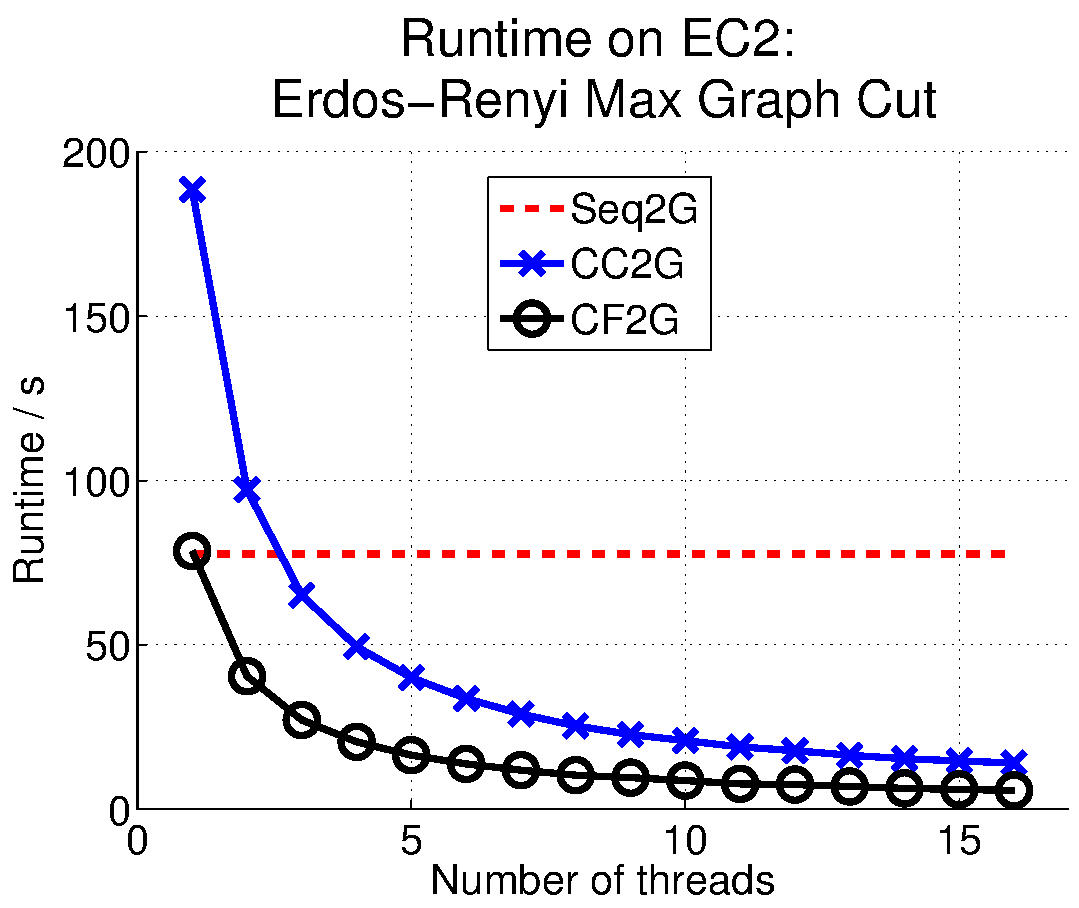
\includegraphics[width=110pt]{images/runtime_bigsynthetic_maxgraphcut.pdf}
			\caption{}
			\label{appfig:runtime_bigsynthetic_maxgraphcut}
	  \end{subfigure} &
	  \begin{subfigure}[b]{0.22\textwidth}
	  	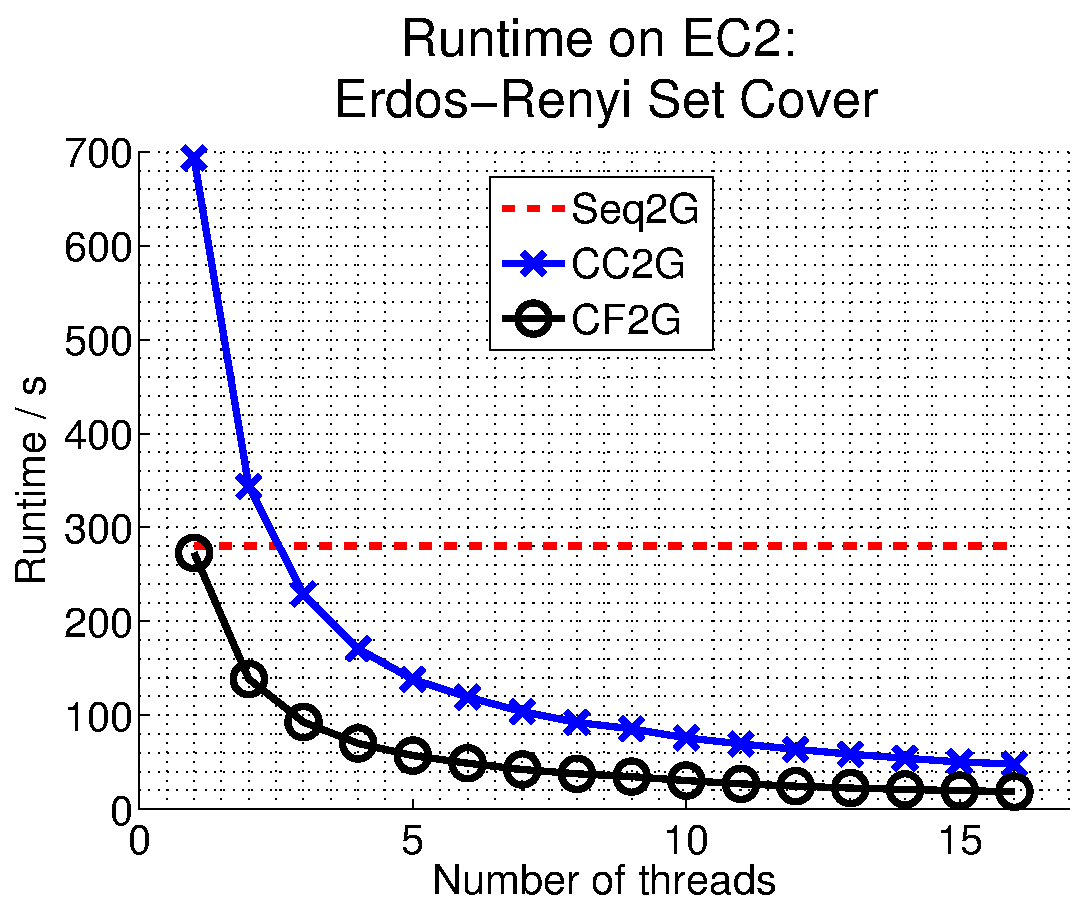
\includegraphics[width=110pt]{images/runtime_bigsynthetic_setcover.pdf}
			\caption{}
			\label{appfig:runtime_bigsynthetic_setcover}
	  \end{subfigure} &
	  \begin{subfigure}[b]{0.22\textwidth}
	  	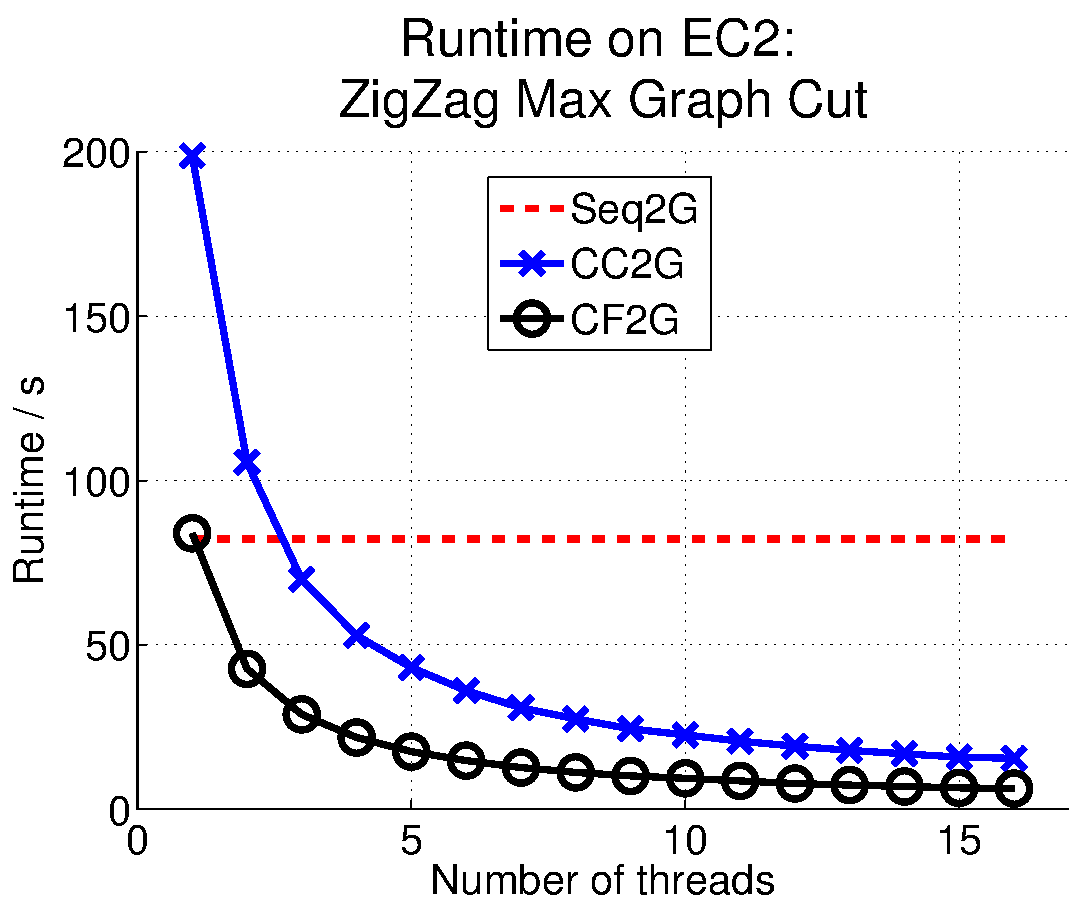
\includegraphics[width=110pt]{images/runtime_zigzag_maxgraphcut.pdf}
			\caption{}
			\label{appfig:runtime_zigzag_maxgraphcut}
	  \end{subfigure} &
	  \begin{subfigure}[b]{0.22\textwidth}
	  	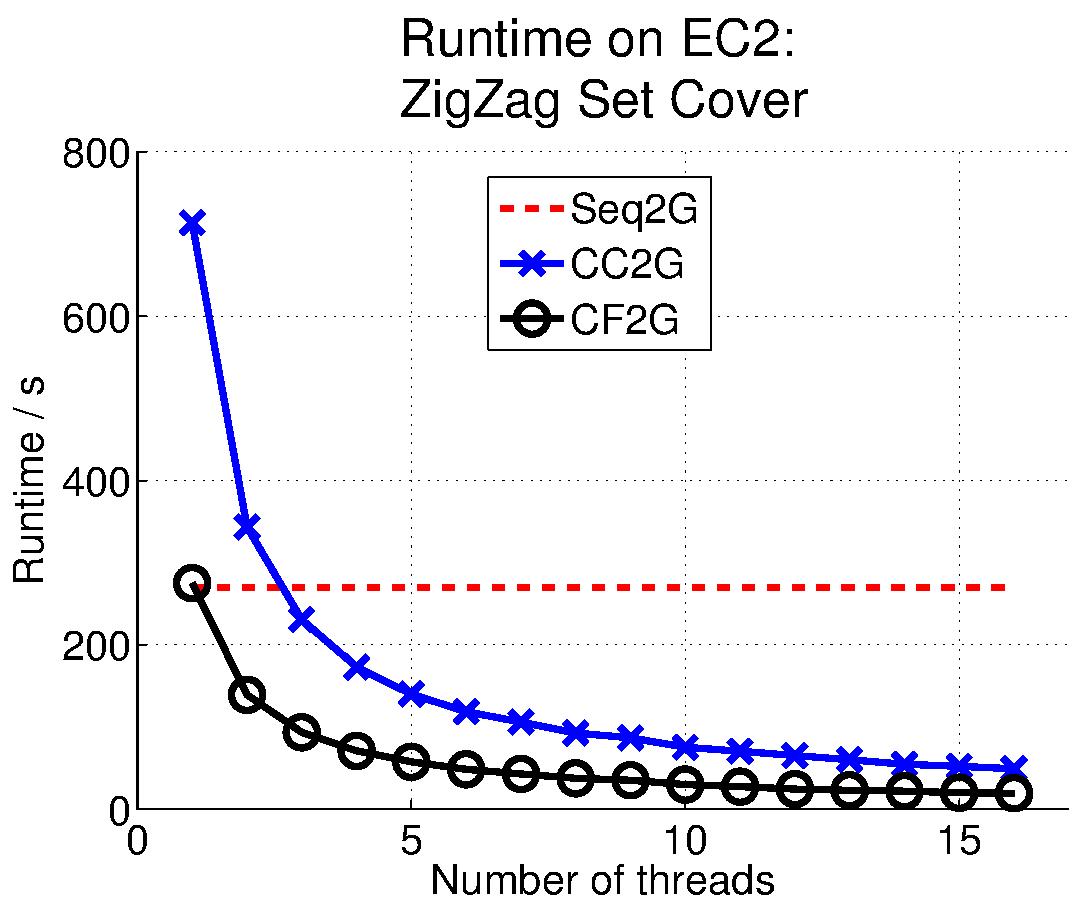
\includegraphics[width=110pt]{images/runtime_zigzag_setcover.pdf}
			\caption{}
			\label{appfig:runtime_zigzag_setcover}
	  \end{subfigure} \\
	  \begin{subfigure}[b]{0.22\textwidth}
	  	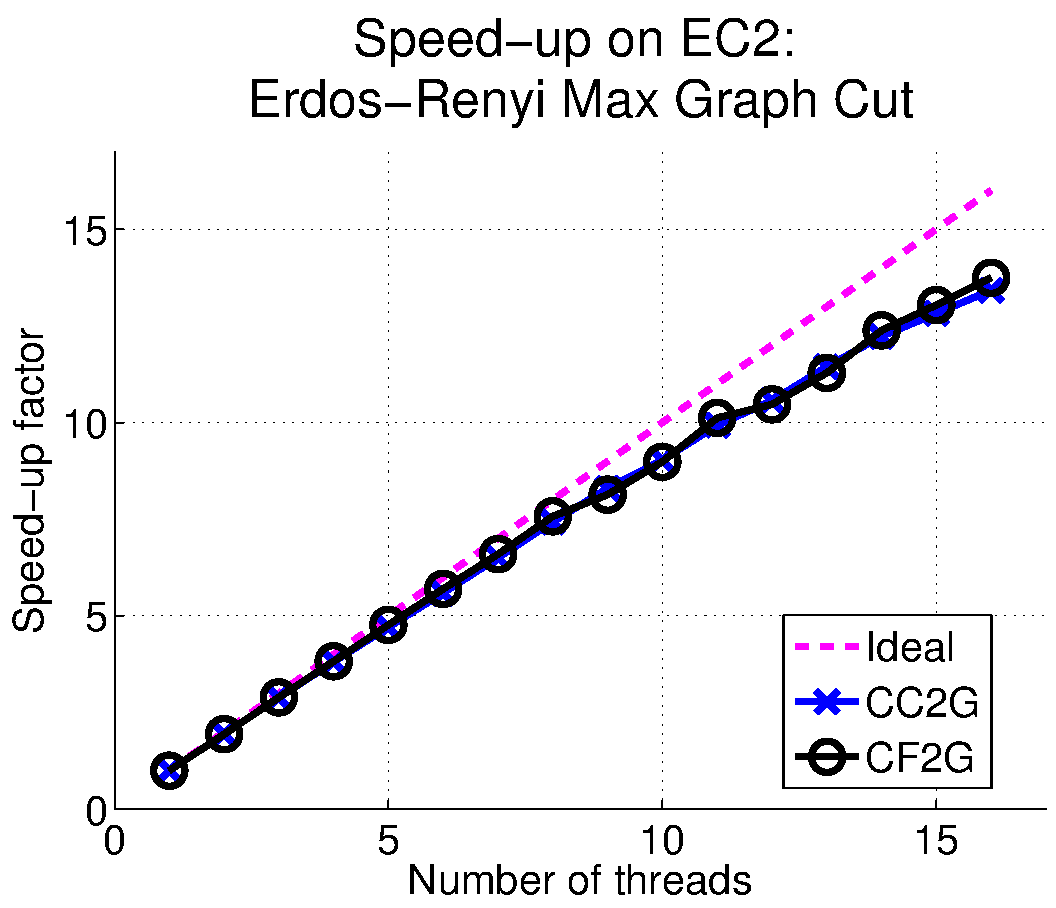
\includegraphics[width=110pt]{images/speedup_bigsynthetic_maxgraphcut.pdf}
			\caption{}
			\label{appfig:speedup_bigsynthetic_maxgraphcut}
	  \end{subfigure} &
	  \begin{subfigure}[b]{0.22\textwidth}
	  	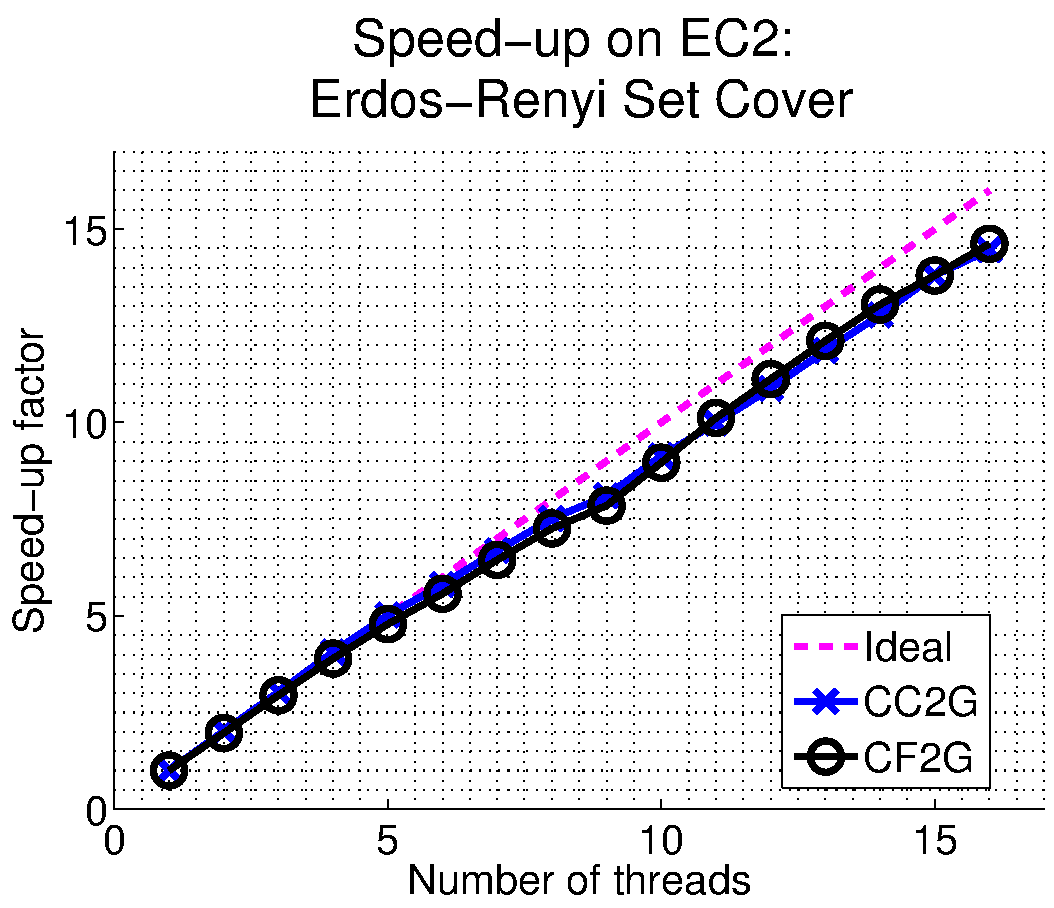
\includegraphics[width=110pt]{images/speedup_bigsynthetic_setcover.pdf}
			\caption{}
			\label{appfig:speedup_bigsynthetic_setcover}
	  \end{subfigure} &
	  \begin{subfigure}[b]{0.22\textwidth}
	  	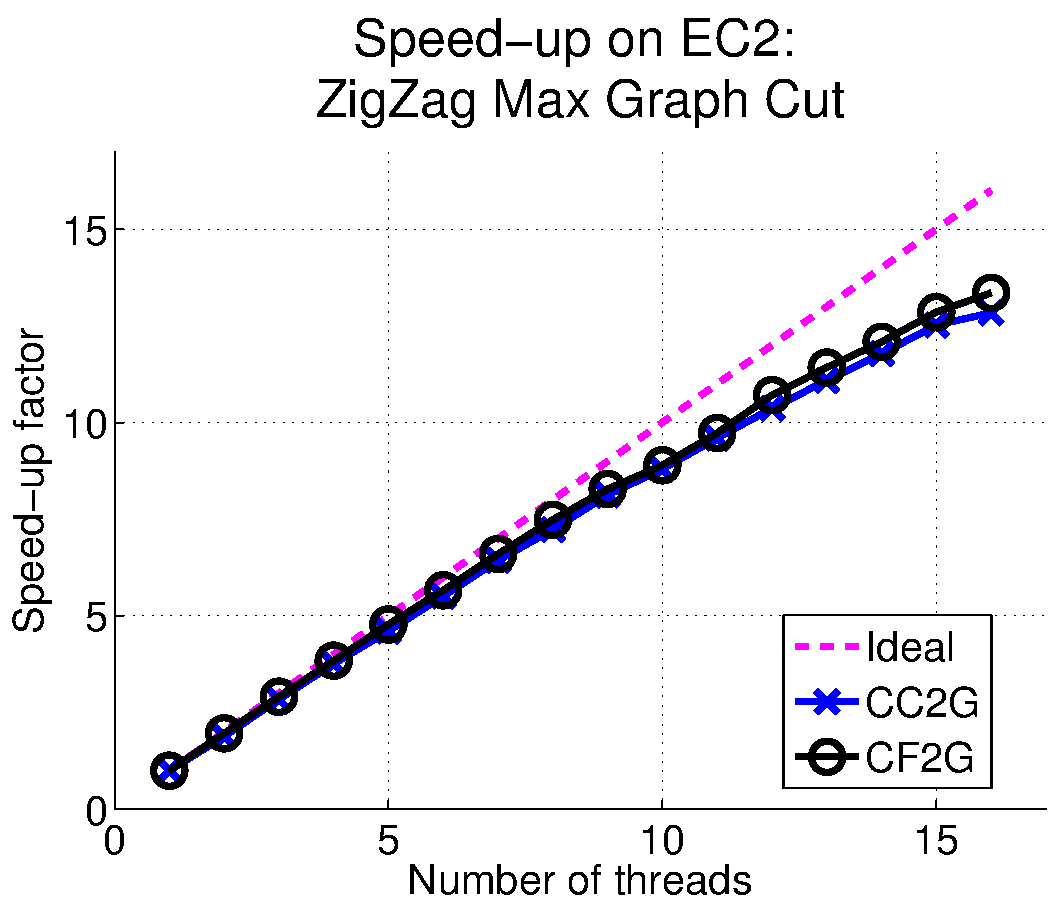
\includegraphics[width=110pt]{images/speedup_zigzag_maxgraphcut.pdf}
			\caption{}
			\label{appfig:speedup_zigzag_maxgraphcut}
	  \end{subfigure} &
	  \begin{subfigure}[b]{0.22\textwidth}
	  	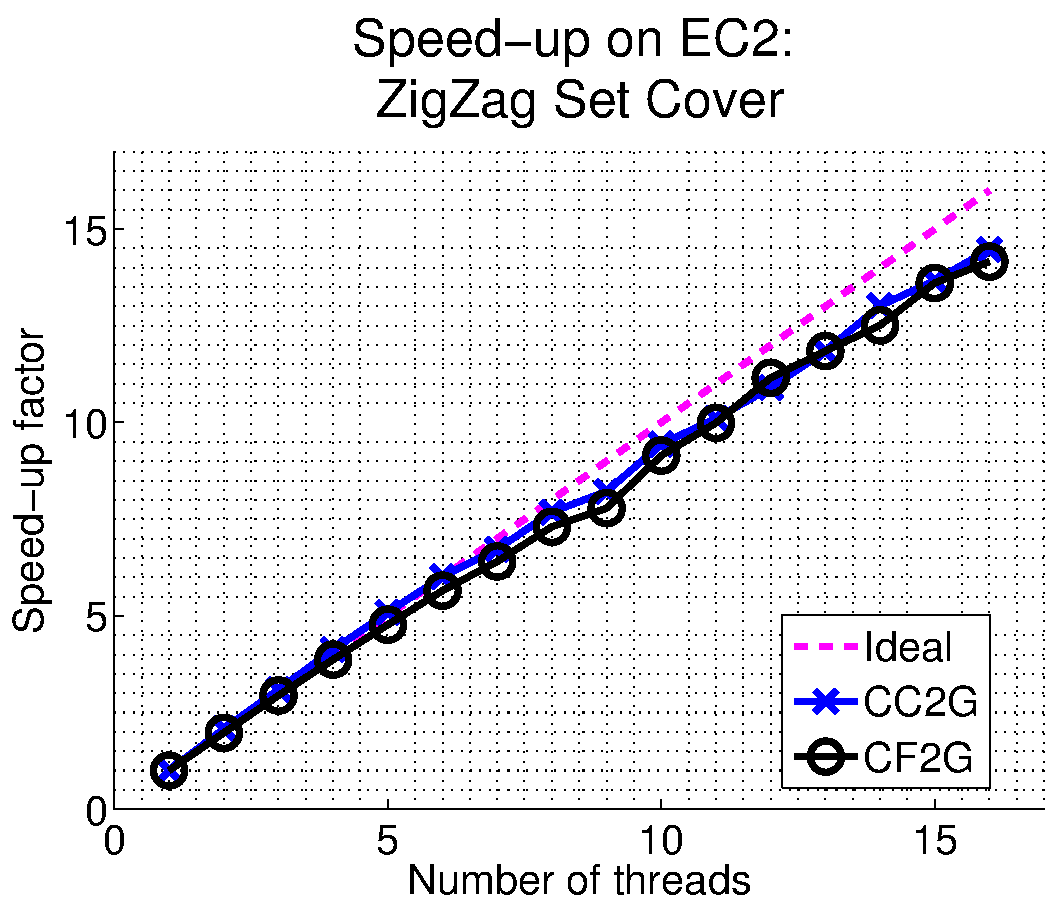
\includegraphics[width=110pt]{images/speedup_zigzag_setcover.pdf}
			\caption{}
			\label{appfig:speedup_zigzag_setcover}
	  \end{subfigure} \\
	  \begin{subfigure}[b]{0.22\textwidth}
	  	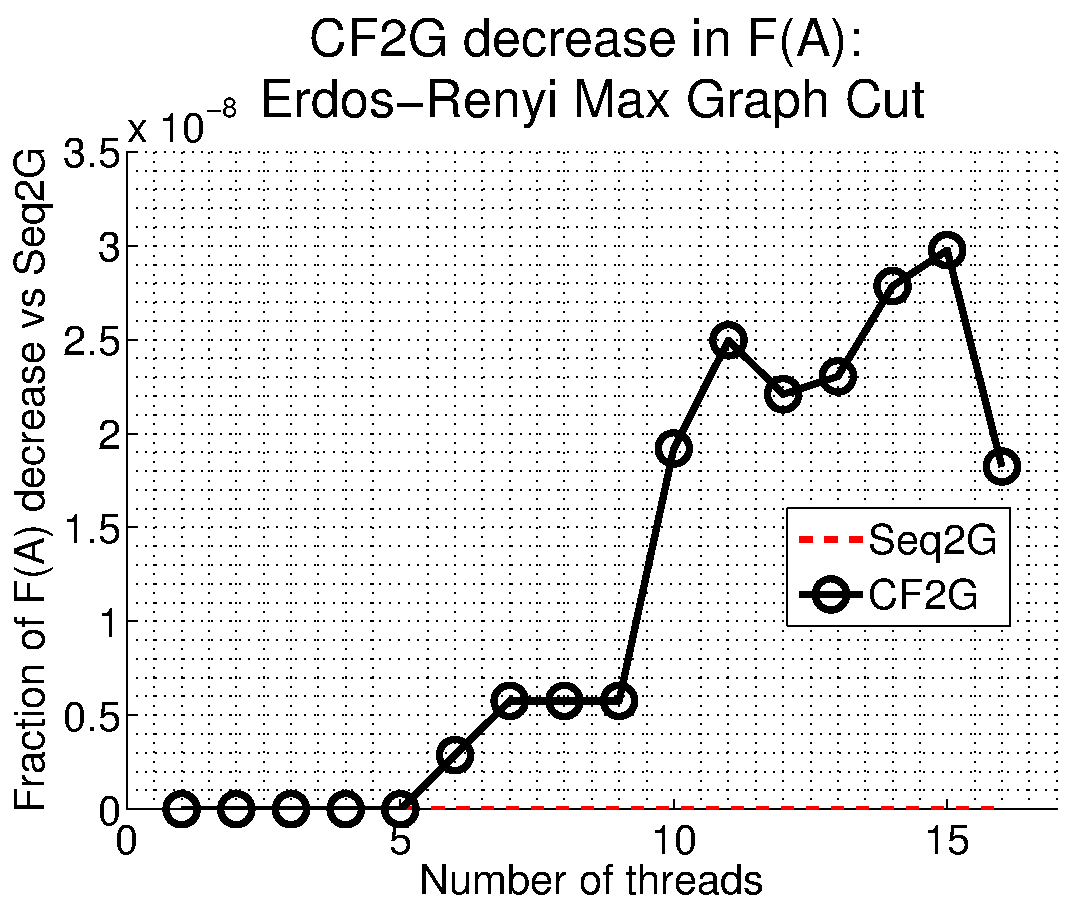
\includegraphics[width=110pt]{images/diffFA_CF2G_bigsynthetic_maxgraphcut.pdf}
			\caption{}
			\label{appfig:diffFA_CF2G_bigsynthetic_maxgraphcut}
	  \end{subfigure} &
	  \begin{subfigure}[b]{0.22\textwidth}
	  	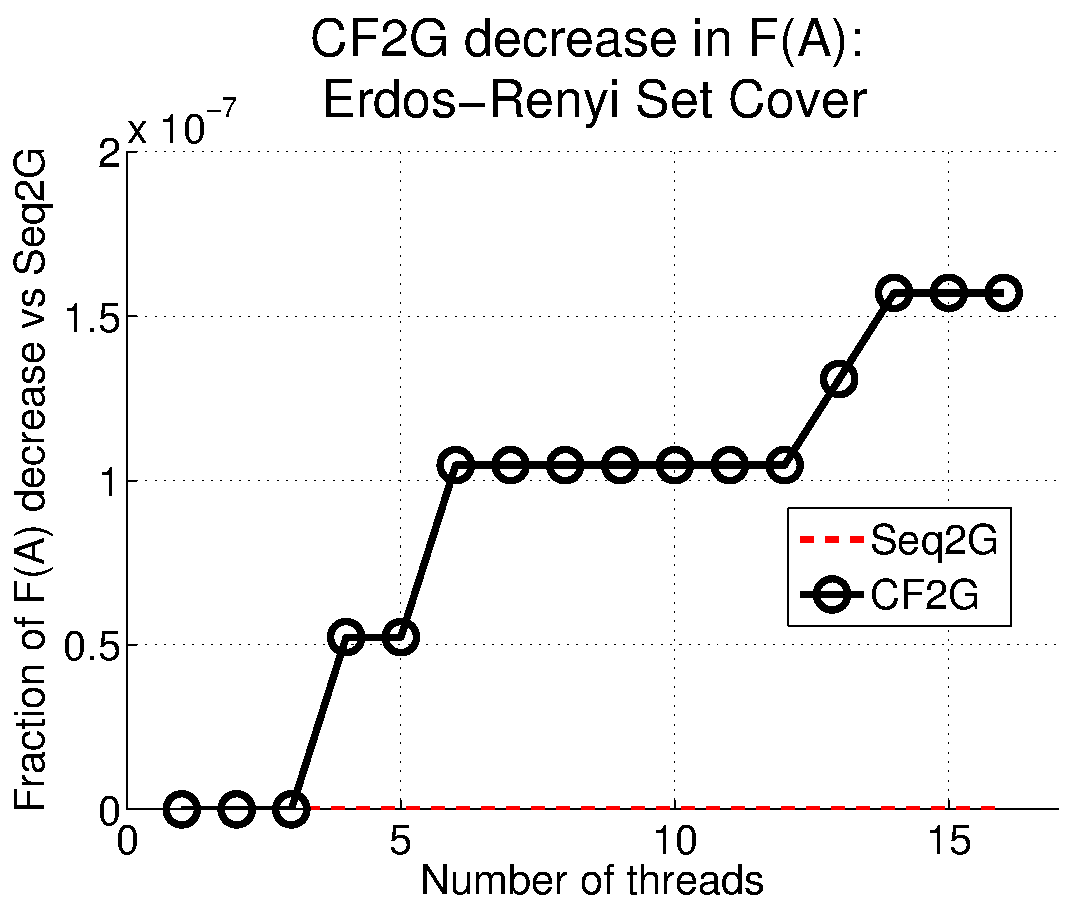
\includegraphics[width=110pt]{images/diffFA_CF2G_bigsynthetic_setcover.pdf}
			\caption{}
			\label{appfig:diffFA_CF2G_bigsynthetic_setcover}
	  \end{subfigure} &
	  \begin{subfigure}[b]{0.22\textwidth}
	  	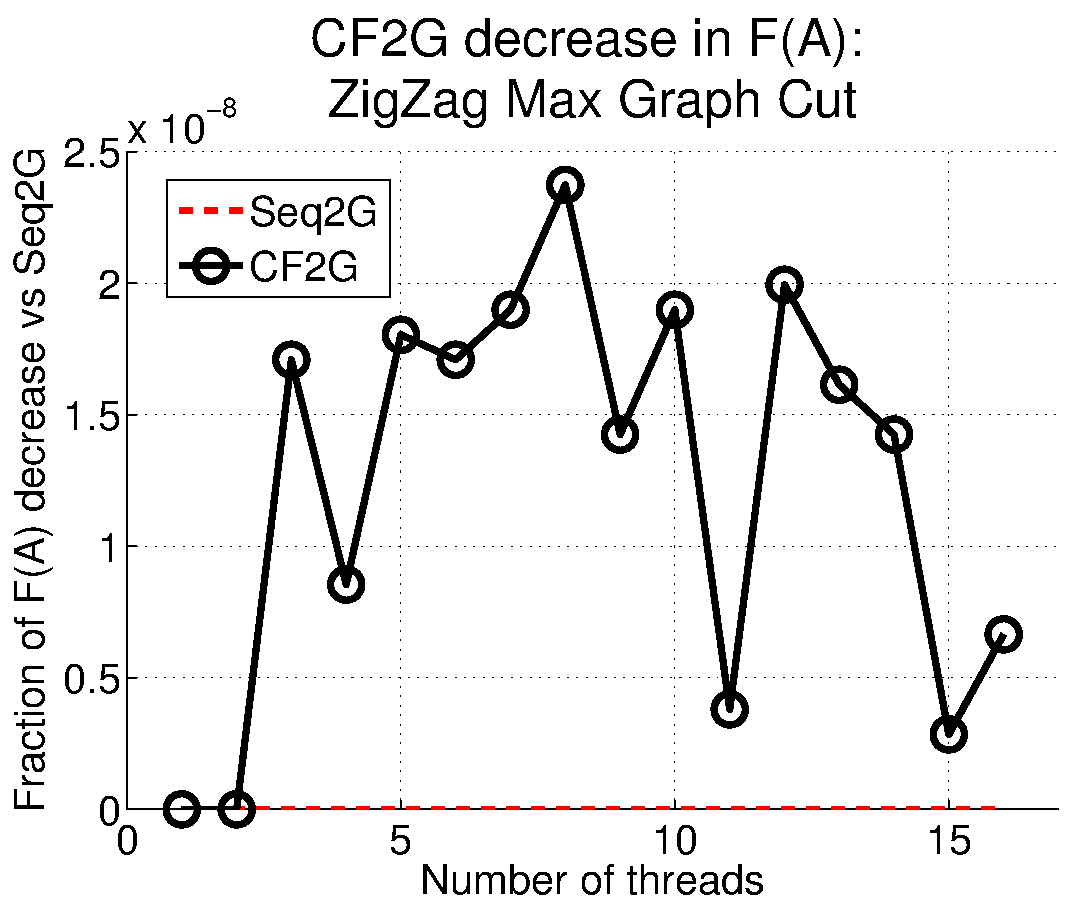
\includegraphics[width=110pt]{images/diffFA_CF2G_zigzag_maxgraphcut.pdf}
			\caption{}
			\label{appfig:diffFA_CF2G_zigzag_maxgraphcut}
	  \end{subfigure} &
	  \begin{subfigure}[b]{0.22\textwidth}
	  	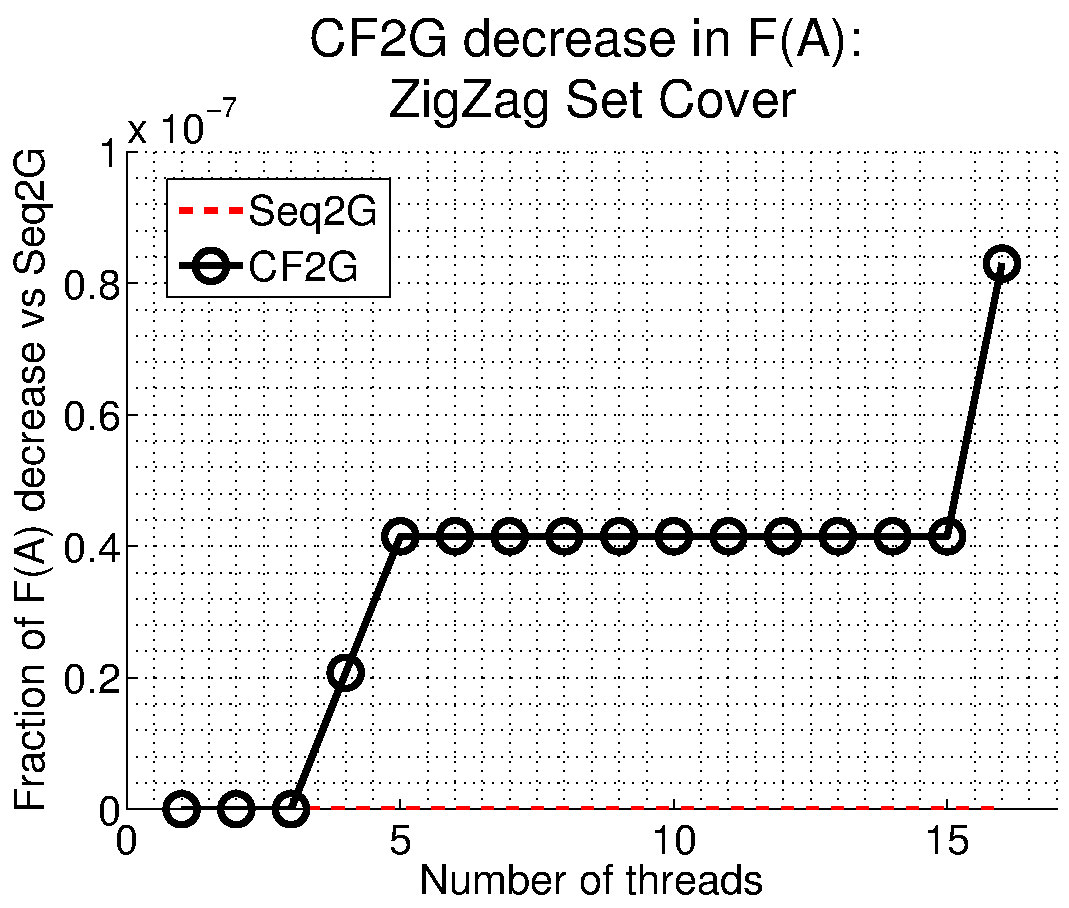
\includegraphics[width=110pt]{images/diffFA_CF2G_zigzag_setcover.pdf}
			\caption{}
			\label{appfig:diffFA_CF2G_zigzag_setcover}
	  \end{subfigure} \\
	  \begin{subfigure}[b]{0.22\textwidth}
	  	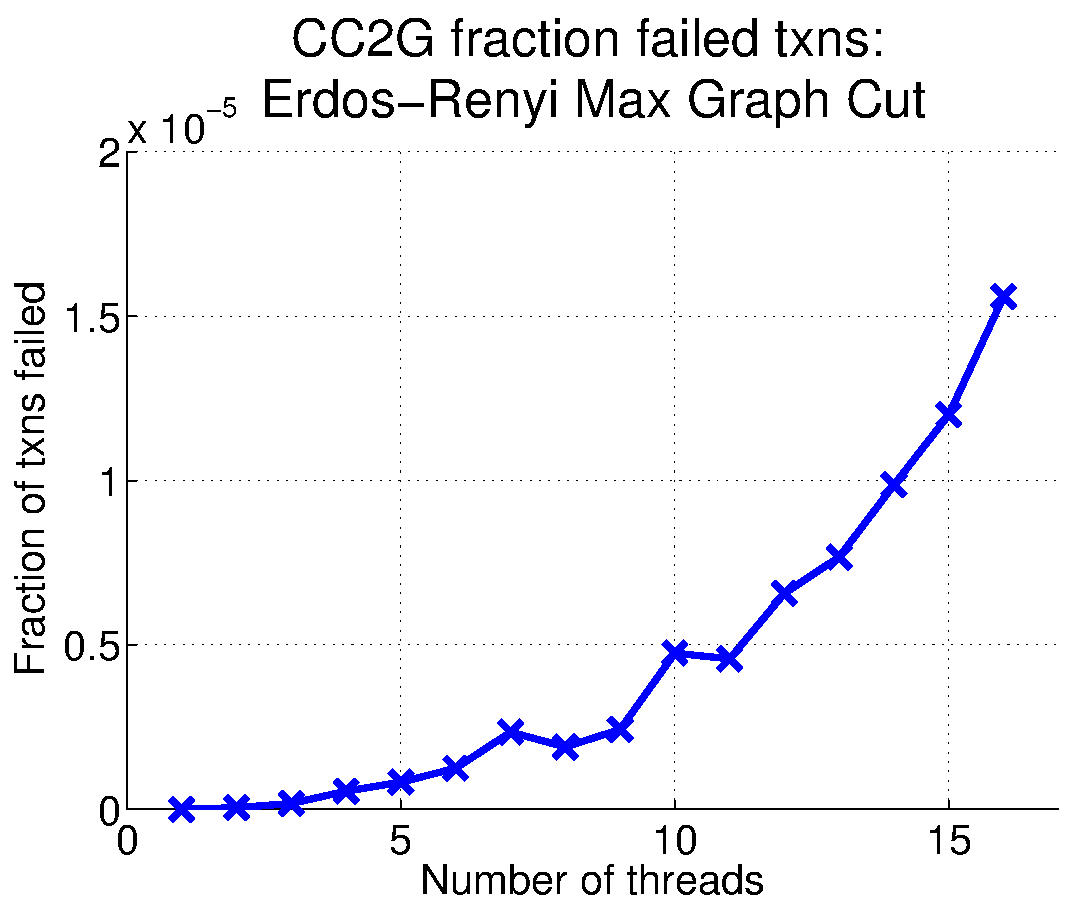
\includegraphics[width=110pt]{images/validated_CC2G_bigsynthetic_maxgraphcut.pdf}
			\caption{}
			\label{appfig:validated_CC2G_bigsynthetic_maxgraphcut}
	  \end{subfigure} &
	  \begin{subfigure}[b]{0.22\textwidth}
	  	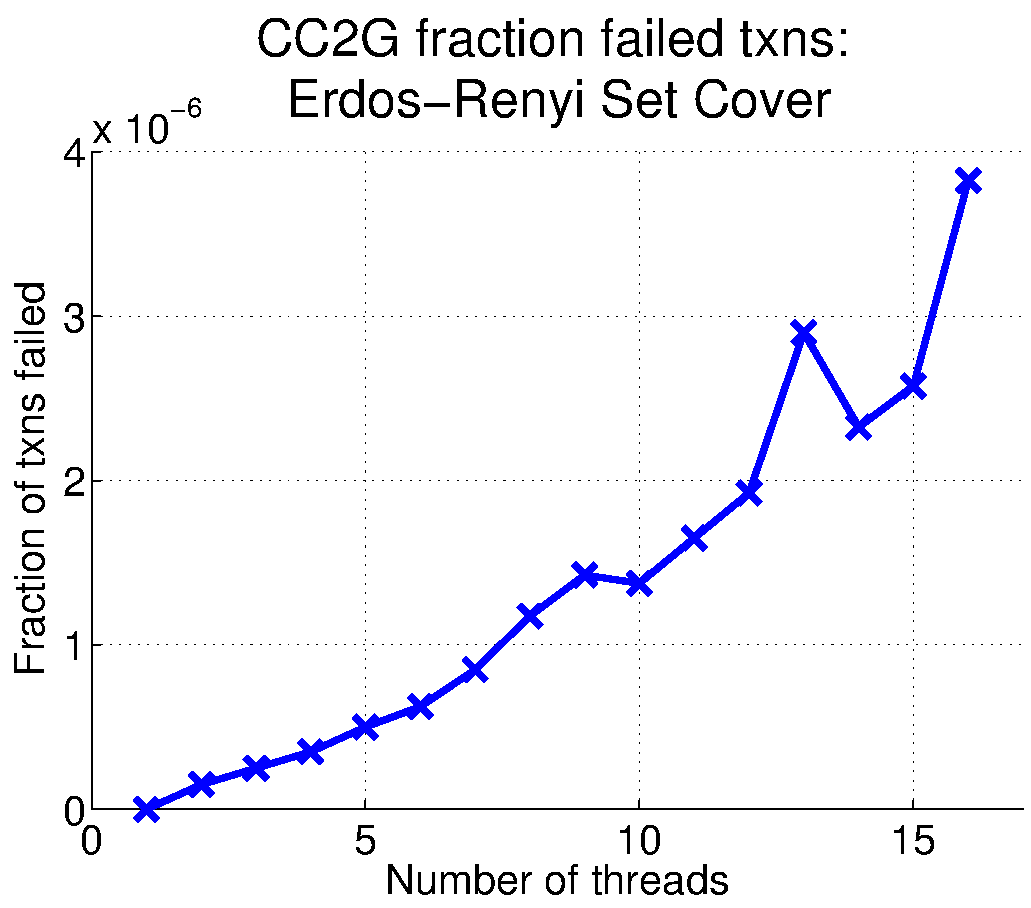
\includegraphics[width=110pt]{images/validated_CC2G_bigsynthetic_setcover.pdf}
			\caption{}
			\label{appfig:validated_CC2G_bigsynthetic_setcover}
	  \end{subfigure} &
	  \begin{subfigure}[b]{0.22\textwidth}
	  	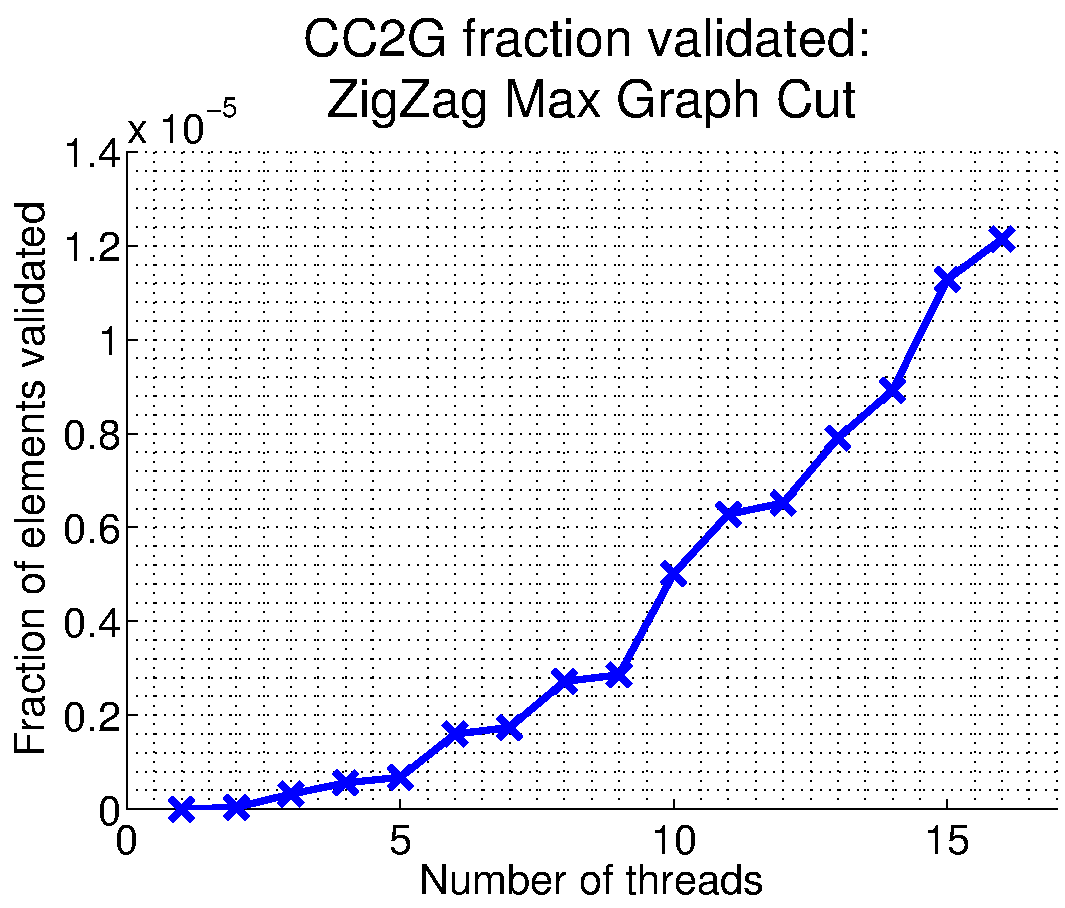
\includegraphics[width=110pt]{images/validated_CC2G_zigzag_maxgraphcut.pdf}
			\caption{}
			\label{appfig:validated_CC2G_zigzag_maxgraphcut}
	  \end{subfigure} &
	  \begin{subfigure}[b]{0.22\textwidth}
	  	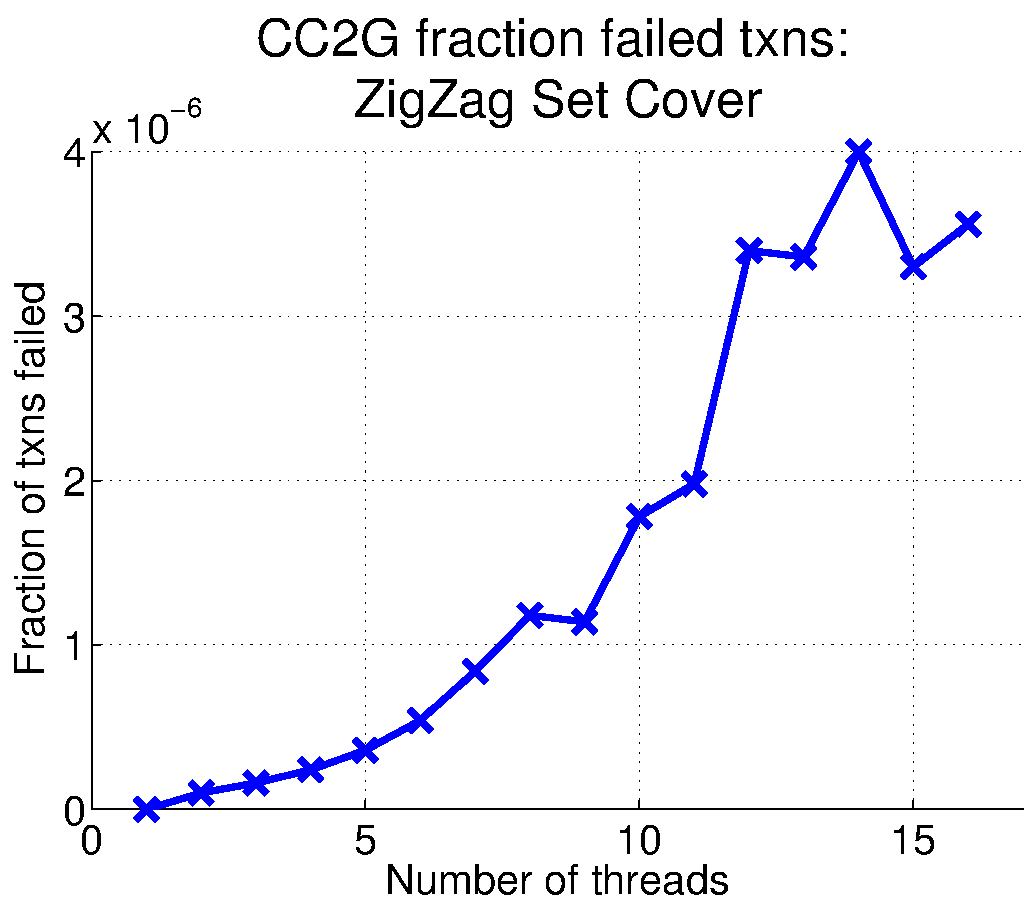
\includegraphics[width=110pt]{images/validated_CC2G_zigzag_setcover.pdf}
			\caption{}
			\label{appfig:validated_CC2G_zigzag_setcover}
	  \end{subfigure} \\
  \end{tabular}
  \caption{Experimental results on Erdos-Renyi and ZigZag synthetic graphs.}
\end{figure}


~\newpage\begin{figure}[ht]
  \centering
  \begin{tabular}{cccc}
	  \begin{subfigure}[b]{0.22\textwidth}
	  	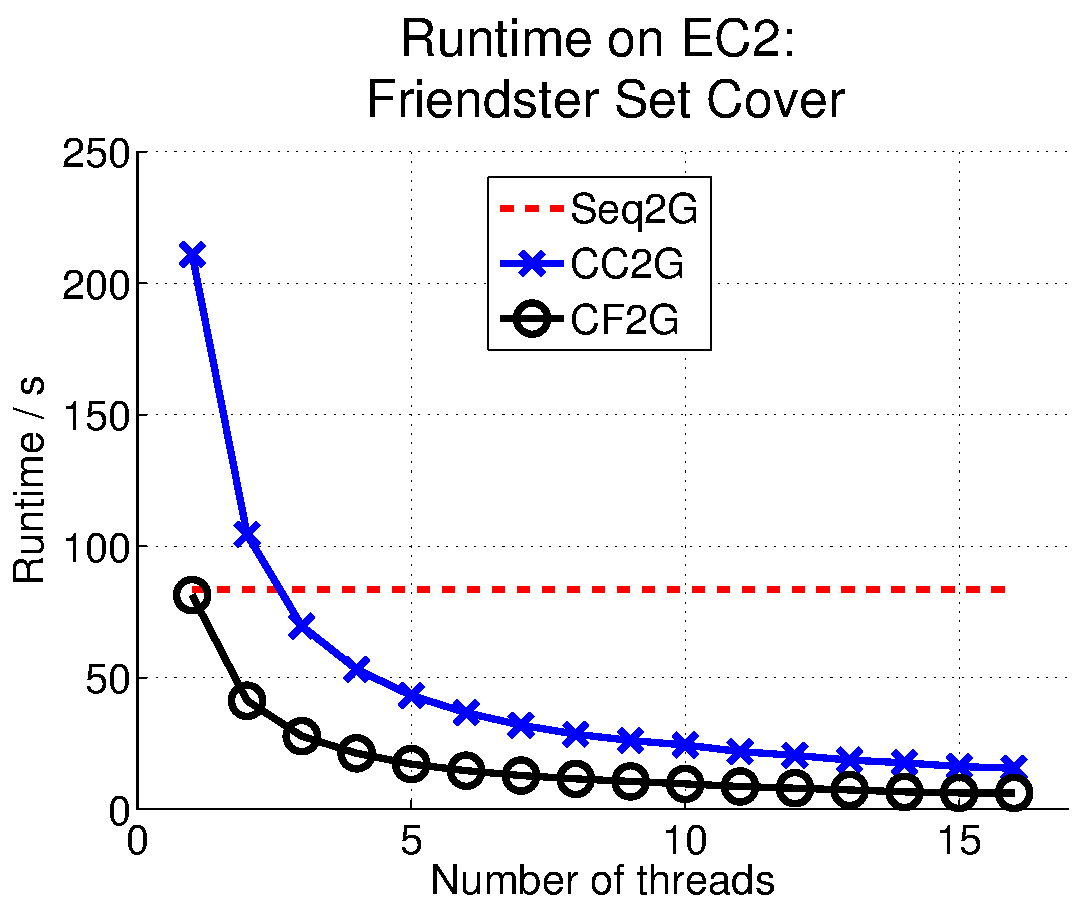
\includegraphics[width=110pt]{images/runtime_friendster10M_setcover.pdf}
			\caption{}
			\label{appfig:runtime_friendster10M_setcover}
	  \end{subfigure} &
	  \begin{subfigure}[b]{0.22\textwidth}
	  	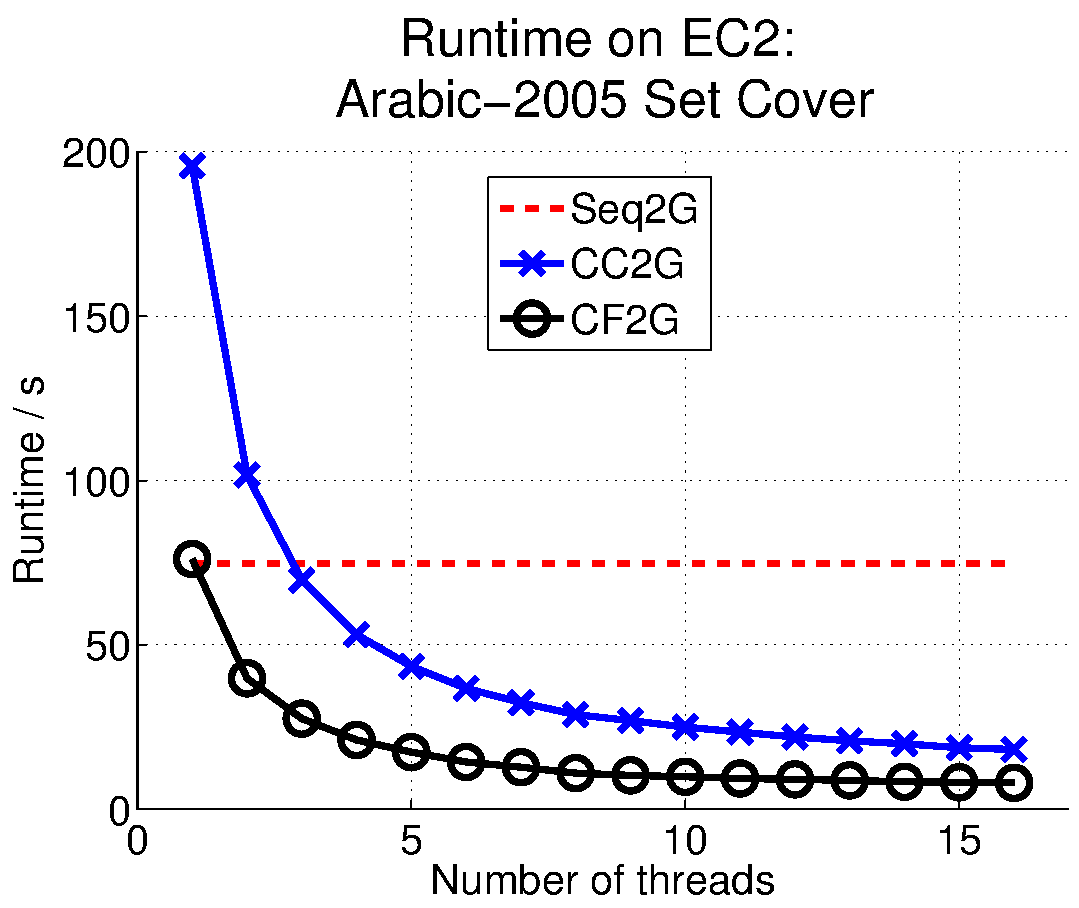
\includegraphics[width=110pt]{images/runtime_arabic2005_setcover.pdf}
			\caption{}
			\label{appfig:runtime_arabic2005_setcover}
	  \end{subfigure} &
	  \begin{subfigure}[b]{0.22\textwidth}
	  	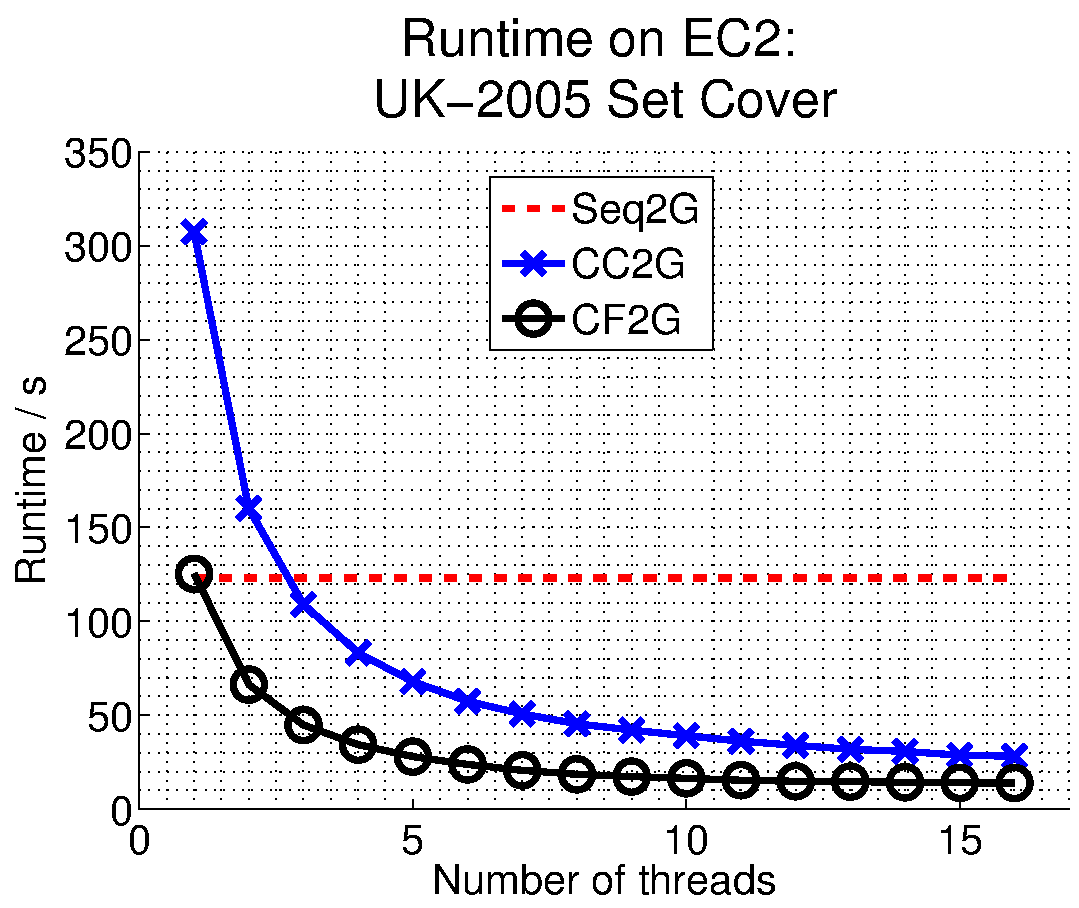
\includegraphics[width=110pt]{images/runtime_uk2005_setcover.pdf}
			\caption{}
			\label{appfig:runtime_uk2005_setcover}
	  \end{subfigure} &
	  \begin{subfigure}[b]{0.22\textwidth}
	  	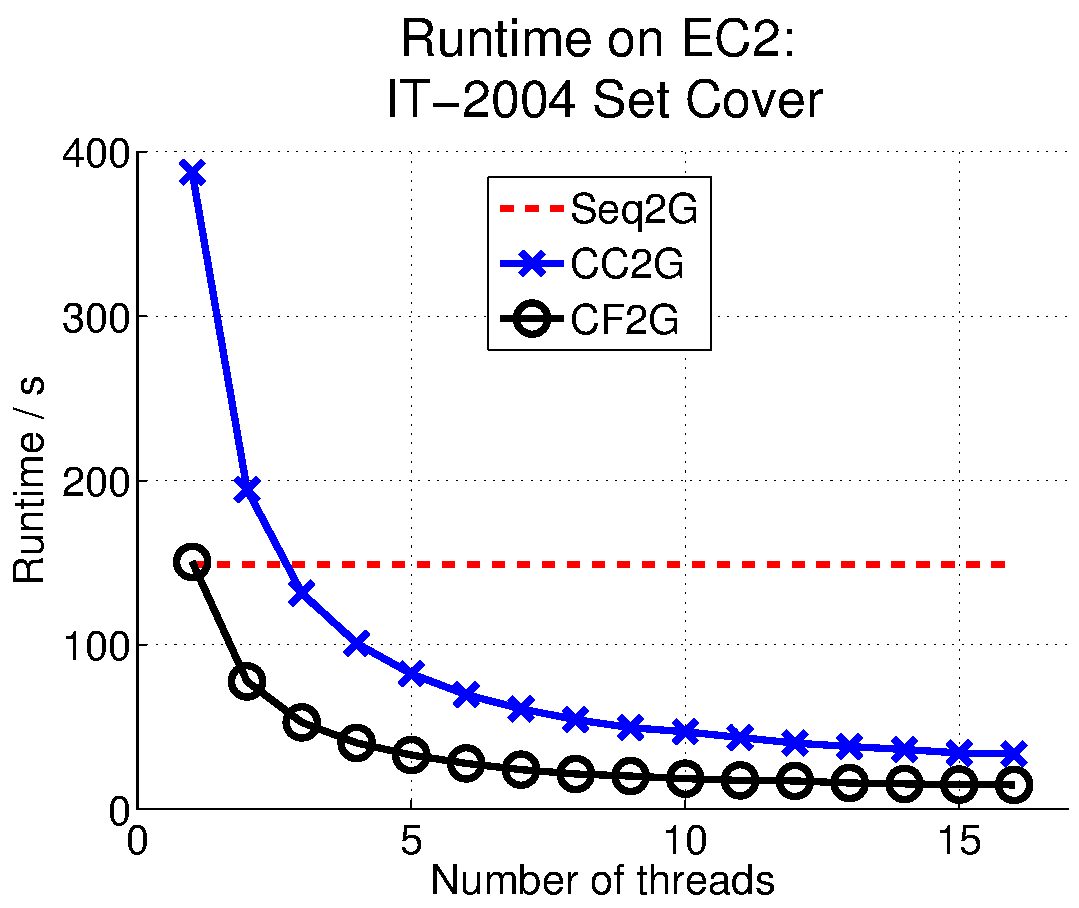
\includegraphics[width=110pt]{images/runtime_it2004_setcover.pdf}
			\caption{}
			\label{appfig:runtime_it2004_setcover}
	  \end{subfigure} \\
	  \begin{subfigure}[b]{0.22\textwidth}
	  	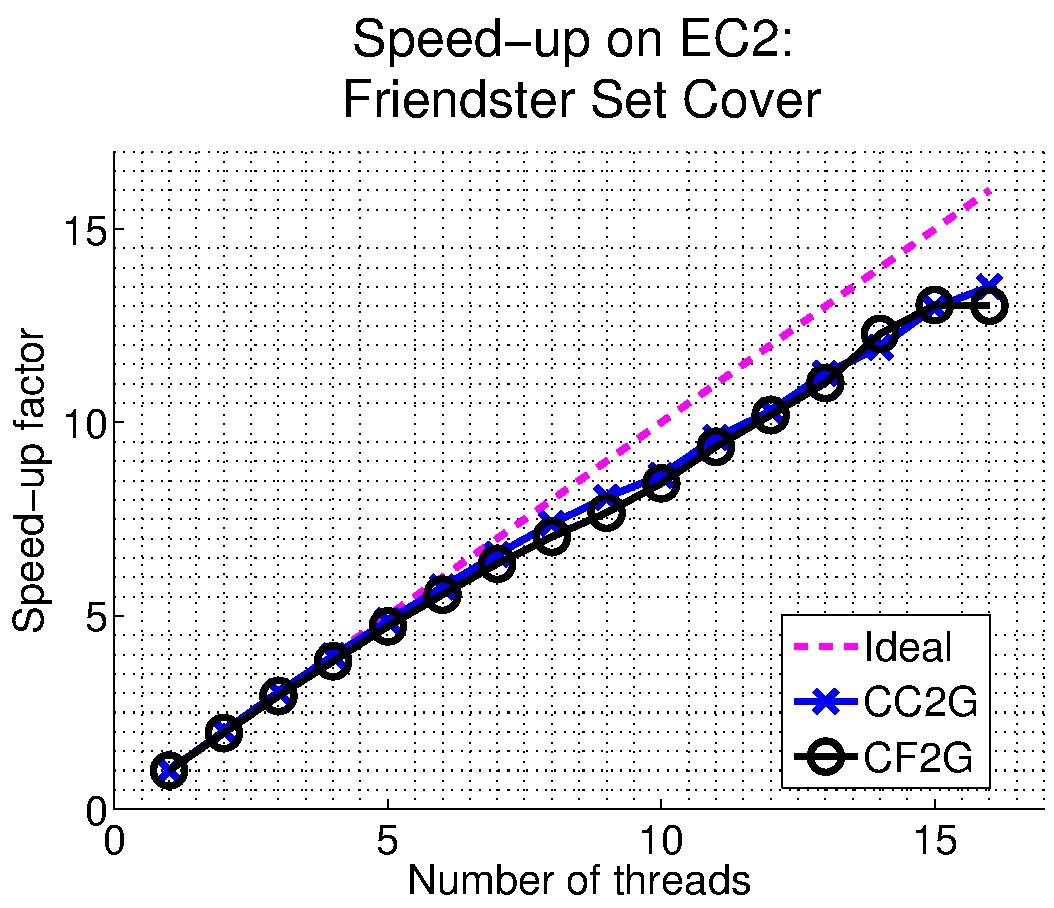
\includegraphics[width=110pt]{images/speedup_friendster10M_setcover.pdf}
			\caption{}
			\label{appfig:speedup_friendster10M_setcover}
	  \end{subfigure} &
	  \begin{subfigure}[b]{0.22\textwidth}
	  	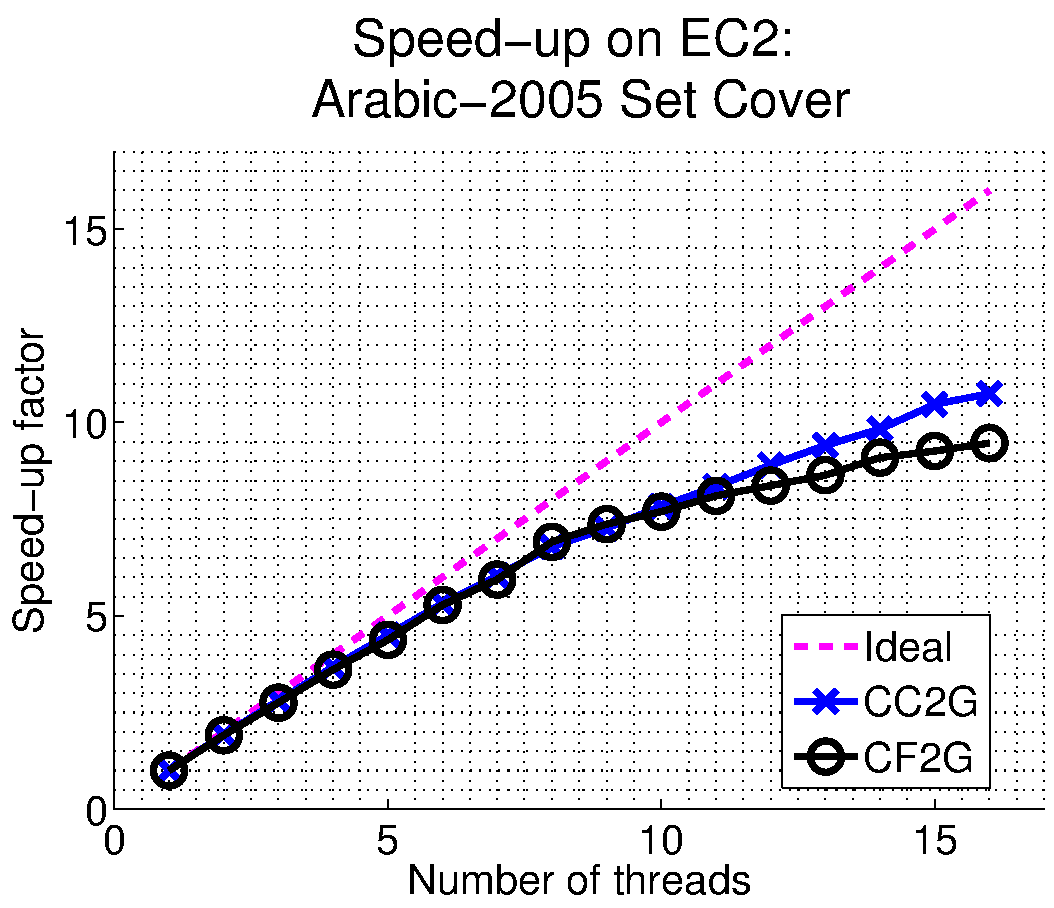
\includegraphics[width=110pt]{images/speedup_arabic2005_setcover.pdf}
			\caption{}
			\label{appfig:speedup_arabic2005_setcover}
	  \end{subfigure} &
	  \begin{subfigure}[b]{0.22\textwidth}
	  	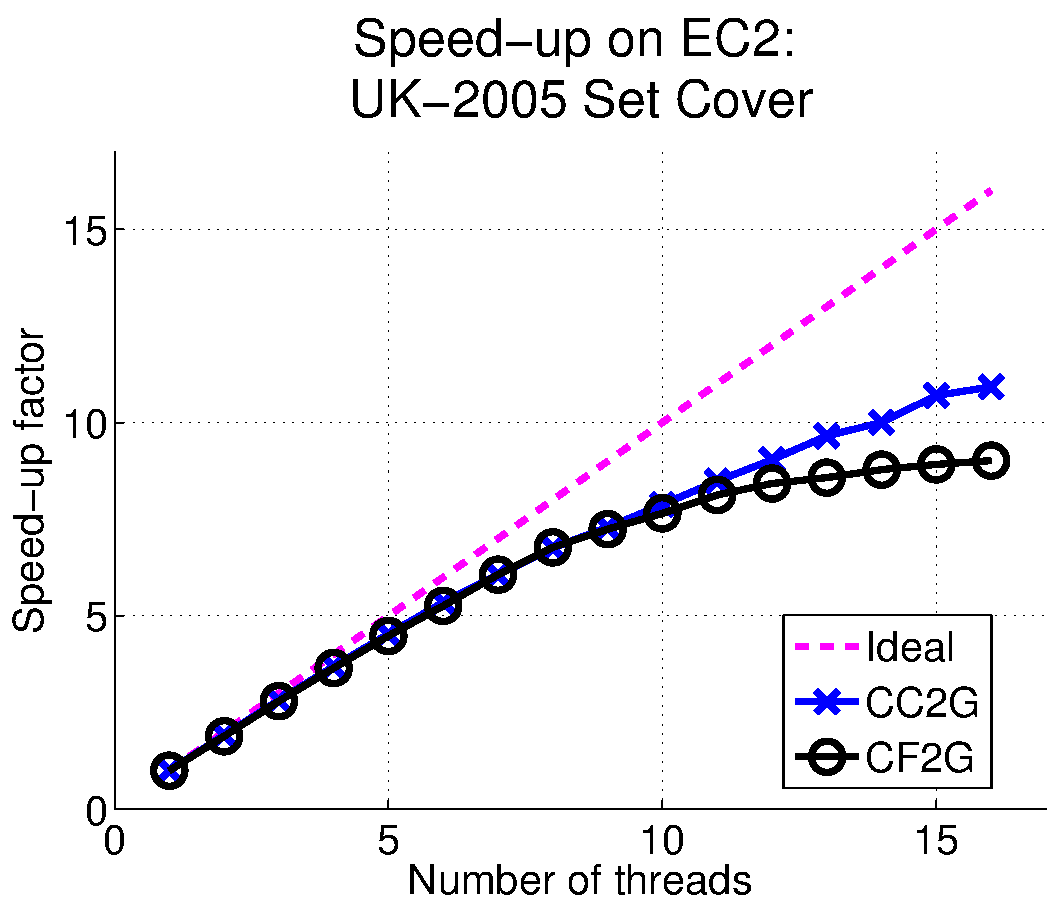
\includegraphics[width=110pt]{images/speedup_uk2005_setcover.pdf}
			\caption{}
			\label{appfig:speedup_uk2005_setcover}
	  \end{subfigure} &
	  \begin{subfigure}[b]{0.22\textwidth}
	  	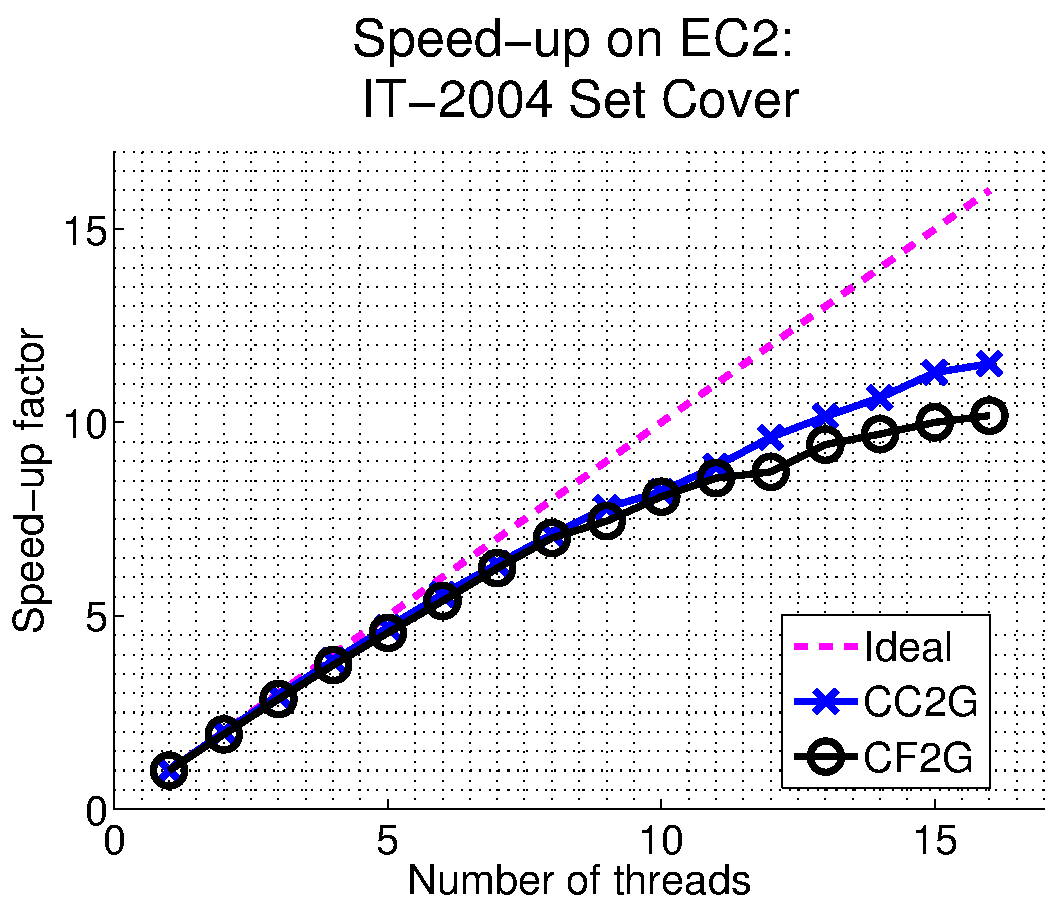
\includegraphics[width=110pt]{images/speedup_it2004_setcover.pdf}
			\caption{}
			\label{appfig:speedup_it2004_setcover}
	  \end{subfigure} \\
	  \begin{subfigure}[b]{0.22\textwidth}
	  	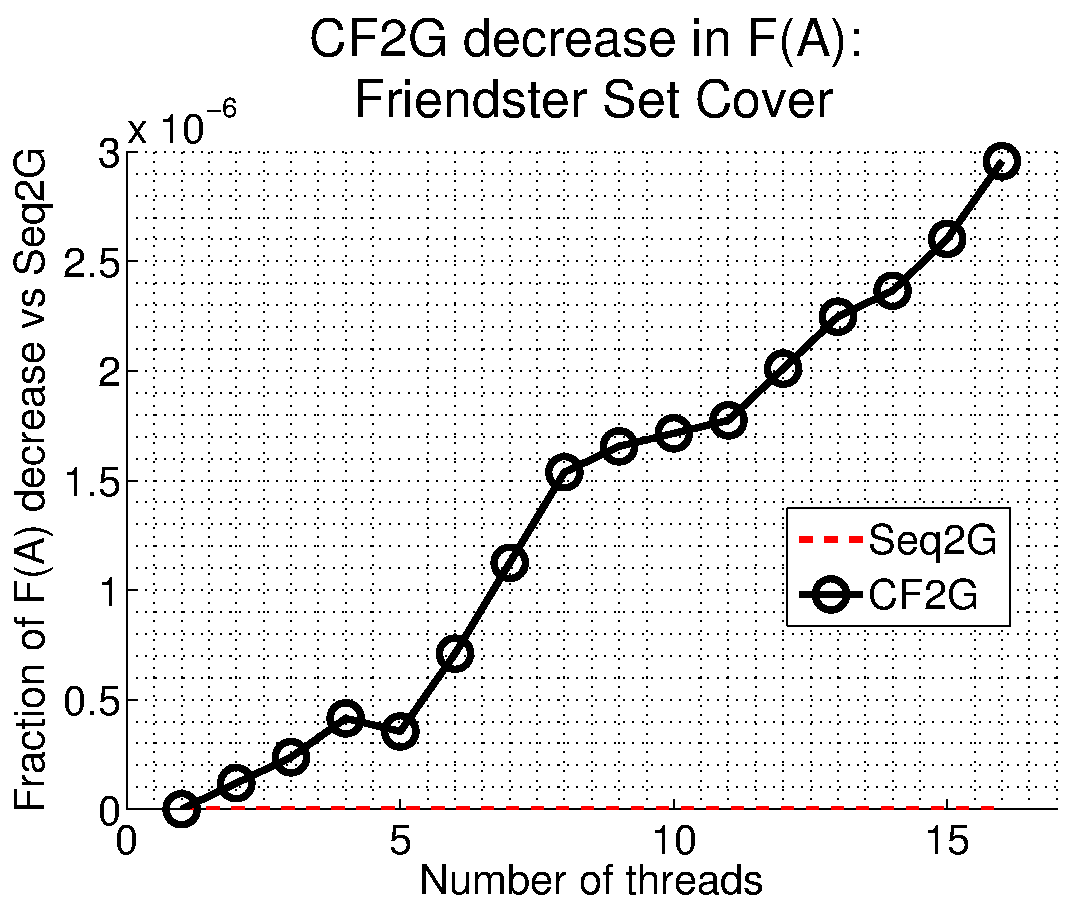
\includegraphics[width=110pt]{images/diffFA_CF2G_friendster10M_setcover.pdf}
			\caption{}
			\label{appfig:diffFA_CF2G_friendster10M_setcover}
	  \end{subfigure} &
	  \begin{subfigure}[b]{0.22\textwidth}
	  	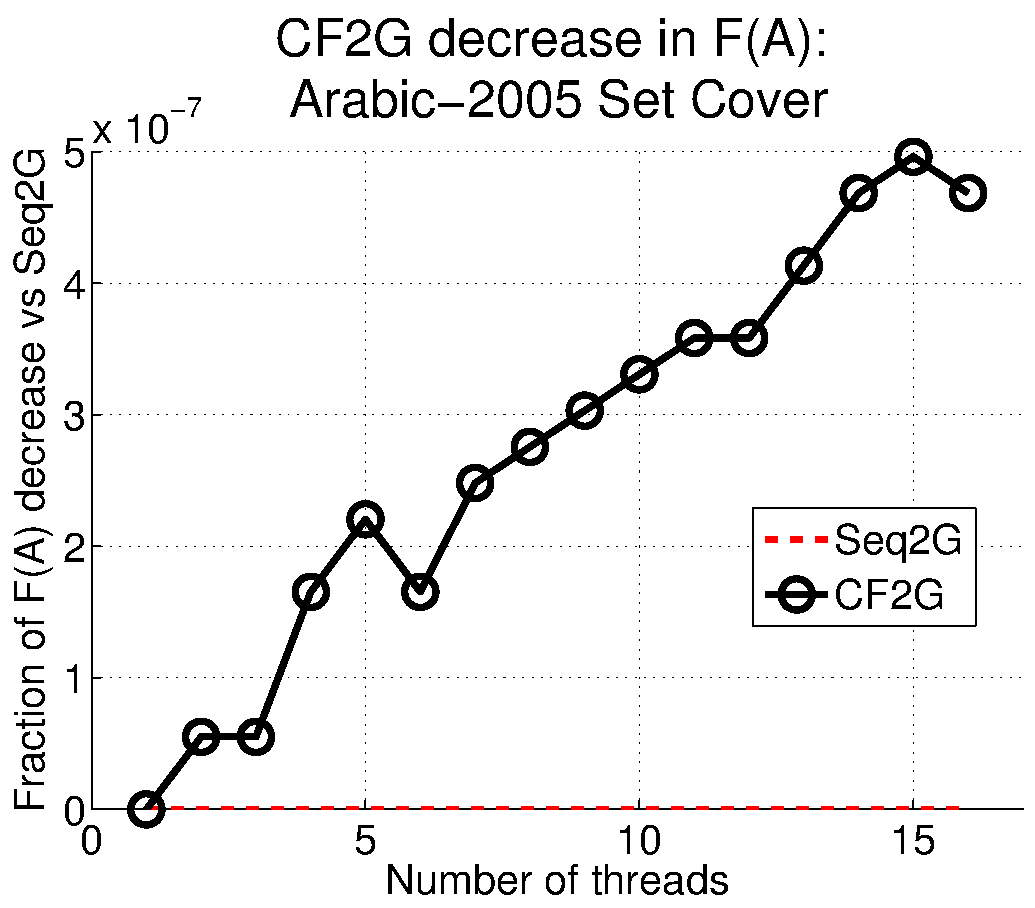
\includegraphics[width=110pt]{images/diffFA_CF2G_arabic2005_setcover.pdf}
			\caption{}
			\label{appfig:diffFA_CF2G_arabic2005_setcover}
	  \end{subfigure} &
	  \begin{subfigure}[b]{0.22\textwidth}
	  	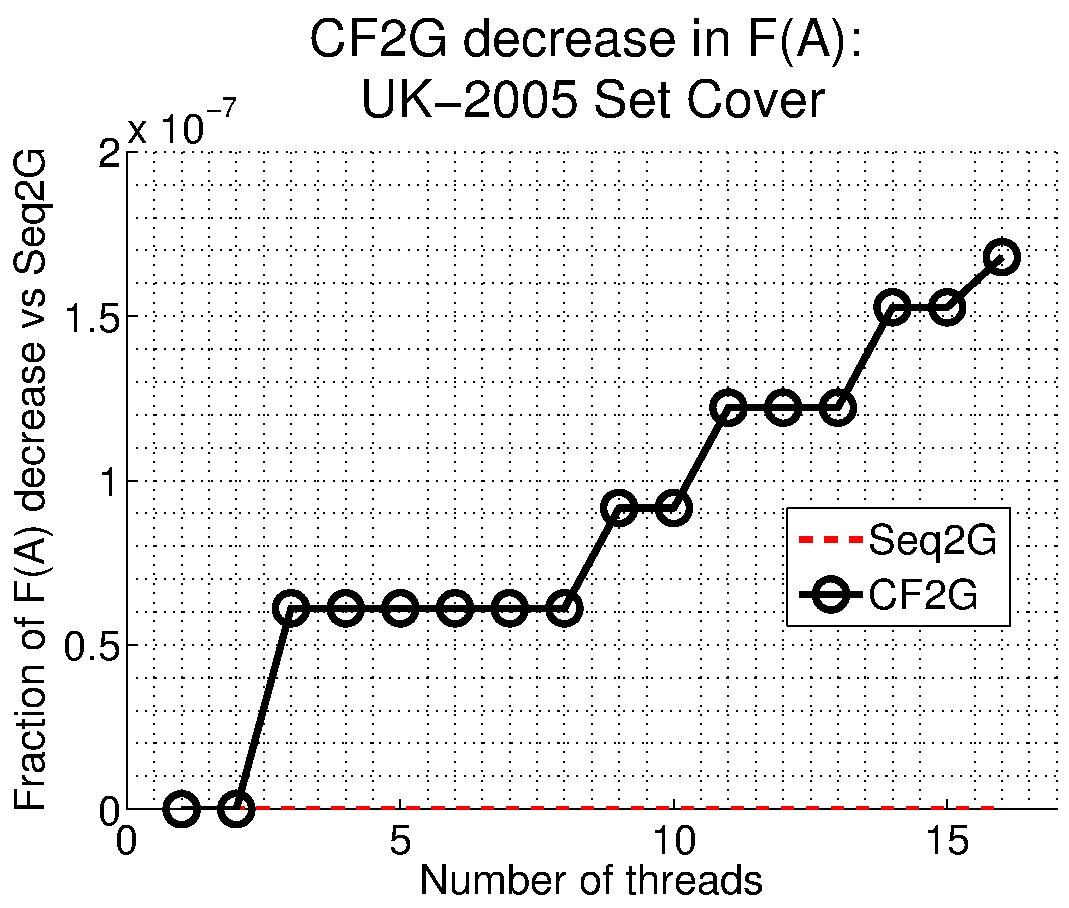
\includegraphics[width=110pt]{images/diffFA_CF2G_uk2005_setcover.pdf}
			\caption{}
			\label{appfig:diffFA_CF2G_uk2005_setcover}
	  \end{subfigure} &
	  \begin{subfigure}[b]{0.22\textwidth}
	  	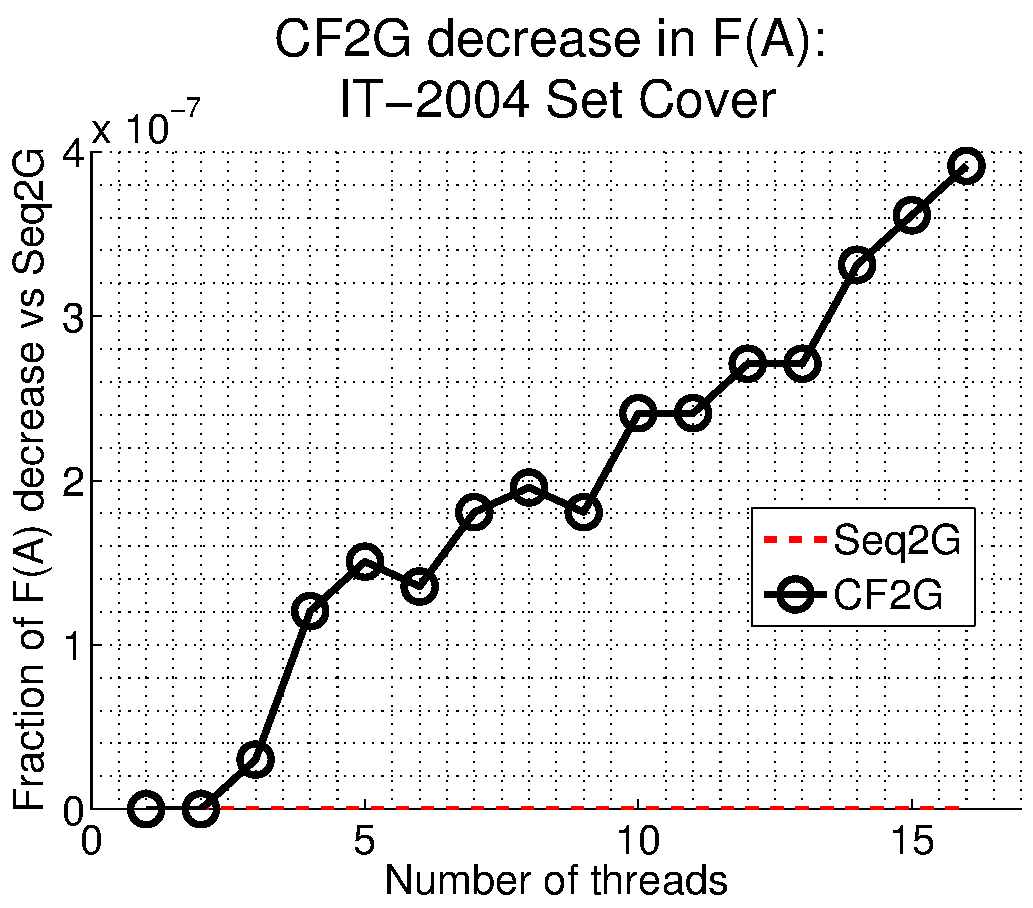
\includegraphics[width=110pt]{images/diffFA_CF2G_it2004_setcover.pdf}
			\caption{}
			\label{appfig:diffFA_CF2G_it2004_setcover}
	  \end{subfigure} \\
	  \begin{subfigure}[b]{0.22\textwidth}
	  	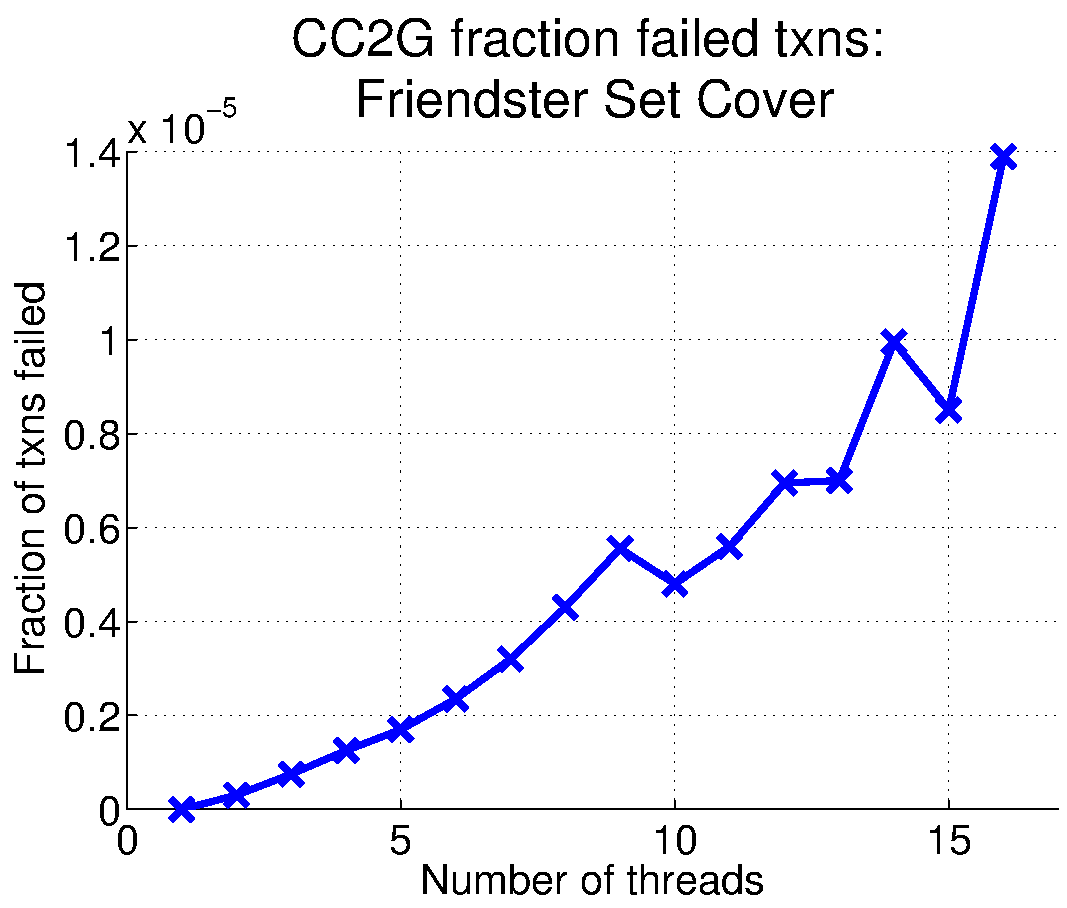
\includegraphics[width=110pt]{images/validated_CC2G_friendster10M_setcover.pdf}
			\caption{}
			\label{appfig:validated_CC2G_friendster10M_setcover}
	  \end{subfigure} &
	  \begin{subfigure}[b]{0.22\textwidth}
	  	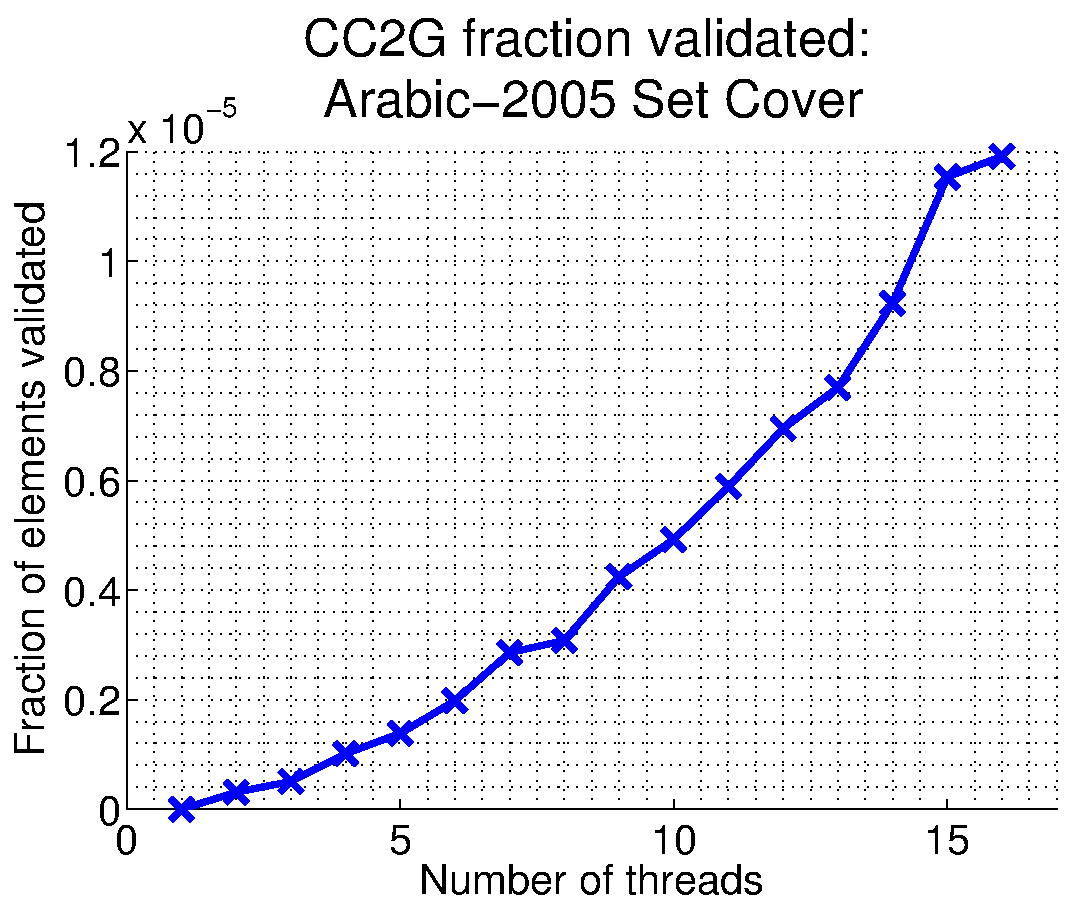
\includegraphics[width=110pt]{images/validated_CC2G_arabic2005_setcover.pdf}
			\caption{}
			\label{appfig:validated_CC2G_arabic2005_setcover}
	  \end{subfigure} &
	  \begin{subfigure}[b]{0.22\textwidth}
	  	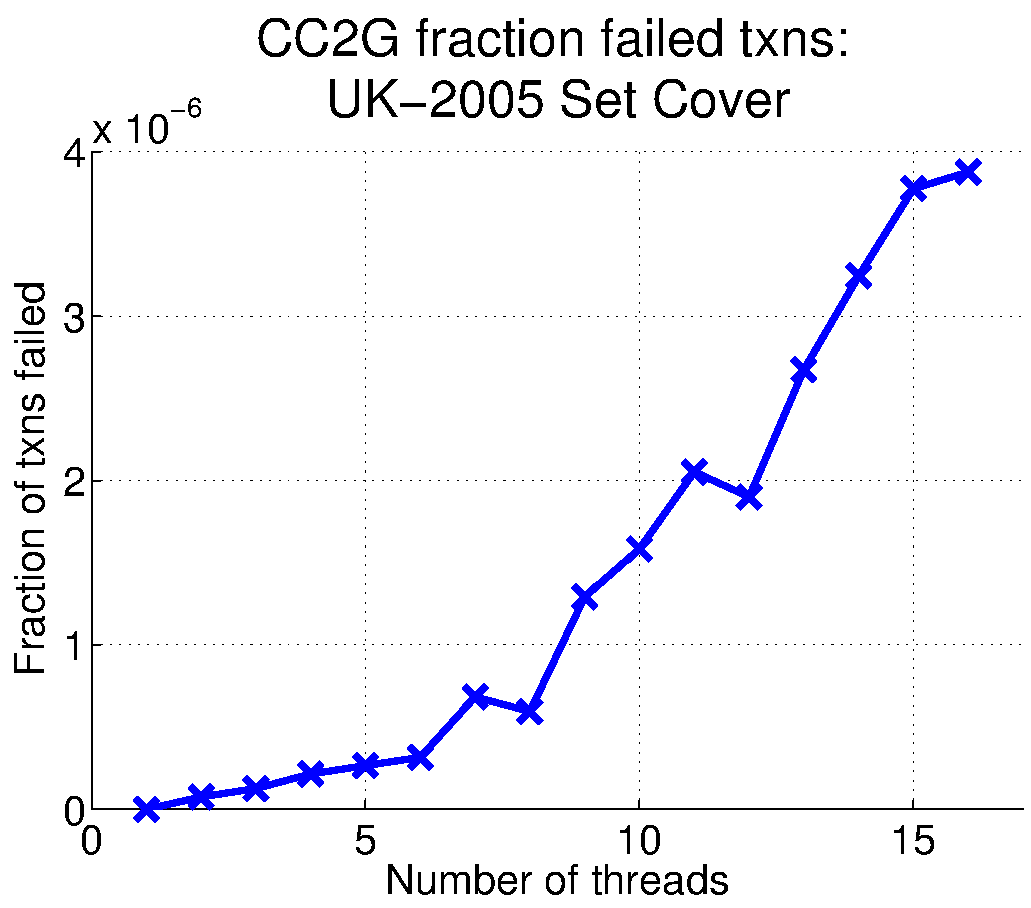
\includegraphics[width=110pt]{images/validated_CC2G_uk2005_setcover.pdf}
			\caption{}
			\label{appfig:validated_CC2G_uk2005_setcover}
	  \end{subfigure} &
	  \begin{subfigure}[b]{0.22\textwidth}
	  	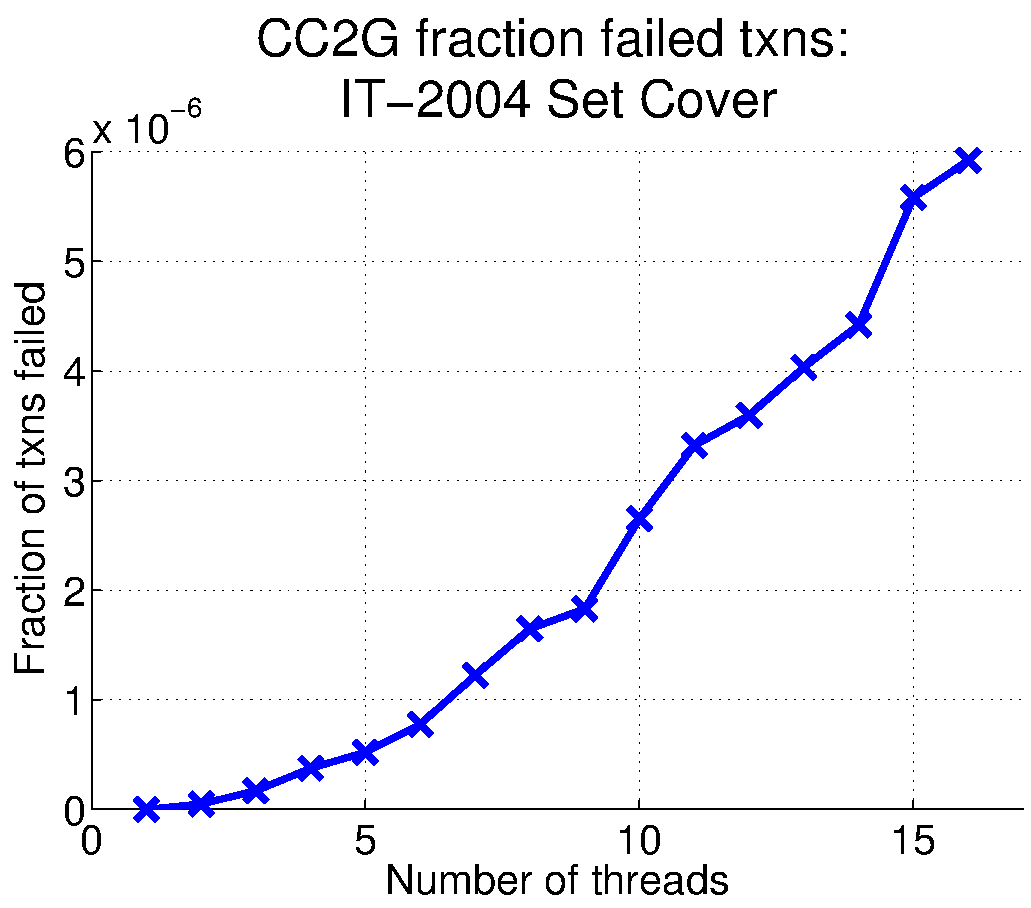
\includegraphics[width=110pt]{images/validated_CC2G_it2004_setcover.pdf}
			\caption{}
			\label{appfig:validated_CC2G_it2004_setcover}
	  \end{subfigure} \\
  \end{tabular}
  \caption{Set cover on 4 real graphs.}
\end{figure}



~\newpage\begin{figure}[ht]
  \centering
  \begin{tabular}{cccc}
	  \begin{subfigure}[b]{0.22\textwidth}
	  	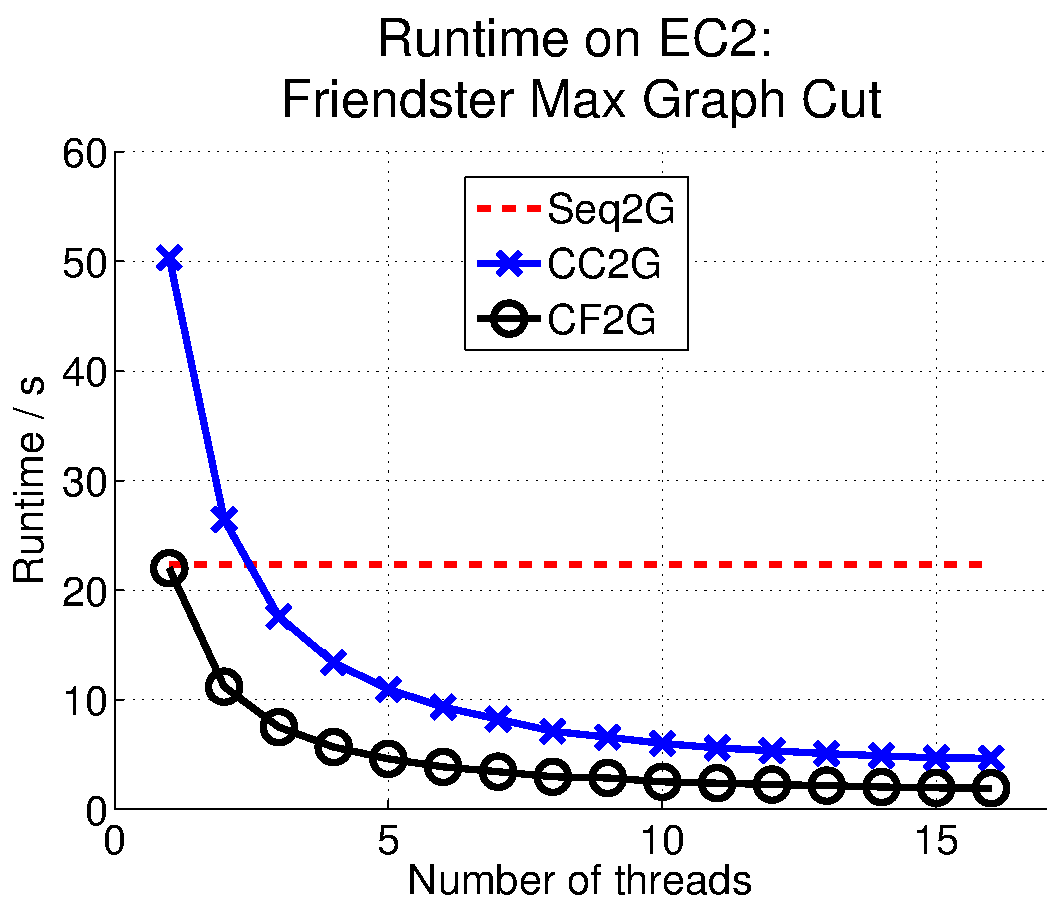
\includegraphics[width=110pt]{images/runtime_friendster10M_maxgraphcut.pdf}
			\caption{}
			\label{appfig:runtime_friendster10M_maxgraphcut}
	  \end{subfigure} &
	  \begin{subfigure}[b]{0.22\textwidth}
	  	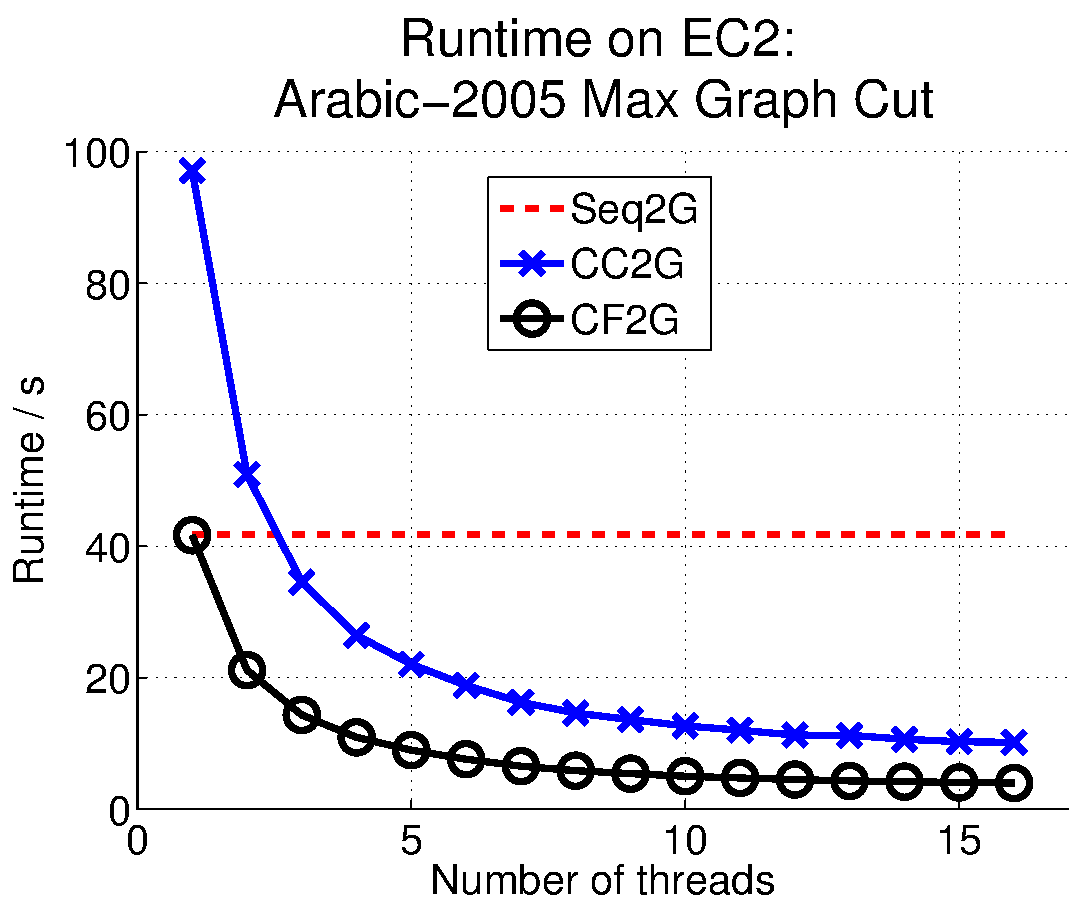
\includegraphics[width=110pt]{images/runtime_arabic2005_maxgraphcut.pdf}
			\caption{}
			\label{appfig:runtime_arabic2005_maxgraphcut}
	  \end{subfigure} &
	  \begin{subfigure}[b]{0.22\textwidth}
	  	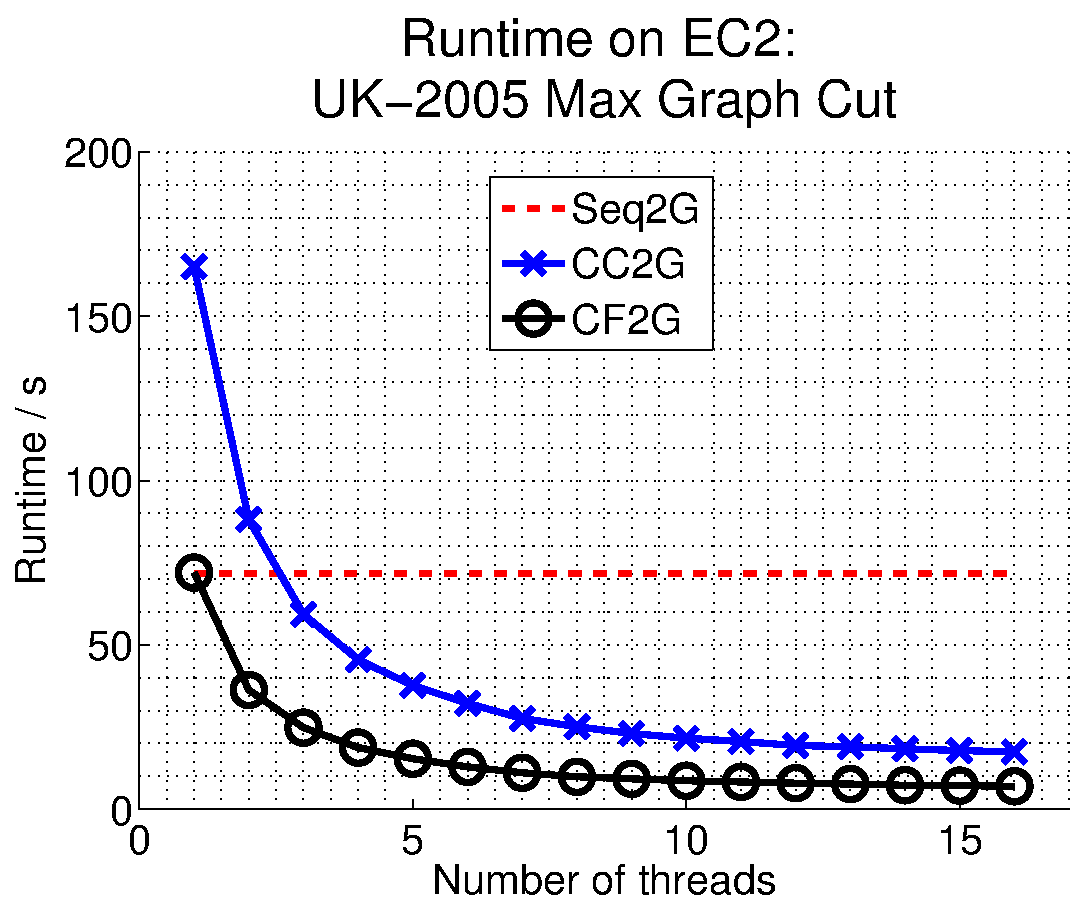
\includegraphics[width=110pt]{images/runtime_uk2005_maxgraphcut.pdf}
			\caption{}
			\label{appfig:runtime_uk2005_maxgraphcut}
	  \end{subfigure} &
	  \begin{subfigure}[b]{0.22\textwidth}
	  	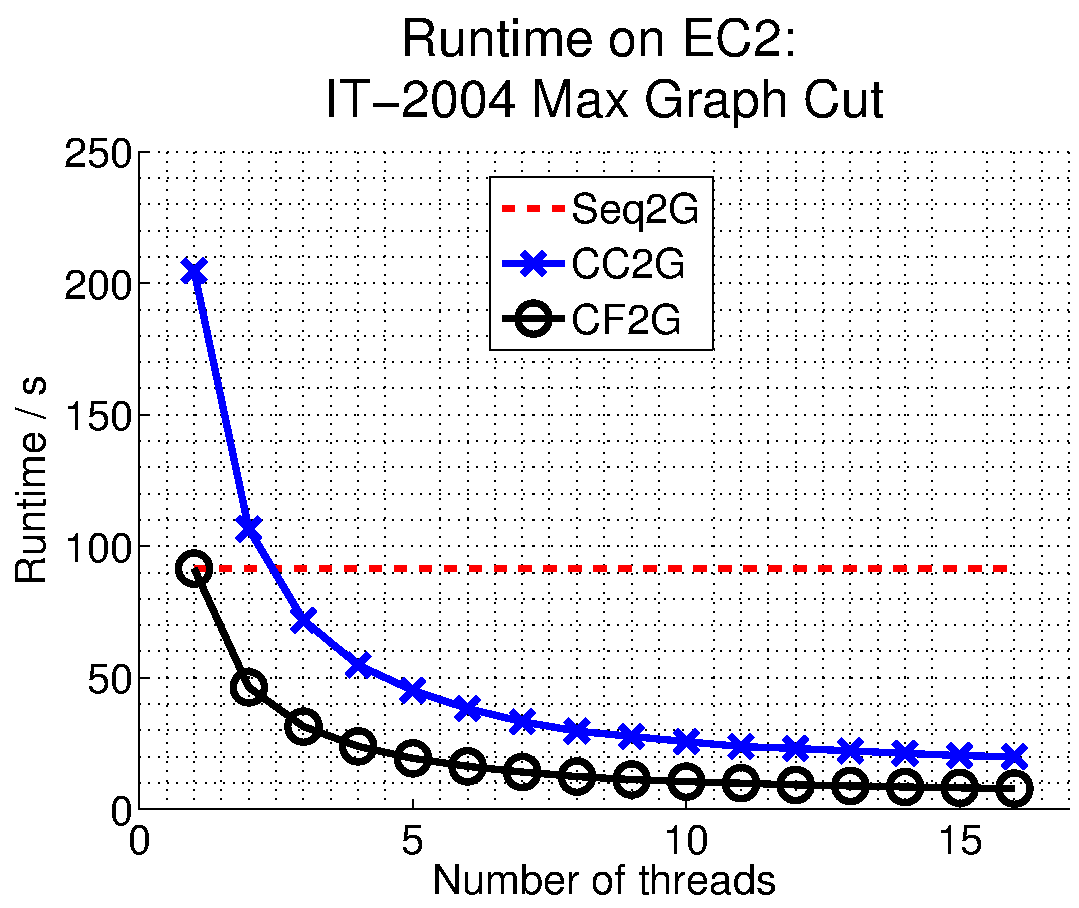
\includegraphics[width=110pt]{images/runtime_it2004_maxgraphcut.pdf}
			\caption{}
			\label{appfig:runtime_it2004_maxgraphcut}
	  \end{subfigure} \\
	  \begin{subfigure}[b]{0.22\textwidth}
	  	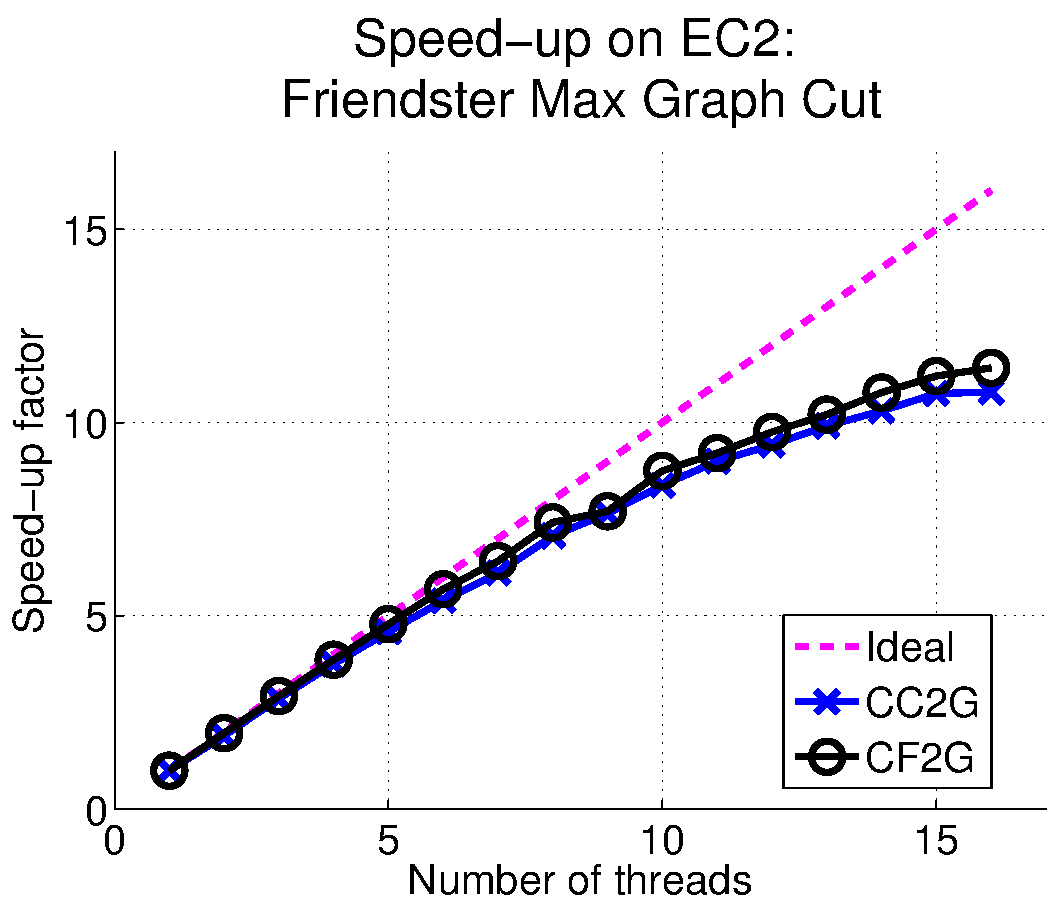
\includegraphics[width=110pt]{images/speedup_friendster10M_maxgraphcut.pdf}
			\caption{}
			\label{appfig:speedup_friendster10M_maxgraphcut}
	  \end{subfigure} &
	  \begin{subfigure}[b]{0.22\textwidth}
	  	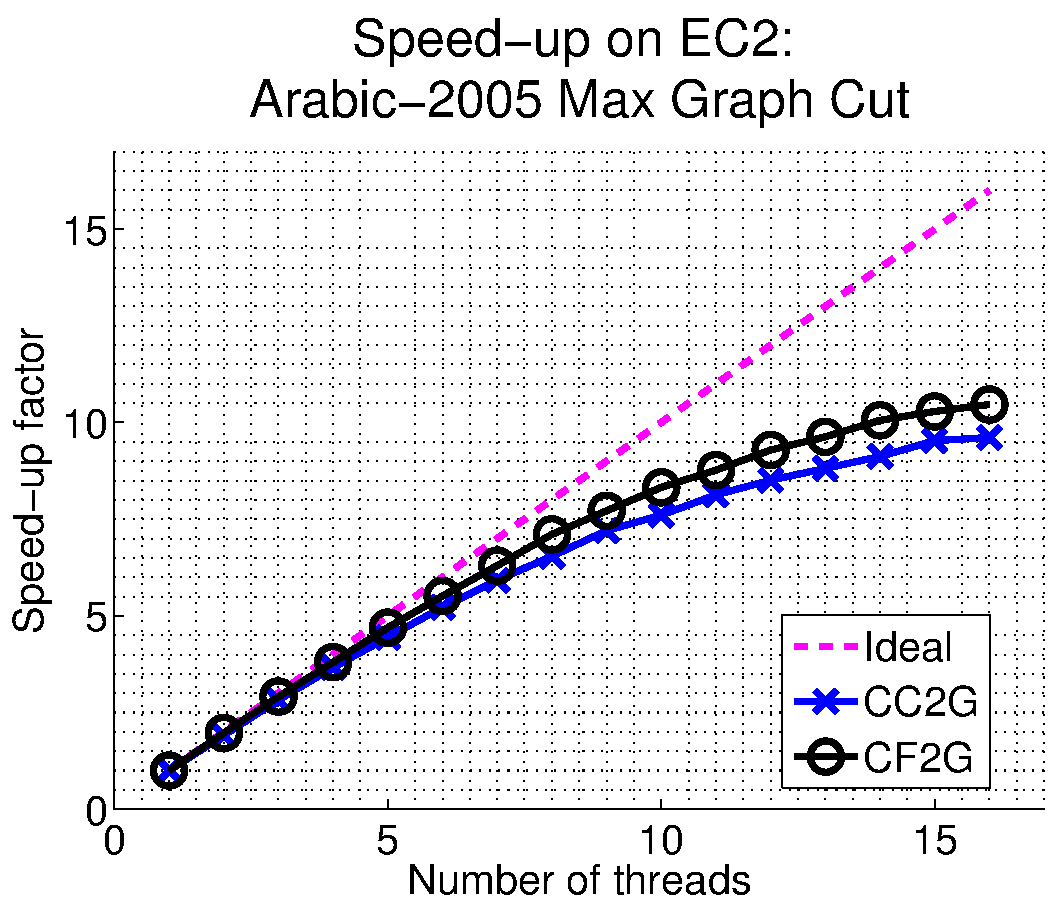
\includegraphics[width=110pt]{images/speedup_arabic2005_maxgraphcut.pdf}
			\caption{}
			\label{appfig:speedup_arabic2005_maxgraphcut}
	  \end{subfigure} &
	  \begin{subfigure}[b]{0.22\textwidth}
	  	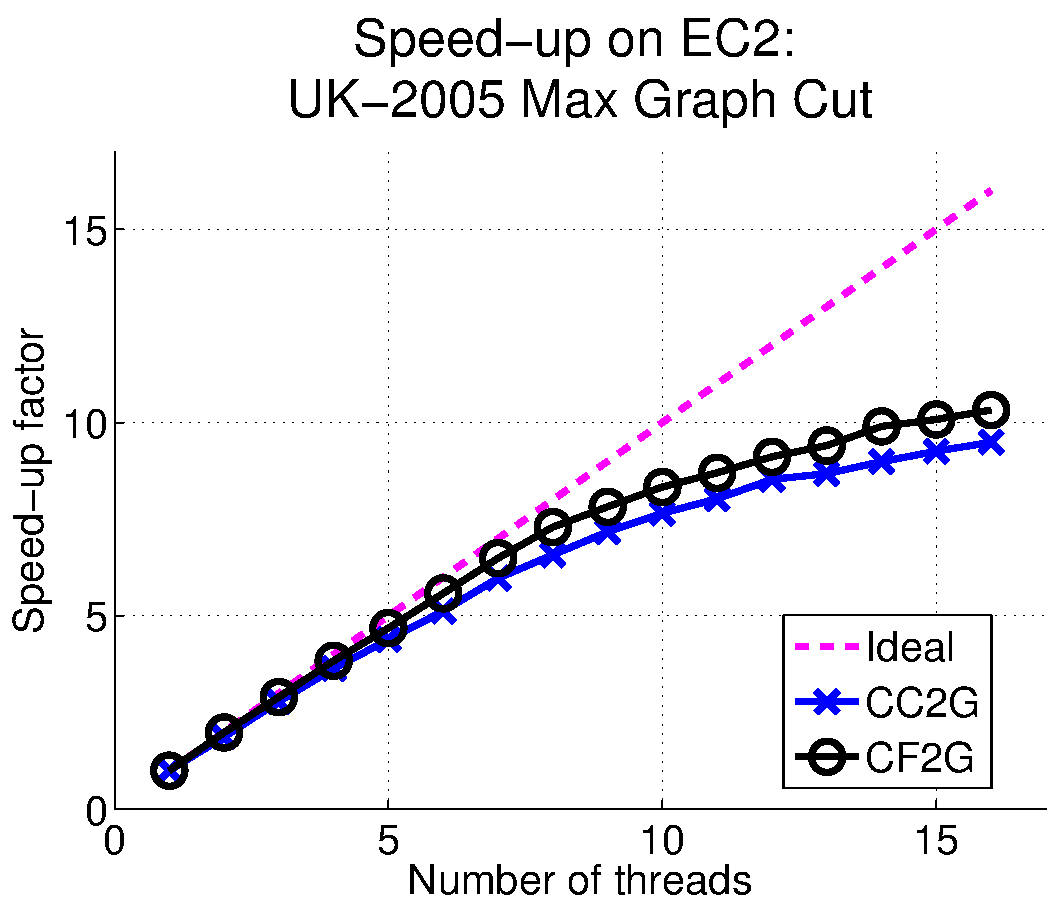
\includegraphics[width=110pt]{images/speedup_uk2005_maxgraphcut.pdf}
			\caption{}
			\label{appfig:speedup_uk2005_maxgraphcut}
	  \end{subfigure} &
	  \begin{subfigure}[b]{0.22\textwidth}
	  	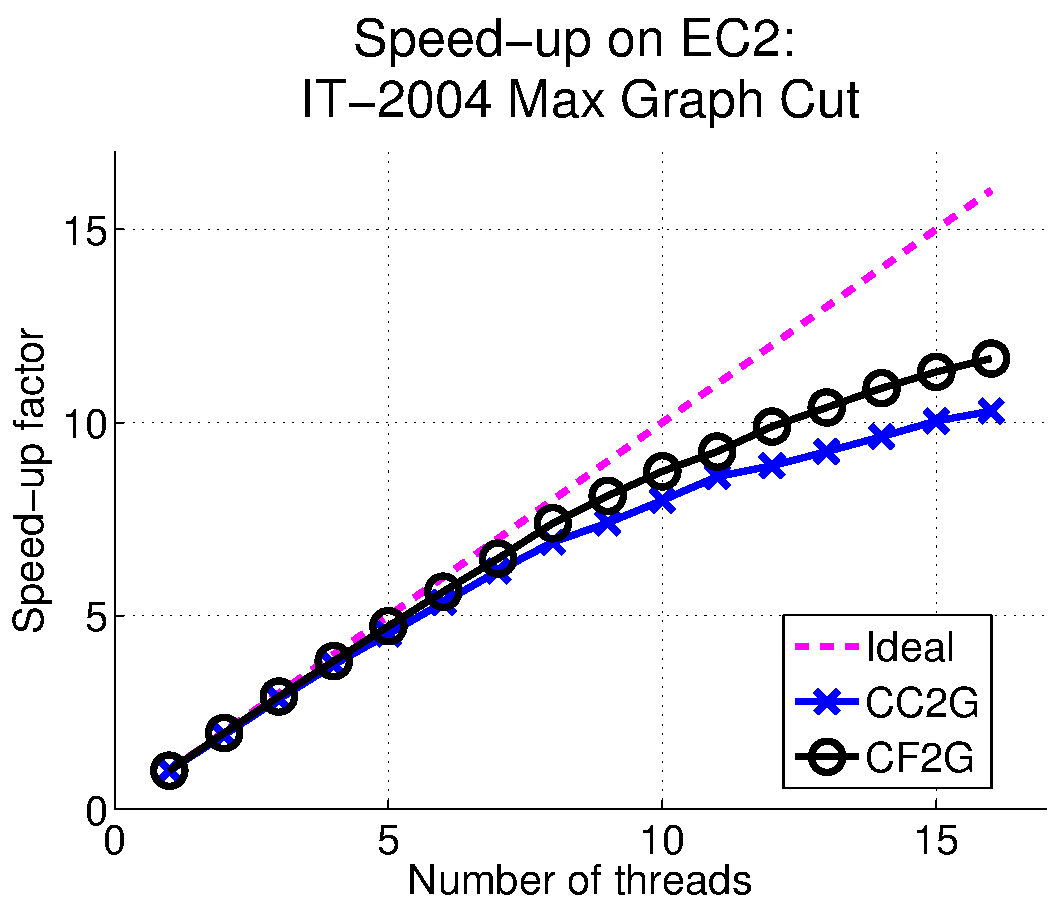
\includegraphics[width=110pt]{images/speedup_it2004_maxgraphcut.pdf}
			\caption{}
			\label{appfig:speedup_it2004_maxgraphcut}
	  \end{subfigure} \\
	  \begin{subfigure}[b]{0.22\textwidth}
	  	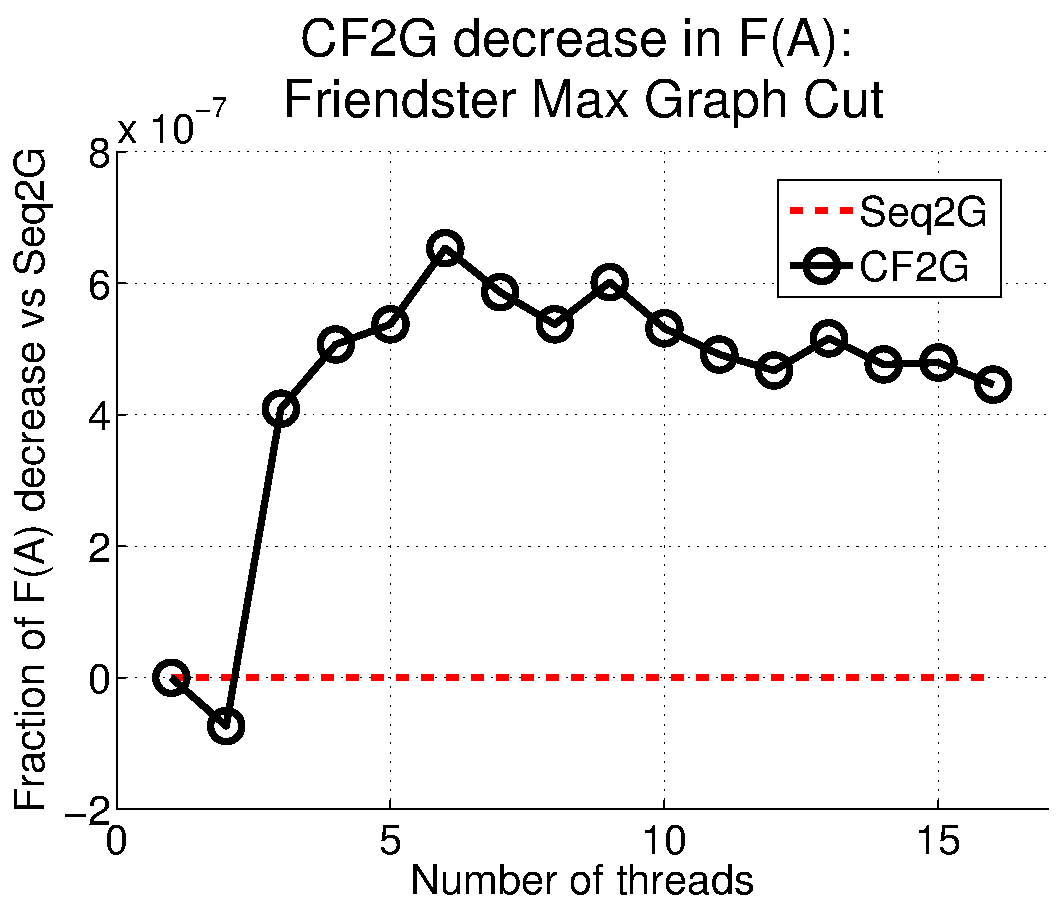
\includegraphics[width=110pt]{images/diffFA_CF2G_friendster10M_maxgraphcut.pdf}
			\caption{}
			\label{appfig:diffFA_CF2G_friendster10M_maxgraphcut}
	  \end{subfigure} &
	  \begin{subfigure}[b]{0.22\textwidth}
	  	\includegraphics[width=110pt]{images/diffFA_CF2G_arabic2005_maxgraphcut.pdf}
			\caption{}
			\label{appfig:diffFA_CF2G_arabic2005_maxgraphcut}
	  \end{subfigure} &
	  \begin{subfigure}[b]{0.22\textwidth}
	  	\includegraphics[width=110pt]{images/diffFA_CF2G_uk2005_maxgraphcut.pdf}
			\caption{}
			\label{appfig:diffFA_CF2G_uk2005_maxgraphcut}
	  \end{subfigure} &
	  \begin{subfigure}[b]{0.22\textwidth}
	  	\includegraphics[width=110pt]{images/diffFA_CF2G_it2004_maxgraphcut.pdf}
			\caption{}
			\label{appfig:diffFA_CF2G_it2004_maxgraphcut}
	  \end{subfigure} \\
	  \begin{subfigure}[b]{0.22\textwidth}
	  	\includegraphics[width=110pt]{images/validated_CC2G_friendster10M_maxgraphcut.pdf}
			\caption{}
			\label{appfig:validated_CC2G_friendster10M_maxgraphcut}
	  \end{subfigure} &
	  \begin{subfigure}[b]{0.22\textwidth}
	  	\includegraphics[width=110pt]{images/validated_CC2G_arabic2005_maxgraphcut.pdf}
			\caption{}
			\label{appfig:validated_CC2G_arabic2005_maxgraphcut}
	  \end{subfigure} &
	  \begin{subfigure}[b]{0.22\textwidth}
	  	\includegraphics[width=110pt]{images/validated_CC2G_uk2005_maxgraphcut.pdf}
			\caption{}
			\label{appfig:validated_CC2G_uk2005_maxgraphcut}
	  \end{subfigure} &
	  \begin{subfigure}[b]{0.22\textwidth}
	  	\includegraphics[width=110pt]{images/validated_CC2G_it2004_maxgraphcut.pdf}
			\caption{}
			\label{appfig:validated_CC2G_it2004_maxgraphcut}
	  \end{subfigure} \\
  \end{tabular}
  \caption{Max graph cut on 4 real graphs.}
\end{figure}





~\newpage\begin{figure}[ht]
  \centering
  \begin{tabular}{cccc}
	  \begin{subfigure}[h]{0.22\textwidth}
	  	\includegraphics[width=110pt]{images/runtime_ring_setcover.pdf}
			\caption{}
			\label{appfig:runtime_ring_setcover}
	  \end{subfigure} &
	  \begin{subfigure}[h]{0.22\textwidth}
	  	\includegraphics[width=110pt]{images/speedup_ring_setcover.pdf}
			\caption{}
			\label{appfig:speedup_ring_setcover}
	  \end{subfigure} &
	  \begin{subfigure}[h]{0.22\textwidth}
	  	\includegraphics[width=110pt]{images/diffFA_CF2G_ring_setcover.pdf}
			\caption{}
			\label{appfig:diffFA_CF2G_ring_setcover}
	  \end{subfigure} &
	  \begin{subfigure}[h]{0.22\textwidth}
	  	\includegraphics[width=110pt]{images/validated_CC2G_ring_setcover.pdf}
			\caption{}
			\label{appfig:validated_CC2G_ring_setcover}
	  \end{subfigure} \\
	  \begin{subfigure}[h]{0.22\textwidth}
	  	\includegraphics[width=110pt]{images/runtime_ring_maxgraphcut.pdf}
			\caption{}
			\label{appfig:runtime_ring_maxgraphcut}
	  \end{subfigure} &
	  \begin{subfigure}[h]{0.22\textwidth}
	  	\includegraphics[width=110pt]{images/speedup_ring_maxgraphcut.pdf}
			\caption{}
			\label{appfig:speedup_ring_maxgraphcut}
	  \end{subfigure} &
	  \begin{subfigure}[h]{0.22\textwidth}
	  	\includegraphics[width=110pt]{images/diffFA_CF2G_ring_maxgraphcut.pdf}
			\caption{}
			\label{appfig:diffFA_CF2G_ring_maxgraphcut}
	  \end{subfigure} &
	  \begin{subfigure}[h]{0.22\textwidth}
	  	\includegraphics[width=110pt]{images/validated_CC2G_ring_maxgraphcut.pdf}
			\caption{}
			\label{appfig:validated_CC2G_ring_maxgraphcut.pdf}
	  \end{subfigure} \\
  \end{tabular}
  \caption{\footnotesize Experimental results for ring graph on set cover problem.}
\label{appfig:results_adversarial}
\end{figure}











~\newpage\section{Full experiment results,  partitioning with work stealing}
\label{app:exptresults_partition}
\begin{figure}[ht]
  \centering
  \begin{tabular}{cccc}
	  \begin{subfigure}[b]{0.22\textwidth}
	  	\includegraphics[width=110pt]{images_partition/runtime_erdosrenyi_maxgraphcut.pdf}
			\caption{}
			\label{appfig:partition:runtime_erdosrenyi_maxgraphcut}
	  \end{subfigure} &
	  \begin{subfigure}[b]{0.22\textwidth}
	  	\includegraphics[width=110pt]{images_partition/runtime_erdosrenyi_setcover.pdf}
			\caption{}
			\label{appfig:partition:runtime_erdosrenyi_setcover}
	  \end{subfigure} &
	  \begin{subfigure}[b]{0.22\textwidth}
	  	\includegraphics[width=110pt]{images_partition/runtime_zigzag_maxgraphcut.pdf}
			\caption{}
			\label{appfig:partition:runtime_zigzag_maxgraphcut}
	  \end{subfigure} &
	  \begin{subfigure}[b]{0.22\textwidth}
	  	\includegraphics[width=110pt]{images_partition/runtime_zigzag_setcover.pdf}
			\caption{}
			\label{appfig:partition:runtime_zigzag_setcover}
	  \end{subfigure} \\
	  \begin{subfigure}[b]{0.22\textwidth}
	  	\includegraphics[width=110pt]{images_partition/speedup_erdosrenyi_maxgraphcut.pdf}
			\caption{}
			\label{appfig:partition:speedup_erdosrenyi_maxgraphcut}
	  \end{subfigure} &
	  \begin{subfigure}[b]{0.22\textwidth}
	  	\includegraphics[width=110pt]{images_partition/speedup_erdosrenyi_setcover.pdf}
			\caption{}
			\label{appfig:partition:speedup_erdosrenyi_setcover}
	  \end{subfigure} &
	  \begin{subfigure}[b]{0.22\textwidth}
	  	\includegraphics[width=110pt]{images_partition/speedup_zigzag_maxgraphcut.pdf}
			\caption{}
			\label{appfig:partition:speedup_zigzag_maxgraphcut}
	  \end{subfigure} &
	  \begin{subfigure}[b]{0.22\textwidth}
	  	\includegraphics[width=110pt]{images_partition/speedup_zigzag_setcover.pdf}
			\caption{}
			\label{appfig:partition:speedup_zigzag_setcover}
	  \end{subfigure} \\
	  \begin{subfigure}[b]{0.22\textwidth}
	  	\includegraphics[width=110pt]{images_partition/diffFA_CF2G_erdosrenyi_maxgraphcut.pdf}
			\caption{}
			\label{appfig:partition:diffFA_CF2G_erdosrenyi_maxgraphcut}
	  \end{subfigure} &
	  \begin{subfigure}[b]{0.22\textwidth}
	  	\includegraphics[width=110pt]{images_partition/diffFA_CF2G_erdosrenyi_setcover.pdf}
			\caption{}
			\label{appfig:partition:diffFA_CF2G_erdosrenyi_setcover}
	  \end{subfigure} &
	  \begin{subfigure}[b]{0.22\textwidth}
	  	\includegraphics[width=110pt]{images_partition/diffFA_CF2G_zigzag_maxgraphcut.pdf}
			\caption{}
			\label{appfig:partition:diffFA_CF2G_zigzag_maxgraphcut}
	  \end{subfigure} &
	  \begin{subfigure}[b]{0.22\textwidth}
	  	\includegraphics[width=110pt]{images_partition/diffFA_CF2G_zigzag_setcover.pdf}
			\caption{}
			\label{appfig:partition:diffFA_CF2G_zigzag_setcover}
	  \end{subfigure} \\
	  \begin{subfigure}[b]{0.22\textwidth}
	  	\includegraphics[width=110pt]{images_partition/validated_CC2G_erdosrenyi_maxgraphcut.pdf}
			\caption{}
			\label{appfig:partition:validated_CC2G_erdosrenyi_maxgraphcut}
	  \end{subfigure} &
	  \begin{subfigure}[b]{0.22\textwidth}
	  	\includegraphics[width=110pt]{images_partition/validated_CC2G_erdosrenyi_setcover.pdf}
			\caption{}
			\label{appfig:partition:validated_CC2G_erdosrenyi_setcover}
	  \end{subfigure} &
	  \begin{subfigure}[b]{0.22\textwidth}
	  	\includegraphics[width=110pt]{images_partition/validated_CC2G_zigzag_maxgraphcut.pdf}
			\caption{}
			\label{appfig:partition:validated_CC2G_zigzag_maxgraphcut}
	  \end{subfigure} &
	  \begin{subfigure}[b]{0.22\textwidth}
	  	\includegraphics[width=110pt]{images_partition/validated_CC2G_zigzag_setcover.pdf}
			\caption{}
			\label{appfig:partition:validated_CC2G_zigzag_setcover}
	  \end{subfigure} \\
  \end{tabular}
  \caption{Experimental results (with partitioning) on Erdos-Renyi and ZigZag synthetic graphs.}
\end{figure}


~\newpage\begin{figure}[ht]
  \centering
  \begin{tabular}{cccc}
	  \begin{subfigure}[b]{0.22\textwidth}
	  	\includegraphics[width=110pt]{images_partition/runtime_friendster_setcover.pdf}
			\caption{}
			\label{appfig:partition:runtime_friendster_setcover}
	  \end{subfigure} &
	  \begin{subfigure}[b]{0.22\textwidth}
	  	\includegraphics[width=110pt]{images_partition/runtime_arabic2005_setcover.pdf}
			\caption{}
			\label{appfig:partition:runtime_arabic2005_setcover}
	  \end{subfigure} &
	  \begin{subfigure}[b]{0.22\textwidth}
	  	\includegraphics[width=110pt]{images_partition/runtime_uk2005_setcover.pdf}
			\caption{}
			\label{appfig:partition:runtime_uk2005_setcover}
	  \end{subfigure} &
	  \begin{subfigure}[b]{0.22\textwidth}
	  	\includegraphics[width=110pt]{images_partition/runtime_it2004_setcover.pdf}
			\caption{}
			\label{appfig:partition:runtime_it2004_setcover}
	  \end{subfigure} \\
	  \begin{subfigure}[b]{0.22\textwidth}
	  	\includegraphics[width=110pt]{images_partition/speedup_friendster_setcover.pdf}
			\caption{}
			\label{appfig:partition:speedup_friendster_setcover}
	  \end{subfigure} &
	  \begin{subfigure}[b]{0.22\textwidth}
	  	\includegraphics[width=110pt]{images_partition/speedup_arabic2005_setcover.pdf}
			\caption{}
			\label{appfig:partition:speedup_arabic2005_setcover}
	  \end{subfigure} &
	  \begin{subfigure}[b]{0.22\textwidth}
	  	\includegraphics[width=110pt]{images_partition/speedup_uk2005_setcover.pdf}
			\caption{}
			\label{appfig:partition:speedup_uk2005_setcover}
	  \end{subfigure} &
	  \begin{subfigure}[b]{0.22\textwidth}
	  	\includegraphics[width=110pt]{images_partition/speedup_it2004_setcover.pdf}
			\caption{}
			\label{appfig:partition:speedup_it2004_setcover}
	  \end{subfigure} \\
	  \begin{subfigure}[b]{0.22\textwidth}
	  	\includegraphics[width=110pt]{images_partition/diffFA_CF2G_friendster_setcover.pdf}
			\caption{}
			\label{appfig:partition:diffFA_CF2G_friendster_setcover}
	  \end{subfigure} &
	  \begin{subfigure}[b]{0.22\textwidth}
	  	\includegraphics[width=110pt]{images_partition/diffFA_CF2G_arabic2005_setcover.pdf}
			\caption{}
			\label{appfig:partition:diffFA_CF2G_arabic2005_setcover}
	  \end{subfigure} &
	  \begin{subfigure}[b]{0.22\textwidth}
	  	\includegraphics[width=110pt]{images_partition/diffFA_CF2G_uk2005_setcover.pdf}
			\caption{}
			\label{appfig:partition:diffFA_CF2G_uk2005_setcover}
	  \end{subfigure} &
	  \begin{subfigure}[b]{0.22\textwidth}
	  	\includegraphics[width=110pt]{images_partition/diffFA_CF2G_it2004_setcover.pdf}
			\caption{}
			\label{appfig:partition:diffFA_CF2G_it2004_setcover}
	  \end{subfigure} \\
	  \begin{subfigure}[b]{0.22\textwidth}
	  	\includegraphics[width=110pt]{images_partition/validated_CC2G_friendster_setcover.pdf}
			\caption{}
			\label{appfig:partition:validated_CC2G_friendster_setcover}
	  \end{subfigure} &
	  \begin{subfigure}[b]{0.22\textwidth}
	  	\includegraphics[width=110pt]{images_partition/validated_CC2G_arabic2005_setcover.pdf}
			\caption{}
			\label{appfig:partition:validated_CC2G_arabic2005_setcover}
	  \end{subfigure} &
	  \begin{subfigure}[b]{0.22\textwidth}
	  	\includegraphics[width=110pt]{images_partition/validated_CC2G_uk2005_setcover.pdf}
			\caption{}
			\label{appfig:partition:validated_CC2G_uk2005_setcover}
	  \end{subfigure} &
	  \begin{subfigure}[b]{0.22\textwidth}
	  	\includegraphics[width=110pt]{images_partition/validated_CC2G_it2004_setcover.pdf}
			\caption{}
			\label{appfig:partition:validated_CC2G_it2004_setcover}
	  \end{subfigure} \\
  \end{tabular}
  \caption{Set cover (with partitioning) on 4 real graphs.}
\end{figure}



~\newpage\begin{figure}[ht]
  \centering
  \begin{tabular}{cccc}
	  \begin{subfigure}[b]{0.22\textwidth}
	  	\includegraphics[width=110pt]{images_partition/runtime_friendster_maxgraphcut.pdf}
			\caption{}
			\label{appfig:partition:runtime_friendster_maxgraphcut}
	  \end{subfigure} &
	  \begin{subfigure}[b]{0.22\textwidth}
	  	\includegraphics[width=110pt]{images_partition/runtime_arabic2005_maxgraphcut.pdf}
			\caption{}
			\label{appfig:partition:runtime_arabic2005_maxgraphcut}
	  \end{subfigure} &
	  \begin{subfigure}[b]{0.22\textwidth}
	  	\includegraphics[width=110pt]{images_partition/runtime_uk2005_maxgraphcut.pdf}
			\caption{}
			\label{appfig:partition:runtime_uk2005_maxgraphcut}
	  \end{subfigure} &
	  \begin{subfigure}[b]{0.22\textwidth}
	  	\includegraphics[width=110pt]{images_partition/runtime_it2004_maxgraphcut.pdf}
			\caption{}
			\label{appfig:partition:runtime_it2004_maxgraphcut}
	  \end{subfigure} \\
	  \begin{subfigure}[b]{0.22\textwidth}
	  	\includegraphics[width=110pt]{images_partition/speedup_friendster_maxgraphcut.pdf}
			\caption{}
			\label{appfig:partition:speedup_friendster_maxgraphcut}
	  \end{subfigure} &
	  \begin{subfigure}[b]{0.22\textwidth}
	  	\includegraphics[width=110pt]{images_partition/speedup_arabic2005_maxgraphcut.pdf}
			\caption{}
			\label{appfig:partition:speedup_arabic2005_maxgraphcut}
	  \end{subfigure} &
	  \begin{subfigure}[b]{0.22\textwidth}
	  	\includegraphics[width=110pt]{images_partition/speedup_uk2005_maxgraphcut.pdf}
			\caption{}
			\label{appfig:partition:speedup_uk2005_maxgraphcut}
	  \end{subfigure} &
	  \begin{subfigure}[b]{0.22\textwidth}
	  	\includegraphics[width=110pt]{images_partition/speedup_it2004_maxgraphcut.pdf}
			\caption{}
			\label{appfig:partition:speedup_it2004_maxgraphcut}
	  \end{subfigure} \\
	  \begin{subfigure}[b]{0.22\textwidth}
	  	\includegraphics[width=110pt]{images_partition/diffFA_CF2G_friendster_maxgraphcut.pdf}
			\caption{}
			\label{appfig:partition:diffFA_CF2G_friendster_maxgraphcut}
	  \end{subfigure} &
	  \begin{subfigure}[b]{0.22\textwidth}
	  	\includegraphics[width=110pt]{images_partition/diffFA_CF2G_arabic2005_maxgraphcut.pdf}
			\caption{}
			\label{appfig:partition:diffFA_CF2G_arabic2005_maxgraphcut}
	  \end{subfigure} &
	  \begin{subfigure}[b]{0.22\textwidth}
	  	\includegraphics[width=110pt]{images_partition/diffFA_CF2G_uk2005_maxgraphcut.pdf}
			\caption{}
			\label{appfig:partition:diffFA_CF2G_uk2005_maxgraphcut}
	  \end{subfigure} &
	  \begin{subfigure}[b]{0.22\textwidth}
	  	\includegraphics[width=110pt]{images_partition/diffFA_CF2G_it2004_maxgraphcut.pdf}
			\caption{}
			\label{appfig:partition:diffFA_CF2G_it2004_maxgraphcut}
	  \end{subfigure} \\
	  \begin{subfigure}[b]{0.22\textwidth}
	  	\includegraphics[width=110pt]{images_partition/validated_CC2G_friendster_maxgraphcut.pdf}
			\caption{}
			\label{appfig:partition:validated_CC2G_friendster_maxgraphcut}
	  \end{subfigure} &
	  \begin{subfigure}[b]{0.22\textwidth}
	  	\includegraphics[width=110pt]{images_partition/validated_CC2G_arabic2005_maxgraphcut.pdf}
			\caption{}
			\label{appfig:partition:validated_CC2G_arabic2005_maxgraphcut}
	  \end{subfigure} &
	  \begin{subfigure}[b]{0.22\textwidth}
	  	\includegraphics[width=110pt]{images_partition/validated_CC2G_uk2005_maxgraphcut.pdf}
			\caption{}
			\label{appfig:partition:validated_CC2G_uk2005_maxgraphcut}
	  \end{subfigure} &
	  \begin{subfigure}[b]{0.22\textwidth}
	  	\includegraphics[width=110pt]{images_partition/validated_CC2G_it2004_maxgraphcut.pdf}
			\caption{}
			\label{appfig:partition:validated_CC2G_it2004_maxgraphcut}
	  \end{subfigure} \\
  \end{tabular}
  \caption{Max graph cut (with partitioning) on 4 real graphs.}
\end{figure}





~\newpage\begin{figure}[ht]
  \centering
  \begin{tabular}{cccc}
	  \begin{subfigure}[h]{0.22\textwidth}
	  	\includegraphics[width=110pt]{images_partition/runtime_ring_setcover.pdf}
			\caption{}
			\label{appfig:partition:runtime_ring_setcover}
	  \end{subfigure} &
	  \begin{subfigure}[h]{0.22\textwidth}
	  	\includegraphics[width=110pt]{images_partition/speedup_ring_setcover.pdf}
			\caption{}
			\label{appfig:partition:speedup_ring_setcover}
	  \end{subfigure} &
	  \begin{subfigure}[h]{0.22\textwidth}
	  	\includegraphics[width=110pt]{images_partition/diffFA_CF2G_ring_setcover.pdf}
			\caption{}
			\label{appfig:partition:diffFA_CF2G_ring_setcover}
	  \end{subfigure} &
	  \begin{subfigure}[h]{0.22\textwidth}
	  	\includegraphics[width=110pt]{images_partition/validated_CC2G_ring_setcover.pdf}
			\caption{}
			\label{appfig:partition:validated_CC2G_ring_setcover}
	  \end{subfigure} \\
	  \begin{subfigure}[h]{0.22\textwidth}
	  	\includegraphics[width=110pt]{images_partition/runtime_ring_maxgraphcut.pdf}
			\caption{}
			\label{appfig:partition:runtime_ring_maxgraphcut}
	  \end{subfigure} &
	  \begin{subfigure}[h]{0.22\textwidth}
	  	\includegraphics[width=110pt]{images_partition/speedup_ring_maxgraphcut.pdf}
			\caption{}
			\label{appfig:partition:speedup_ring_maxgraphcut}
	  \end{subfigure} &
	  \begin{subfigure}[h]{0.22\textwidth}
	  	\includegraphics[width=110pt]{images_partition/diffFA_CF2G_ring_maxgraphcut.pdf}
			\caption{}
			\label{appfig:partition:diffFA_CF2G_ring_maxgraphcut}
	  \end{subfigure} &
	  \begin{subfigure}[h]{0.22\textwidth}
	  	\includegraphics[width=110pt]{images_partition/validated_CC2G_ring_maxgraphcut.pdf}
			\caption{}
			\label{appfig:partition:validated_CC2G_ring_maxgraphcut.pdf}
	  \end{subfigure} \\
  \end{tabular}
  \caption{\footnotesize Experimental results (with partitioning) for ring graph on set cover problem.}
\label{appfig:partition:results_adversarial}
\end{figure}

~




%%%%%%%%%%%%%%%%%%%%%%%%%%%%%%%%%%%%%%%%%%%%%%%%%%%%%%%%%%%%%%%%%%%%%%%%%%%%%%%%%%%%%%%%%%%%%%%%%%%%%%%%%%%%%%%%
\begin{comment}
\section{Discussion on $\rho_i$}

\section{\hogwild{} approximation for monotone $F$}
\subsection{Proof for monotone functions}
\begin{lem}\label{lem:singleelement_monotone} If $F$ is monotone submodular, for every $1 \leq i \leq n$,
\[E[F(O^{i-1})-F(O^i)] \leq \frac{1}{2(1-\kappa_F)} E[f(A^i) - f(A^{i-1}) + f(B^i) - f(B^{i-1})].\]
\end{lem}
\begin{proof}
Since $F$ is monotone, we only have to check the case where $0 \leq \Delta_+(i) \leq \Delta_+^{\max}(i)$ and $0 \leq \Delta_-(i) \leq \Delta_-^{\max}(i)$.
Following the proof structure of Case 8 in Lemma \ref{lem:singleelement}, we get
\begin{align*}
E[f(A^i) - f(A^{i-1}) | A^{i-1}, j] &\geq \frac{(1+\kappa_F)\Delta_+^{\max}(i)^2}{\Delta_+^{\max}(i) + \Delta_-^{\max}(i)}\\
E[f(B^i) - f(B^{i-1}) | A^{i-1}, j] &\geq \frac{(1+\kappa_F)\Delta_-^{\max}(i)^2}{\Delta_+^{\max}(i) + \Delta_-^{\max}(i)}\\
E(f(O^{i-1}) - f(O^i) | A^{i-1}, j] &\leq \frac{\Delta_+^{\max}(i)\Delta_-^{\max}(i)}{\Delta_+^{\max}(i) + \Delta_-^{\max}(i)}
\end{align*}
\begin{align*}
&E[F(O^{i-1}) - F(O^i) | A^{i-1}, j] - \frac{1}{2(1-\kappa_F)} E[f(A^i) - f(A^{i-1}) + f(B^i) - f(B^{i-1})| A^{i-1}, j]\\
&\leq \frac{1/2}{\Delta_+^{\max}(i) + \Delta_-^{\max}(i)}\bigg[
2\Delta_+^{\max}(i)\Delta_-^{\max}(i)
- \Delta_-^{\max}(i)^2
- \Delta_+^{\max}(i)^2
\bigg]\\
&= \frac{1/2}{\Delta_+^{\max}(i) + \Delta_-^{\max}(i)}\bigg[-(\Delta_+^{\max}(i) - \Delta_-^{\max}(i))^2\bigg]\\
&\leq 0.
\end{align*}
\end{proof}

\begin{thm}\label{thm:randomapprox_monotone} Let $F$ be a non-negative monotone submodular function.
The \hogwild{} bidirectional greedy algorithm solves the unconstrained problem $\max_{A\subset V} F(A)$ with approximation
\[
E[F(A)] \geq \frac{1-\kappa_F}{2-\kappa_F}F^*,
\]
where $A$ is the algorithm output, $F^*$ is the optimal value, and $\kappa_F$ is the total curvature of the function.
\end{thm}
\begin{proof}
Summing up the statement of Lemma \ref{lem:singleelement_monotone} for all $i$ gives us a telescoping sum, which reduces to:
\begin{align*}
E[F(O^0)-F(O^n)]
&\leq \frac{1}{2(1-\kappa_F)} E[F(A^n) - F(A^0) + F(B^n) - F(B^0)]\\
&\leq \frac{1}{2(1-\kappa_F)} E[F(A^n) + F(B^n)].
\end{align*}
Note that $O^0 = OPT$ and $O^n = A^n = B^n$, so $E[F(A^n)] \geq \frac{1-\kappa_F}{2-\kappa} F(OPT)$.
\end{proof}
\end{comment}
%%%%%%%%%%%%%%%%%%%%%%%%%%%%%%%%%%%%%%%%%%%%%%%%%%%%%%%%%%%%%%%%%%%%%%%%%%%%%%%%%%%%%%%%%%%%%%%%%%%%%%%%%%%%%%%%

\end{document}


% This document was modified from the file originally made available by
% Pat Langley and Andrea Danyluk for ICML-2K. This version was
% created by Lise Getoor and Tobias Scheffer, it was slightly modified
% from the 2010 version by Thorsten Joachims & Johannes Fuernkranz,
% slightly modified from the 2009 version by Kiri Wagstaff and
% Sam Roweis's 2008 version, which is slightly modified from
% Prasad Tadepalli's 2007 version which is a lightly
% changed version of the previous year's version by Andrew Moore,
% which was in turn edited from those of Kristian Kersting and
% Codrina Lauth. Alex Smola contributed to the algorithmic style files.
